%
\documentclass[hdr, twoside, final, memoir]{unswthesis}
\usepackage{mystyle, graphicx, pdfpages} % all include packages and 
\usepackage{booktabs}
\usepackage{tabularx}
\usepackage[table]{xcolor}
\usepackage{epigraph}
\usepackage{hyperref}
\usepackage{float}
\usepackage{tcolorbox}




\makeatletter
\fancypagestyle{noHeading}{
        \fancyhead{}
        \renewcommand{\headrulewidth}{0pt}
}
\raggedbottom

\thesistitle{Beyond Creative Automation: 
Enabling Human-AI Co-Creativity Through Dialogic Interaction Design}
\thesisschool{School of Computer Science and Engineering}
\thesisauthor{Rodolfo Ocampo}
\thesisZid{z1234567}
\thesisdegree{Doctor of Philosophy}
\thesisdate{June 2025}
\thesissupervisor{Firstname Lastname}% for undergrad theses only
 % Thesis details e.g. Title


\newcommand*\mean[1]{\overline{#1}}
\newcommand*{\Perm}[2]{{}^{#1}\!P_{#2}}

\DeclareGraphicsExtensions{.pdf,.jpeg,.png}
\graphicspath{{2-intro/}{3-literature/}{4-techchapter/}{5-techchapter/}{6-techchapter/}{8-appendices/}}


\newcommand\blankpage{
        \null
        \thispagestyle{empty}
        \addtocounter{page}{-1}
        \newpage
}

% Custom maketitle to exclude dissertation sheet
\renewcommand{\maketitle}%
    {\begin{titlepage}%
        \vspace*{-20mm}%
        \enlargethispage{\footskip}% no footer on cover
	\begin{center}%
          \coverpagefont
          {\largeboldcoverpagefont \ThesisTitle \par}%
          \vskip 0pt plus 8fill
          {\largecoverpagefont \ThesisAuthor \par}%
          \vskip 0pt plus 8fill
          { A thesis in fulfilment of the requirements for the degree of \\[2ex]
              \ThesisDegreeName \par}%
          \vskip 0pt plus 8fill
          
\includegraphics{unswlogo}
	  \vskip 0pt plus 4fill
          \ThesisSchoolName\par
          \ThesisFacultyName\par
          The University of New South Wales\par
	  \vskip 0pt plus 4fill
          \ThesisDate \par%
	\end{center}\par
    \end{titlepage}
    \clearemptydoublepage
    %\ThesisDissertationSheet  % Commented out to remove dissertation sheet
    %\ThesisOriginalityDeclaration  % Commented out to remove originality declaration
    %\CopyrightAndAuthenticity  % Commented out to remove copyright and authenticity statements
    \setcounter{footnote}{0}
    \let\maketitle\relax}

\begin{document}
    
    \renewcommand{\bibname}{References}
    %% pages in the ``frontmatter'' section have roman numeral page number
    \frontmatter  
    \maketitle
    
    %the forms from GRIS printed as pdf
    %\includepdf[pages=1]{1-pre/GRIS.pdf}
    %\includepdf[pages=1]{1-pre/GRIS2.pdf}
    % \afterpage{\blankpage}

    \chapter{Abstract}

Recent progress in generative artificial intelligence (AI) opens the possibility of human-machine co-creativity. However, realising this possibility depends on answering a key question at the interaction layer. How can we design interactions between humans and AI so that their unique forms of creativity are mutually enhanced and blended, while human agency is maintained? Addressing this question is the core aim of my thesis. 

Numerous interaction design principles exist in the field of human-computer interaction, yet no such principles exist for human-AI co-creativity. This thesis combines an analysis of emerging literature with original interaction design and creative practice-led research to fill this gap. 

Co-creativity requires mutual influence and understanding. However, current linear and request-based human-computer interaction design paradigms are limited in affording such influence and understanding. I argue that modelling dialogue is a promising approach. Consequently, I develop a theoretical framework for dialogic co-creativity where human and computer iteratively interact \textit{through} and \textit{about} the creation. I then use this framework as a navigational lens across three main pieces of research.

First, in Chapter 4, I develop a dialogic co-creative writing system supporting human-AI interaction \textit{through} and \textit{about} the writing process by integrating a collaborative text editor and a conversational space. Across two user studies, I show that this interface leads to greater user involvement and perceived agency, compared to chat-only interfaces.

In Chapter 5, I present a case study conducted in collaboration with a nationally printed Australian magazine, exploring the potential and challenges of image-based generative AI in real-world creative workflows through the co-production of one of their issues. I identify three main challenges: a lack of generative consistency, limited stylistic and structural control, and inadequate support for iterative workflows.

Lastly, in Chapter 6, I describe the creation of two generative public art installations leveraging generative language models for real-time audiovisual performance. Generative AI opens up new creative possibilities in new media practice by assuming novel co-creative roles. However, as described in this Chapter, generative AI systems remain difficult to steer towards human creative intent.

In the final chapter, I argue that the dominant current interaction design paradigms of prompting and purely conversational interfaces lead users to primarily assume roles in the `intentional space’ of goals and ideas, while AI assumes creative execution roles in the `action space’. As a result, users become increasingly detached from the creative process, leading to what I describe as \textit{severed creative agency}: a disconnect between creative intention and action. This stems from two main causes: the difficulty in steering generative AI systems and a reduced level of involvement in the creative process. However, at the same tine, generative AI has the potential to enable new creative operations by collaboratively enhancing human creativity. Balancing this tension between creative augmentation and automation is what I describe as the \textit{core tension in human-AI co-creativity}. 

This thesis contributes to our understanding of how to develop co-creative systems with confidence. I provide a set of 11 actionable design principles for creating more effective co-creative AI systems, derived from the dialogic co-creativity framework and focused on enabling mutual understanding, adaptation, enhanced user involvement and human creative agency.

It is my hope that this thesis similarly inspires artists and practitioners to explore the creative possibilities at the intersection with other intelligences.

    \chapter{Acknowledgements}
    \chapter{Publications and Presentations}

\section*{List of Publications}

\begin{itemize}
    \item \textbf{A Framework for Dialogue-Based Human-AI Creative Collaboration.} Ocampo, Rodolfo, Bown, Oliver, \& Grace, Kazjon. (2022). In \textit{Proceedings of the CHI 2022 Workshop on Generative AI and HCI}. New Orleans, USA. (paper)
    
    \item \textbf{Using GPT-3 to Achieve Semantically Relevant Data Sonification for an Art Installation.} Ocampo, Rodolfo, Bown, Oliver, Wright, Brendan, Shave, Justin, \& Pegram, Caroline. (2023). In \textit{Artificial Intelligence in Music, Sound, Art and Design: 12th International Conference}. Brno, Czech Republic. (paper)
    
    \item \textbf{The Human-Built Environment-Natural Environment Relation—An Immersive Multisensory Exploration with 'System of a Sound'.} Ocampo, Rodolfo, Bown, Oliver, Wright, Brendan, \& Shave, Justin. (2023). In \textit{Proceedings of the 28th International Conference on Intelligent User Interfaces}. Sydney, Australia. (paper)
    
    \item \textbf{Integrating Generative AI into Creative Workflows: Dealing with Consistency, Scene Control, and Refinement in a Professional Image Generation Case Study.} Ocampo Blanco, Rodolfo, \& Bown, Oliver. (2024). In \textit{Proceedings of the International Conference on Computational Creativity (ICCC)}. Jönköping, Sweden. (paper)
    
    \item \textbf{Interpretative Data Sonification: Using LLMs to Interpret Data and Generate Continuous Soundscapes at the Sydney Opera House.} Ocampo, Rodolfo, Bown, Oliver, Wright, Brendan, Shave, Justin, \& Pegram, Caroline. (2024). In \textit{Proceedings of the Sound and Music Computing Conference (SMC 2024)}. Porto, Portugal: ESMAE. (paper)
    
  
\end{itemize}

\section*{List of Presentations}

\subsection*{Oral presentations:} 

\begin{itemize}
\item Evolutionary Art and Music Conference (Evo*), Brno, Czech Republic, 2023
\item Sound and Music Computing Conference, Porto, Portugal, 2024
\item ACM CHI Conference on Human Factors in Computing Systems, Japan, 2025


\end{itemize}


\subsection*{Performances and installations}

\begin{itemize}
    \item "Music of the Sails", Sydney Opera House, 2023
    \item "System of a Sound",Cybernetic Serendipty, Australian National University, 2022
\end{itemize}

\subsection*{Poster presentations:}

\begin{itemize}
    \item International Conference of Computational Creativity (ICCC), Jonkoping, Sweden 2024
\end{itemize}



    
    %\setcounter{tocdepth}{4}
    \tableofcontents
    %\addcontentsline{toc}{chapter}{\listfigurename}
    \listoffigures  % if required
    %\addcontentsline{toc}{chapter}{\listtablename}
    \listoftables  % if required
    %\chapter{Abbreviations}

%%cat */*.tex | grep -wo "[A-Z]\+\{2,10\}" | sort | uniq -c | awk '{print $2}'


\nomenclature{AI}{Artificial Intelligence}
\nomenclature{HCI}{Human-Computer Interaction}
\nomenclature{GPU}{Graphical Processing unit}
\nomenclature{GenAI}{Generative Artificial Intelligence}
\nomenclature{LLM}{Large Language Model}

\printnomenclature[5em]

 % if required
    
    %% pages in the ``mainmatter'' section have arabic page numbers and chapters are numbered
    \mainmatter
    \pagestyle{fancy}
        \fancyhf{}
        \fancyhead[LE]{\leftmark}
        \fancyhead[RO]{\rightmark}
        \fancyfoot[C]{\thepage}
        \renewcommand{\headrulewidth}{1pt}
        \setcounter{secnumdepth}{3}
   
   
    %chapters
    \chapter{Introduction}


\begin{flushleft}
\begin{minipage}[t]{0.80\textwidth}
\textit{It is true that there is no art without emotion\\
And there is no precision without craftsmanship\\
Just as there are no guitars without technology\\
Nylon technology for the high strings\\
Metal technology for the headstock\\
The press, the chisel, and the varnish\\
The carpenter's tools\\
The composer and his computer\\
The shepherd and his shaver\\
The alarm clock, announcing dawn\\
And in the telescope, the last star lingers\\
The machine is made by man\\
And it is what man makes of it}
\end{minipage}

\medskip
\hfill---Jorge Drexler, "Mi Guitarra y Vos"
\end{flushleft}

\bigskip

I vividly remember the first time I interacted with a language model. It was early 2019, and the model, GPT-2, was an early implementation of the novel transformer architecture leveraging the now-famous attention mechanism. It felt like a distinct experience. Back then, this model was open source, and to run it I had to download the model weights and scrape together a way to run it on a GPU, which I did with the help of a friend. It was not a particularly smooth experience, though it was exciting to be wrangling a neural network that somehow encoded the capability of producing language.

This model was rudimentary; when generating long sequences it often yielded nonsensical results and tended to go off in divergent directions. But it certainly had unprecedented language capabilities, sometimes generating text undistinguishable from that written by a person. This capacity, the ability to produce language, was previously thought exclusive to humans. Not anymore. Perhaps even more interestingly, interacting with these generative language systems often yielded genuinely interesting ideas \textit{in my own mind}.  The experience made me want to devote my work and research to the field of artificial intelligence and how humans can interact with it in creative and beneficial ways.

A few months later, in mid-2019, as I was applying to a master’s at the Australian National University’s 3A Institute to study the development of responsible AI-enabled systems, I decided to co-author my essay using GPT-2 as a "co-author", which proved both technically difficult and creatively rewarding. I wrote the first paragraph, which I fed to the model to generate the second paragraph, and so on. The topic was the potential implications of humans and AI interacting to co-create.

The whole process was disclosed and documented, and the code I used was provided with instructions on how to replicate exactly the text I generated. This was submitted alongside my essay, and a description of my iterative approach. Sometimes the paragraphs were not interesting, so I generated them again. At other times, they suggested ideas that opened up new possibilities, leading the essay in new directions. The most significant one was the suggestion, by the model, that \textit{language is the first technology}. Regardless of the anthropological validity of this claim, it made me reflect on the ironically profound implications of interacting with a technology that can produce language.

I eventually received an offer to the master’s and travelled from Mexico to Australia, arriving in early 2020, just a few weeks before the pandemic. After finishing my masters, I began this PhD research in late 2021 focused on enabling human-AI co-creativity. I finalised writing this thesis in early 2025. In that relatively short period, progress in AI accelerated rapidly. Generative AI, which only a few years ago consisted of rudimentary models mostly used by curious neural network wranglers like myself, are now commonplace, used by hundreds of millions of people.

These emerging generative capabilities, across not only language, but also music, images, videos, music, code, and more, raise many pressing ethical, philosophical, and economic questions. They also open up the possibility of human-AI co-creativity.

The PhD research presented in this thesis is concerned with this possibility. In particular, it explores how to design generative AI systems that function effectively as co-creators, augmenting human creativity and preserving user agency, while allowing users to harness the creative potential of these technologies. It is also a practice-led exploration, in which, through my own creative work, I explore the potential and limitations of generative artificial intelligence as a co-creator. 

\section{Background}

In the field of natural language generation, neural networks have evolved from producing short, minimally coherent text sequences \cite{Bengio2003-xn, Sutskever2011-ne, Graves2013-yv} to large language models (LLMs) capable of achieving near, at or past human-level performance on complex tasks \cite{Vaswani2017-pb, Brown2020-js, Thoppilan2022-jf, OpenAI2023-lt, Anthropic2024-tc, DeepSeek-AI2025-ai, Gemini-Team2024-wk}. Today, LLMs can generate entire essays, pass advanced academic examinations at the PhD level, write software code at or above human proficiency, compose whole-length novels, engage in multi-step reasoning, and understand and reason across images, audio, and video \cite{Gemini-Team2023-ux, OpenAI2024-em}. 

In terms of creative capabilities, a recent study by Hubert et al. reported that an LLM outperformed humans in standardised tests of creativity and divergent thinking \cite{Hubert2024-kv} while another study by Guzik et al \cite{Guzik2023-cl} reported that an LLM scored in the top 1\% for originality and fluency in the Torrance Test, a standardised assessment used to measure human creativity. 

The field of image generation has similarly made significant strides. Neural networks went from producing rudimentary images \cite{Goodfellow2014-jz, Mordvintsev2015-oz} to modern diffusion models capable of generating photorealistic images often indistinguishable from genuine photographs, and to produce images in a variety of artistic styles \cite{Ramesh2021-xb, Rombach2021-wf, Ho2020-zj, OpenAI2021-te, Nichol2021-ne, Zhang2023-by}. In a recent survey with more than 11,000 participants, humans were not reliably able to distinguish AI generated art from paintings made by humans. Moreover, participants tended to rate AI-images slightly higher in preference \cite{Alexander2024-pz}. Similar progress is evident in music generation, where AI has progressed from creating simple melodies \cite{Huang2018-pc, Dhariwal2020-au, Roberts2019-ym} to full-scale songs \cite{Copet2023-mh, Suno2024-wa, Udio2024-rc}. Currently, emerging video-generation models such as Gen3-Alpha, Sora, MovieGen suggest the extension of this trend to the moving image domain \cite{Runway2024-zs, Polyak2024-lh, OpenAI2024-ua}.

\begin{figure}
    \centering
    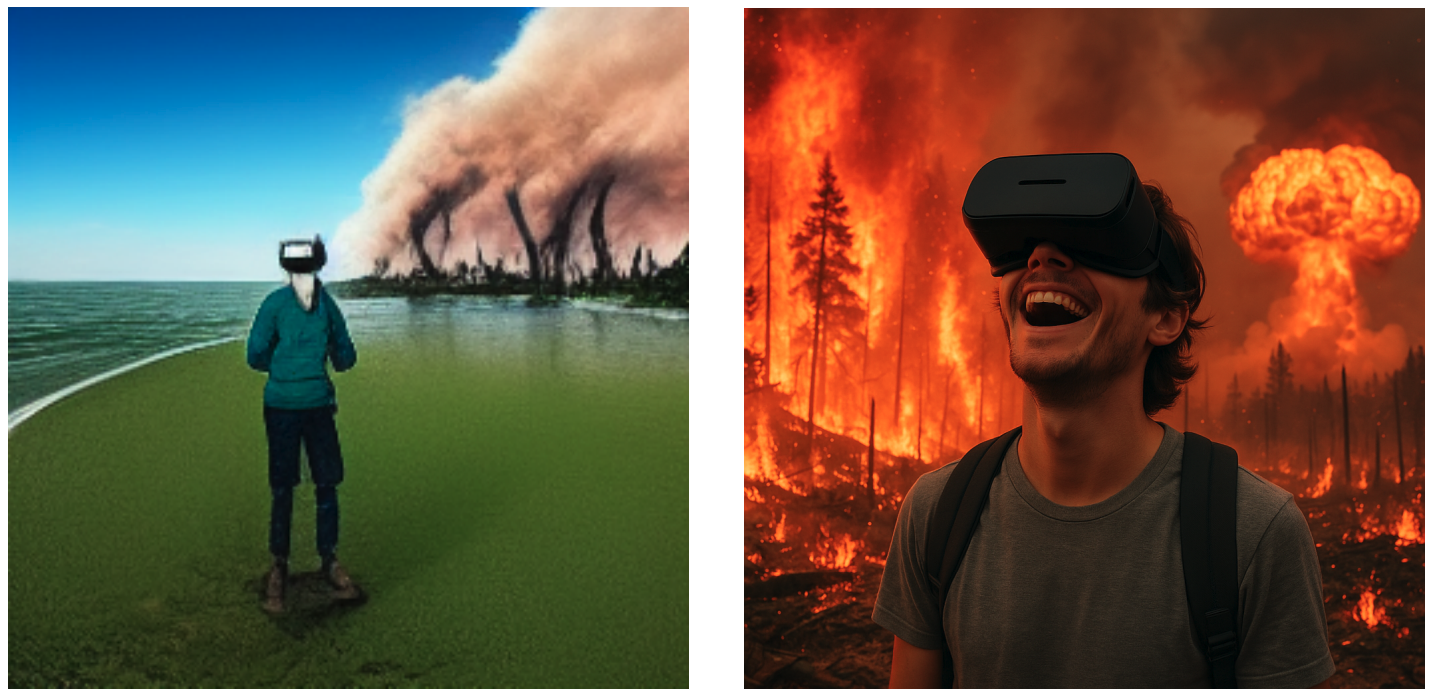
\includegraphics[width=1\linewidth]{comparisonimages.png}
    \caption{An illustration of the rapid developments in generative AI that took place in the time period spanning this thesis. \textbf{Left:} generated by the author in June 2022 using the prompt: "A person with a VR headset in the middle of an ecological catastrophe". \textbf{Right:} generated by the author exactly three years later, in June 2025.}
    \label{fig:enter-label}
\end{figure}

These technologies have not stayed in the lab; increasingly, they are becoming widely adopted and a part of everyday life for millions of people. A report by the UBS firm estimated ChatGPT reached 100 million users two-months after launch, making it the fastest application to reach this milestone \cite{Hu2023-ie}. Today, educators employ tools like ChatGPT and other chatbots to develop lesson plans, students leverage it for essay writing, doctors are using it to generate discharge summaries \cite{Patel2023-fg}, researchers use it to locate scholarly information and draft manuscripts, programmers are using it to write code, and laypeople are using it to ask questions, brainstorm ideas, write emails, among many other uses. 

Image-generation tools such as Leonardo, MidJourney, DALL-E, and Stable Diffusion have garnered significant user bases. According to a recent survey by Adobe (2024), approximately 40\% of designers have incorporated some form of generative AI into their design processes \cite{Offerman2024-lf}. People use these tools to create art, ideate designs, reimagine interior designs, create materials for presentations and more. 

As capabilities and adoption rise, AI is poised to become one of the most transformative technologies in modern history. Among the many questions raised by these developments, including ethical, political, economic, and environmental, one of the central ones is: How will generative artificial intelligence influence and intersect with human creativity, and how can we leverage it effectively while maintaining creative agency?

\subsection{Creativity, Technology and Artificial Intelligence}

Historically, technology and creativity have co-evolved in complex and intertwined ways. Almost all human creative activities rely on tools, and new technologies invariably open up novel creative possibilities and practices. However, new technologies can also lead to the automation of part of the creative process and in some cases, the replacement of human creators.

The invention of the camera provides an illustrative example. As a technology, the camera was initially partly met with resistance. The French poet Baudelaire famously argued that the purely material applications of photography would be detrimental for art \cite{Baudelaire1955-ae}, and art critics and theorists criticised the effect of the mechanisation of visual production such as in Walter Benjamin's famous essay The Work of Art in the Age of Mechanical Reproduction \cite{Benjamin1935-wd} . Photography did indeed supplant some traditional painting practices. Hand-painted magazine illustrations and commercial art, once a vital source of income for artists like Magritte in the early stages of their careers, are now predominantly produced through photography and digital methods. 

However, the camera also expanded creative possibilities by enabling the rise of photography and later film as rich new artistic practices in their own right. In a more nuanced way, photography influenced painting, and painting influenced photography, pushing each other in new directions . In his book "Art and Photography", Aaron Sharf discussed the mutual artistic influence of photography and painting, and described how the camera led to painters to reconsider and develop their techniques by providing them with new perspectives and reference material \cite{Scharf1968-na}. The rise of Impressionism, can be, at least to some degree, understood as the practice of painting occupying a less literal niche to visually capture reality. For Vincent Van Gogh, the advantage of Impressionism was that it provided "a deeper resemblance than the photograph" \citep[p. 116]{Marmor1997-ka} and for photographer Henry Peach Robinson, Impressionism did good to photography by showing "we should represent what we see, and not what the lens sees" \citep[p. 87]{Robinson1896-mo}. 

Artificial intelligence may interact with human creative practices in similar ways. It may automate some creative practices completely, support existing ones, and become a tool for new creative practices altogether. In this thesis, I am concerned with a distinct possibility that may integrate aspects of all them but also open new avenues for the co-evolution of creativity and technology: that of \textit{\textbf{co-creativity}}. In co-creative interactions, the technology itself exhibits creative capacities and is able to collaborate synergistically with human creators.

\subsection{Human-AI Co-Creativity}

Candy \cite{Candy2002-ra} described \textit{co-creativity} between people as a closely woven interaction that produces an output as a result of a symbiotic combination of actions. Creative participants align goals and intentions, collaboratively moving towards an outcome. In recent years, the field studying the potential for co-creativity between humans and machines has grown. 

Davis \cite{Davis2013-jy} first introduced the concept of human-computer co-creativity, describing an interaction where the computer is not just a rigid executor but adapts dynamically, drawing on computational creativity algorithms to respond to the user. Since then, across a growing literature, authors argue for the potential of human-AI co-creativity as a scenario that can augment, enhance and support human creativity, mitigating many of the risks posed by this technology while unlocking the beneficial opportunities it provides.  \cite{Yannakakis2014-zs,Kantosalo2020-zf,Rezwana2022-gg,Moruzzi2024-cq,Haase2024-yp,Lin2023-zq,Karimi2018-wi,Vinchon2023-gh}. Various definitions have been proposed for human-AI co-creativity. Drawing from them, I provide the following definition in my own terms to be be used throughout this thesis: 

\begin{quote}
\emph{A type of human-AI interaction involving creative contributions from both human and AI and where the outputs cannot be uniquely attributed to the creative behaviour of one them.}
\end{quote}


This choice in definition and term usage of "creative contributions" and "creative behaviour" is motivated by three main characterisations in the literature of human and machine creativity. 

First, by the widely accepted characterisation of something as creative if it is both \textbf{novel (or surprising)} and \textbf{valuable (or appropriate)} \cite{Amabile1983-lj, Sternberg1998-oz, Runco2012-mk, Boden2003-hk}. As such, I refer to a \textit{creative contribution} as one that satisfies this double constraint, and \textit{creative behaviour} as a process that can produce it. 

Acknowledging that novelty and value depend on frames of reference, my own definition of co-creativity considers the working definition of computational creativity offered by Colton and Wiggins' \cite{Colton2021-bt} as observer dependent.  They define computational creativity as:

\begin{quote}
The philosophy, science and engineering of computational systems which, by taking on particular responsibilities, exhibit behaviours that unbiased observers would deem to be creative.
\end{quote}
 
Thirdly, I draw from Rhodes' \cite{Rhodes1961-od} 4P's of creativity, which later Jordanous re-conceptualised for computational creativity \cite{Jordanous2016-xb} and which I here defined in my own terms: 

\begin{itemize}
    \item Person/Producer: The features of the system that make it capable of a particular creative behaviour and contributions.
    \item Process: The methods, strategies and algorithms used to drive creative behaviour and contributions.
    \item Press: The environment environment in which a generative system acts, including its interaction with the user and influences its creative behaviour and contributions.
    \item Product: The outputs produced from the interactions between the above resulting in creative behaviour and contributions.
\end{itemize}

Lastly, my understanding of creativity is heavily informed by Bown's notion of distributed creativity, as a process not exclusive to humans, which can be observed in natural and artificial systems (individual and collective), and which considers creativity as emerging from interactions within networks of distributed agency rather than emanating from individuals \cite{Bown2012-gg, Bown2021-os}. 

As such, human-AI co-creativity is a type of emergent and relational creativity, which, as other authors have suggested, can be attributed not to any of the agents but rather to the ensemble of interacting agents as a whole \cite{Davis2013-jy, Rezwana2023-rt}

\subsubsection{Machine Creativity?}

Through his concept of Material Agency, Lambros Malafouris argues that a craftsman is influenced by his tools and materials as much as he is influenced by them \cite{Malafouris2013-by}. This idea similarly underpins the concepts of Extended Cognition and Extended Mind Theories, both highly influential in creativity studies and which posits that tools and environments are extensions of a person's mind. A natural question arises then: how is the emergent co-creativity of a human-AI interaction different from that of a person creating with their tools in a mutually influencing loop? Crucially, the difference is that in this case, the tool is capable of creative behaviour itself. According to the definitions of creative behaviour provided above, it becomes increasingly evident that this is the case. 

Achieving creative behaviour was an explicit goal of the founding project that first coined the term and defined the field of artificial intelligence: the Dartmouth Summer Research Project on Artificial Intelligence \cite{McCarthy1955-ls}. Since then,  many researchers have sought to describe how computers could act creatively and how this creativity can be measured \cite{Boden2003-hk, Boden1998-yn, Colton2012-jc, Bown2012-gg, Moruzzi2020-mw, Wiggins2006-zd, Jordanous2012-kw}. However, machine creativity has long been considered one of the final frontiers in artificial intelligence \cite{Colton2021-bt},

In 2016, AlphaGo decisively beat the top human player in the world of Go. Throughout this match, AlphaGo was observed to play highly unexpected but effective moves, thus satisfying the constraint for novelty and value. One example is the now famous \textbf{move 37}, an extremely unexpected move made by AlphaGo that ended up turning the game in its favour. One commentator narrating the game described it as "a very strange move," while another claimed he thought it was a mistake. After the move materialised its game-defining value, another commentator claimed: "It’s not a human move. I’ve never seen a human play this move. So beautiful."

While AlphaGo first learned from human match data, its success resided in a step of reinforcement learning, where it played against itself. This helped it identify moves that could be successful even if never played by a human. It was this how it arrived to the game defining move 37, which was calculated to have 1 in 10,000 chance of being played by a human in that situation. A common counterargument to the possibility of AI creativity is that these algorithms only learn from human data and thus can only produce outputs that plausible replicate them. However, the AlphaGo example showcases the possibility of behaviour in machines that produce surprising, novel an valuable outputs \textit{and} that are highly different from that which a human would do.

Today, advances in generative AI reinforce the possibility of creative behaviour in other fields. As mentioned above, LLMs have now outperformed humans in some standardised tests of creativity and divergent thinking, such as the Alternative Uses Test and Torrance Test, in some case scoring in the top 1\% for originality and fluency \cite{Hubert2024-kv, Guzik2023-cl, Koivisto2023-lw}. Turing-style tests have shown humans have a hard time distinguishing art generated with AI and art generated by humans \cite{Alexander2024-pz}. 

While this may paint primarily a future of displacement of human creativity by automated means, the emergence of machine creative behaviour has also begun to opens the possibility for machine creativity that helps expand human creativity and synergise with it. 

\subsection{The case for human-AI co-creativity}

While AlphaGo decisively defeated the top human player in the world exhibiting moves that could be deemed creative, Metz \cite{Metz2016-dm} reported how AlphaGo has itself helped Go players see the game differently and improve as a result. In the field of creative writing, a study by Hitsuwari \cite{Hitsuwari2023-tw} showed that Haikus written in close cycles of iteration between humans and AI were rated higher than either writing Haikus alone. Increasingly, a growing creative artistic practice, including my own, has seen artists engaging AI technologies in co-creative ways, and using them to enable new previously unfeasible possibilities. 

Recent evidence suggests that beneficial outcomes are achieved when humans and AI are engaged in close cycles of collaboration and interaction, as opposed to each solving problems that require creativity on their own. A systematic study published in Nature by \cite{Vaccaro2024-ne} found evidence for what they term "human-AI synergy", measured as greater performance of Human and AI compared to Human or AI acting alone in the field of content production. A study done in collaboration between Harvard Business School and international consulting firm Boston Consulting Group looked at the effect of 758 consultants leveraging LLMs. They found that close synergies between humans and LLMs led to the highest outcomes compared to humans alone and to humans simply outsourcing tasks to the LLM with minimal involvement \cite{DellAcqua2023-og}. In a similar finding, McGuire \cite{McGuire2024-im} showed that when humans assume more passive roles of outsourcing creative production in  the case of writing, creative self efficacy and feelings of agency diminish, but when the interface facilitates them engaging as active co-creators, their creative self efficacy improves, as well as the measured outcomes. 

However, enabling such co-creative interactions is not trivial, and many challenges lie ahead. 

\subsection{Problem Statement: The Challenges of Human-AI Co-creativity}

With this, we arrive at the problem definition, which presents the central challenge in designing effective co-creative AI and which represent the central challenge addressed in this thesis. Broadly, it can be divided in two: challenges concerning the human user, and those concerning the co-creative system itself itself.

\subsubsection{Human Side}

Humans often over-rely on automated systems, leading to \textbf{minimal involvement} and, ultimately, a loss of skill and agency. In a study by Gerlich \cite{Gerlich2025-as} involving 666 participants, increased use of language models correlated with decreased critical thinking skills, apparently due to cognitive offloading. Similarly, a study by Carnegie Mellon and Microsoft Research found \cite{Lee2025-dw} that higher confidence in generative AI correlated with decreased measures of self-critical thinking. Conversely, another large-scale study by Essel et al. \cite{Essel2024-qc} reported the opposite effect in a controlled setting: students who engaged with a chat-based language model, and who received a pre-written set of prompts designed to stimulate critical reflection with the model, showed greater measures of critical and creative thinking.

These conflicting findings suggest that outcomes depend heavily on \emph{how} users interact with AI, which can be shaped by interface and interaction design but also personal motivations and context \cite{Lehmann2022-kr, Kantosalo2020-nh,Liapis2016-bv,Lin2023-jd,Karimi2020-cf,Moruzzi2024-cq, Rezwana2022-gg,Abbas2024-sf}. For example, while trust in the AI system can lead to greater overreliance, research shows that trust is important for effective co-creation \cite{McCormack2019-yh, Louie2020-aq, Kruger2017-xa, McCormack2020-ix, Hutchings2020-bv, Wang2020-cw, Rezwana2022-ui}. 

These nuances and potential contradictions highlight how it remains unclear how best to design systems and interfaces to foster active user engagement and co-creativity. 

\subsubsection{AI Side}
Generative AI systems themselves also pose several challenges for co-creativity. Chief among these are difficulties in controlling and steering outputs—leading some practitioners to describe them as “slot machines” \cite{Nebelong2023-rb}—and a lack of support for the iterative, evolving nature of the creative process \cite{Park2024-gw}. Moreover, they are often viewed as “black boxes” with low interpretability \cite{Llano2022-ti, El-Assady2022-qc}, can produce overly generic outputs that some practitioners feel lack a “human touch” \cite{Park2024-gw}, and may override or overwrite user-created content in undesirable ways \cite{Buschek2021-ks}.

In addition, while forming mutual understanding is crucial in collaboration and creativity, generative systems often struggle to grasp nuanced human goals \cite{Bown2024-yx}. Furthermore, in human–human co-creative scenarios, collaborators can challenge one another and offer perspective shifts that drive the creative process forward. By contrast, generative systems are typically trained to strictly follow user instructions \cite{OpenAI2022-pj} or user prompts \cite{Ramesh2022-kc}, limiting their potential to help users explore genuinely novel or unexpected directions \cite{Buschek2021-ks }.

These challenges are multi-faceted and can be approached from various angles. In this thesis, they are examined through the lens of interaction design and practice-based research. 

\section{Approach}

\subsection{Hypothesis}

To address the previously highlighted challenges, I began with the hypothesis that \emph{dialogic interaction} can mitigate many of these limitations. This hypothesis is informed by the observation that traditional interactions with computers, including generative systems, typically follow a linear pattern in which a command is given and an output is returned (see Figure \ref{fig:unidirectional}). 

\begin{figure}[hbt!]
    \centering
    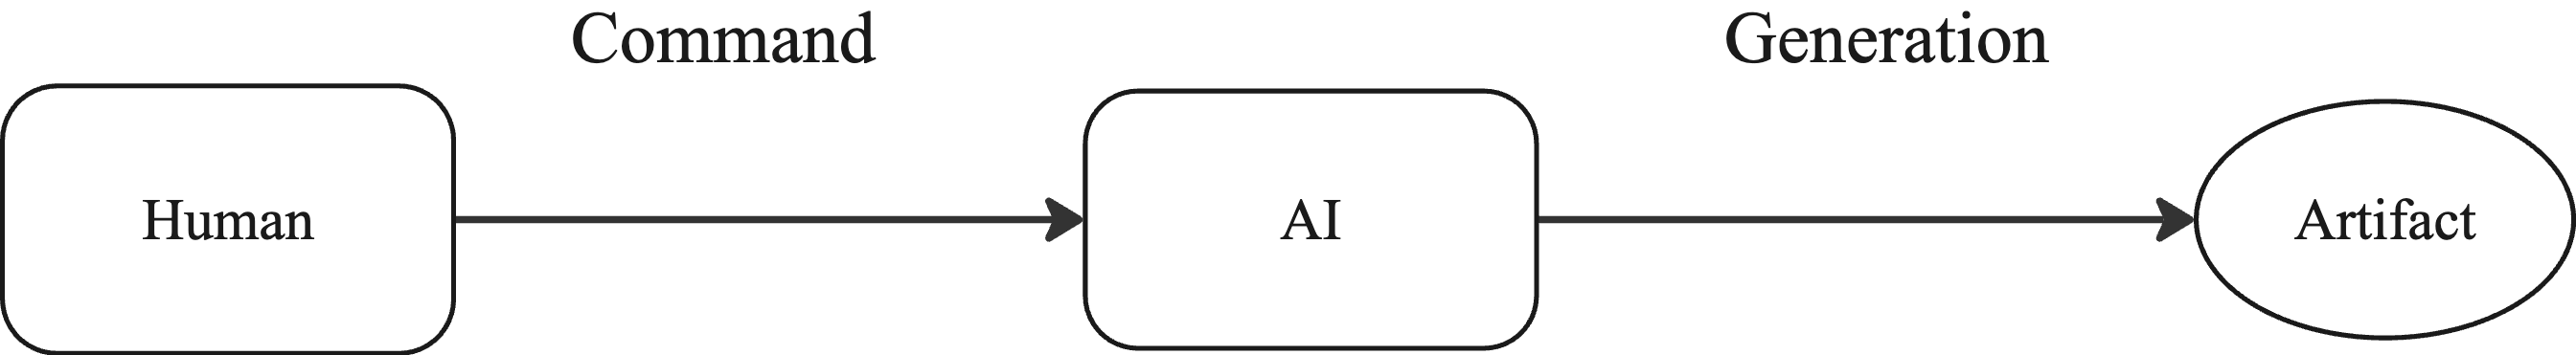
\includegraphics[width=0.75\linewidth]{unidirectional.png}
    \caption{Example of an unidirectional interaction with a generative AI system}
    \label{fig:unidirectional}
\end{figure}

However, as computers increasingly exhibit creative potential, the conventional command--execute paradigm becomes insufficient for fostering collaborative relationships. Instead, effective \emph{co-creative} engagement calls for \emph{dynamic back-and-forth conversations}, wherein both human and AI agents participate in iterative cycles of mutual understanding and influence. This is what I refer to by dialogic interaction. Importantly, in a dialogic process, participants can communicate \emph{both through} the creation itself and \emph{about} the creation (see Figure \ref{fig:dialogicthroughandabout}), thereby enabling deeper collaboration. As such, conversation may be a part of it, but not the exclusive component. 

\begin{figure}
    \centering
    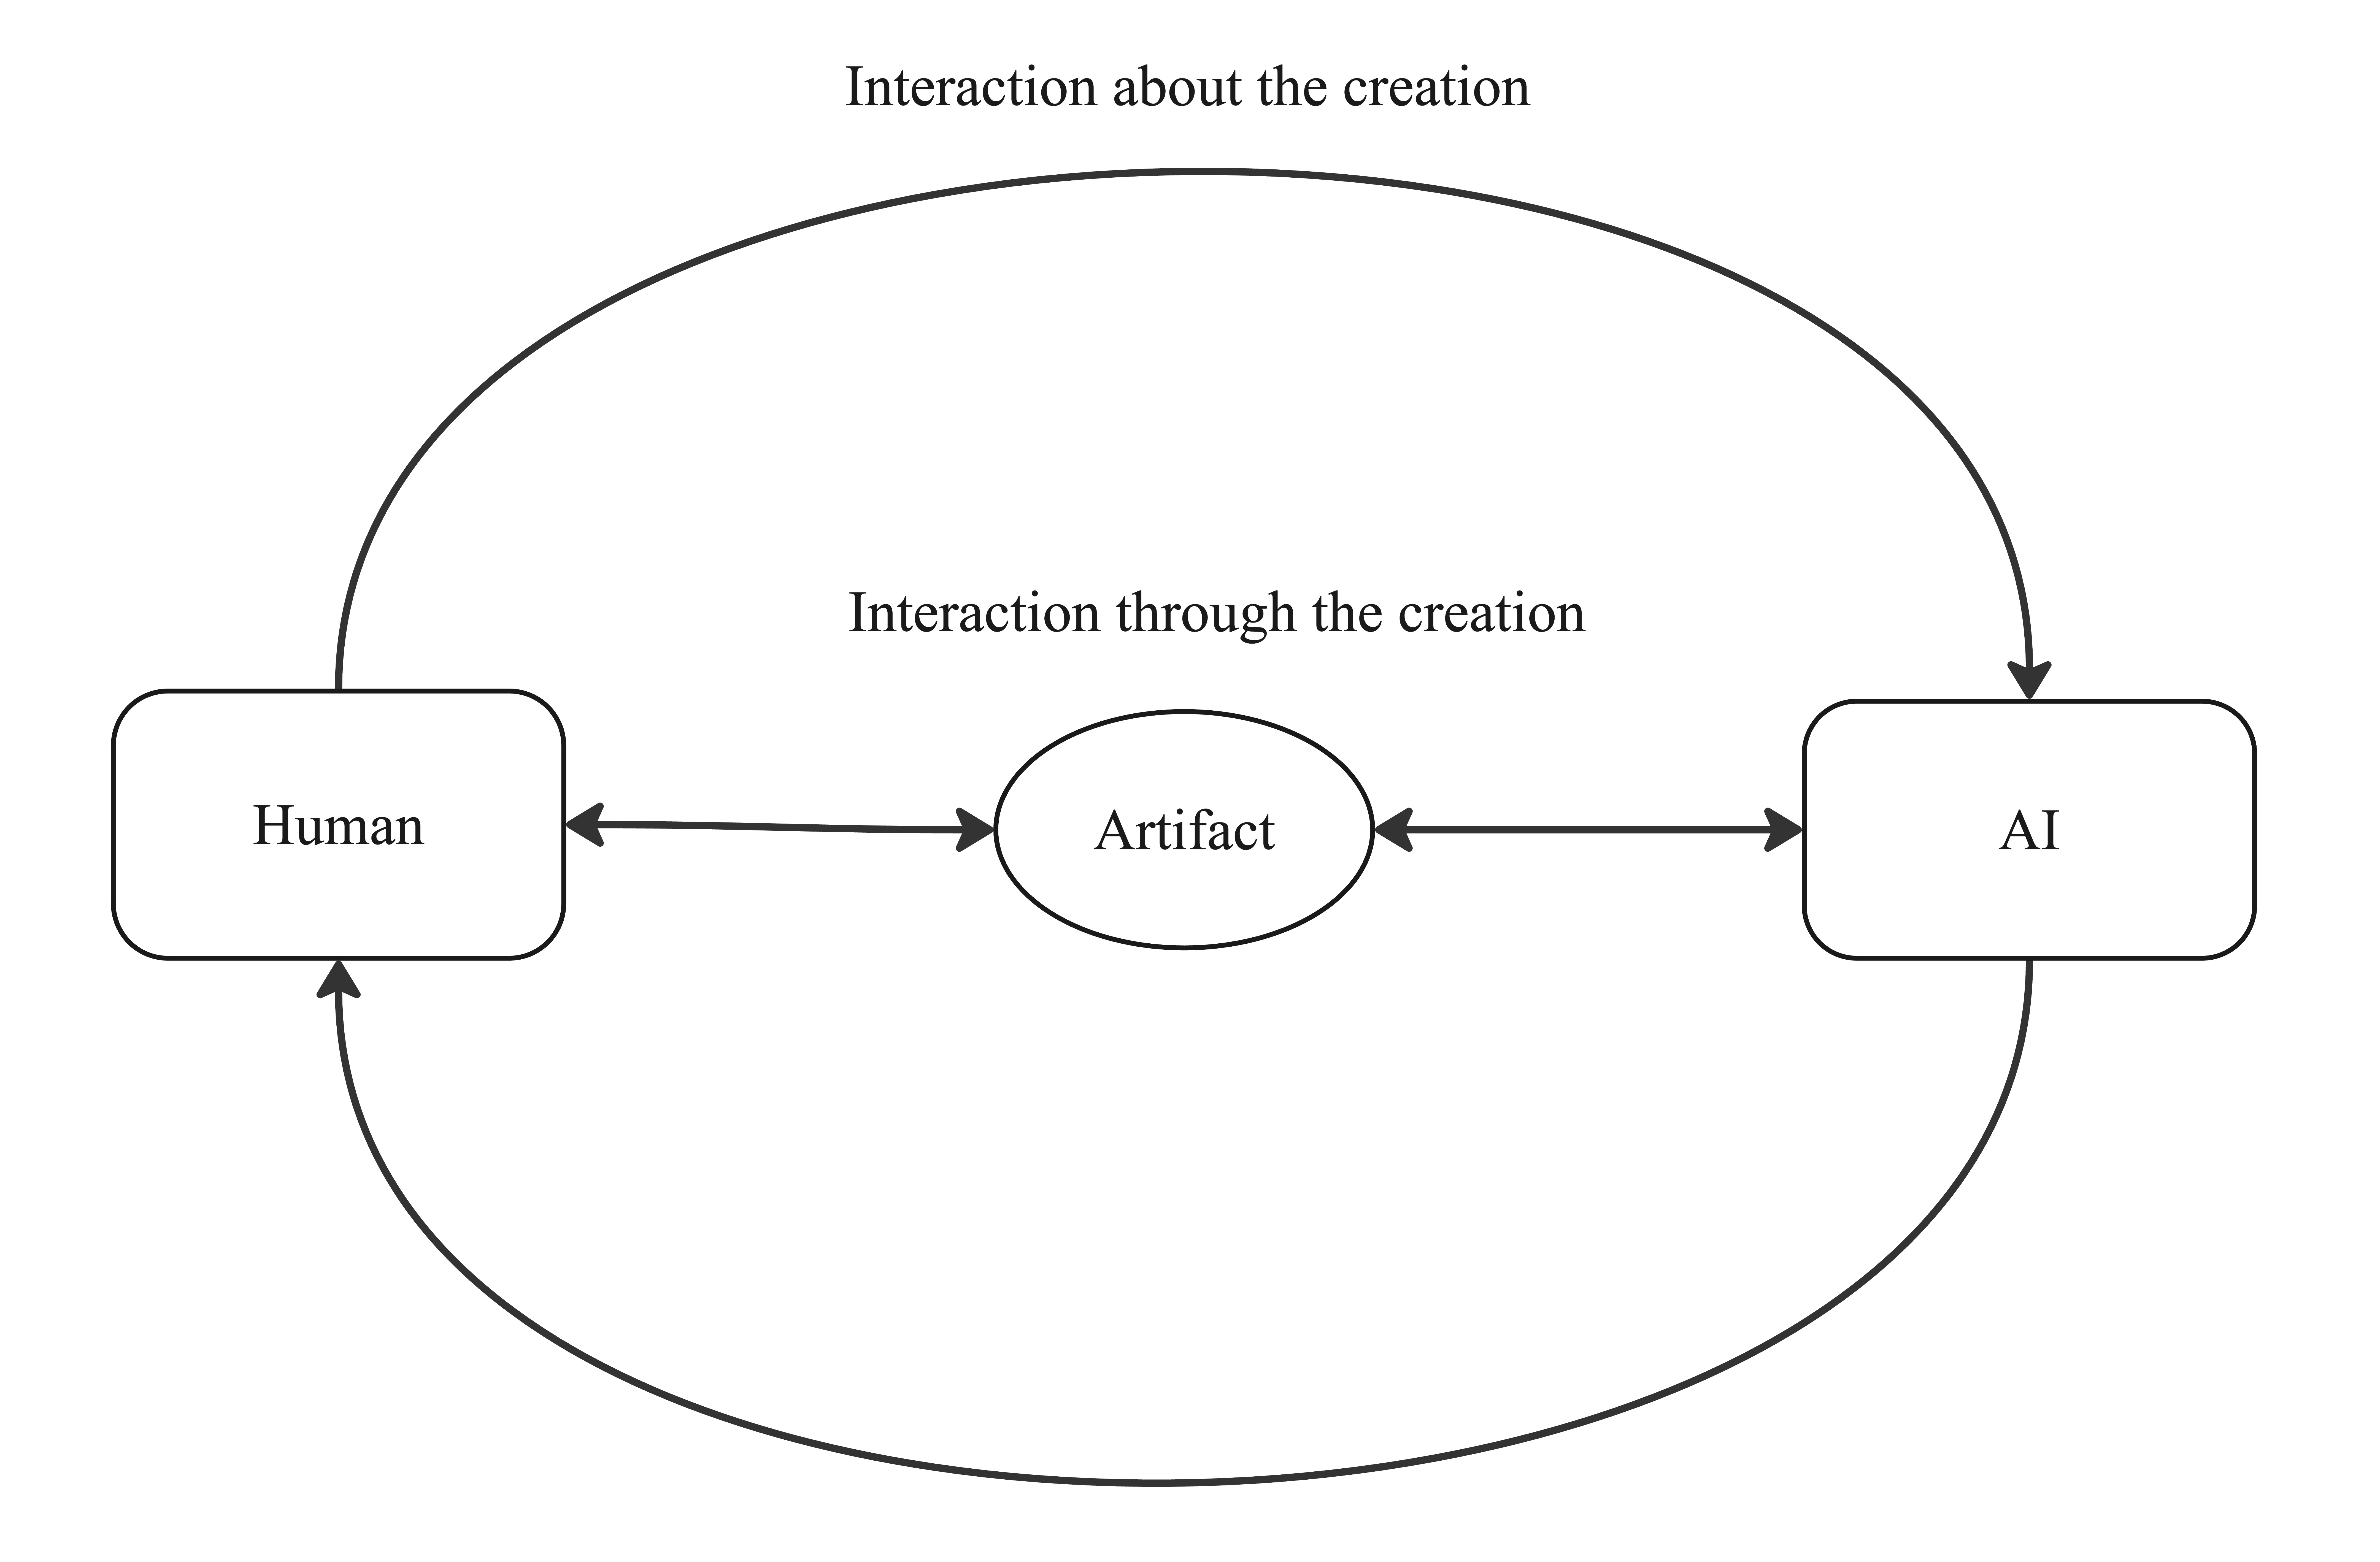
\includegraphics[width=0.75\linewidth]{dialogicthroughandabout.jpg}
    \caption{Diagram showing a dialogic interaction between a human and generative AI system interacting through and about the creation}
    \label{fig:dialogicthroughandabout}
\end{figure}

Dialogue has long been discussed in fields such as Human--Computer Interaction (HCI) and creative practice as a means to model interactions with computers and creative tools. Despite this, it remains underformalized as an interaction design concept in HCI. My research, conducted as part of an Australian Research Council (ARC)-funded project exploring Dialogic Creative AI, builds on initial work by Grace and Bown to address this gap.

In light of the emergence of chat-based interfaces as the predominant mode of interaction with language models, it might seem self-evident that dialogic interaction can enhance co-creativity. However, my characterization of dialogue extends beyond bidirectional text exchanges. By drawing on philosophical, educational, and interdisciplinary dialogue literature, I develop a more comprehensive construct of \emph{dialogic interaction}---an original contribution to HCI---comprising six key elements:

\begin{itemize}
    \item Bidirectional communication
    \item Shared collaborative space
    \item Iteration
    \item Mutual Influence
    \item Mutual Understanding
    \item Context-awareness
\end{itemize}

These elements are discussed in detail in Chapter~3. Notably, while bidirectional textual exchanges (as exemplified by popular chat interfaces) constitute one component, my proposal predates the widespread adoption of chat-based interactions, including the late 2022 launch of ChatGPT. The public success of such interfaces underscores the value of \emph{one} aspect of dialogic interaction---namely, real-time two-way communication---yet many other elements remain to be explored. Throughout this thesis, I examine how these additional elements can further support effective human--AI co-creativity.

Against this backdrop, I formulated one overarching research question and three sub-questions to guide this inquiry:

\begin{quote}
\textbf{Core Research Question:}\\
\emph{How can we design generative AI systems that act as effective co-creators, maintaining human agency while effectively leveraging the creative potential of this technology?}
\end{quote}

\begin{quote}
\textbf{Sub-Questions:}
\begin{enumerate}
    \item \textbf{R1:} \emph{How does interaction design influence the role that humans and AI play in creative production?}
    \item \textbf{R2:} \emph{What is the potential of modelling dialogue in interaction design to enable effective human–AI co-creativity?}
    \item \textbf{R3:} \emph{Which interaction design principles can guide the development of effective co-creative systems?}
\end{enumerate}
\end{quote>

\subsubsection{Methodology}
To address my research questions, I adopt a mixed-methodology approach integrating qualitative and quantitative research methods across two strands: interaction design research and creative-led practice.

I focus specifically on human–AI co-creativity within three creative domains: writing, image generation, and interactive new media music installations. On one hand, I develop prototypes that are tested with users to evaluate the potential of dialogic interaction in enabling human–AI co-creativity. On the other hand, I engage in a creative practice-led approach by developing interactive artworks and collaborating with professional creatives in the completion of projects leveraging generative AI, which I then analyse as case studies. Through this analysis, I discuss both the potential and the limitations of these systems to be co-creative in real-world scenarios, with particular emphasis on dialogic interaction as a lens of analysis.

A diagram illustrating the approach and methodology is shown in \ref{fig:approach_figure}.

\begin{figure}[hbt!]
    \centering
    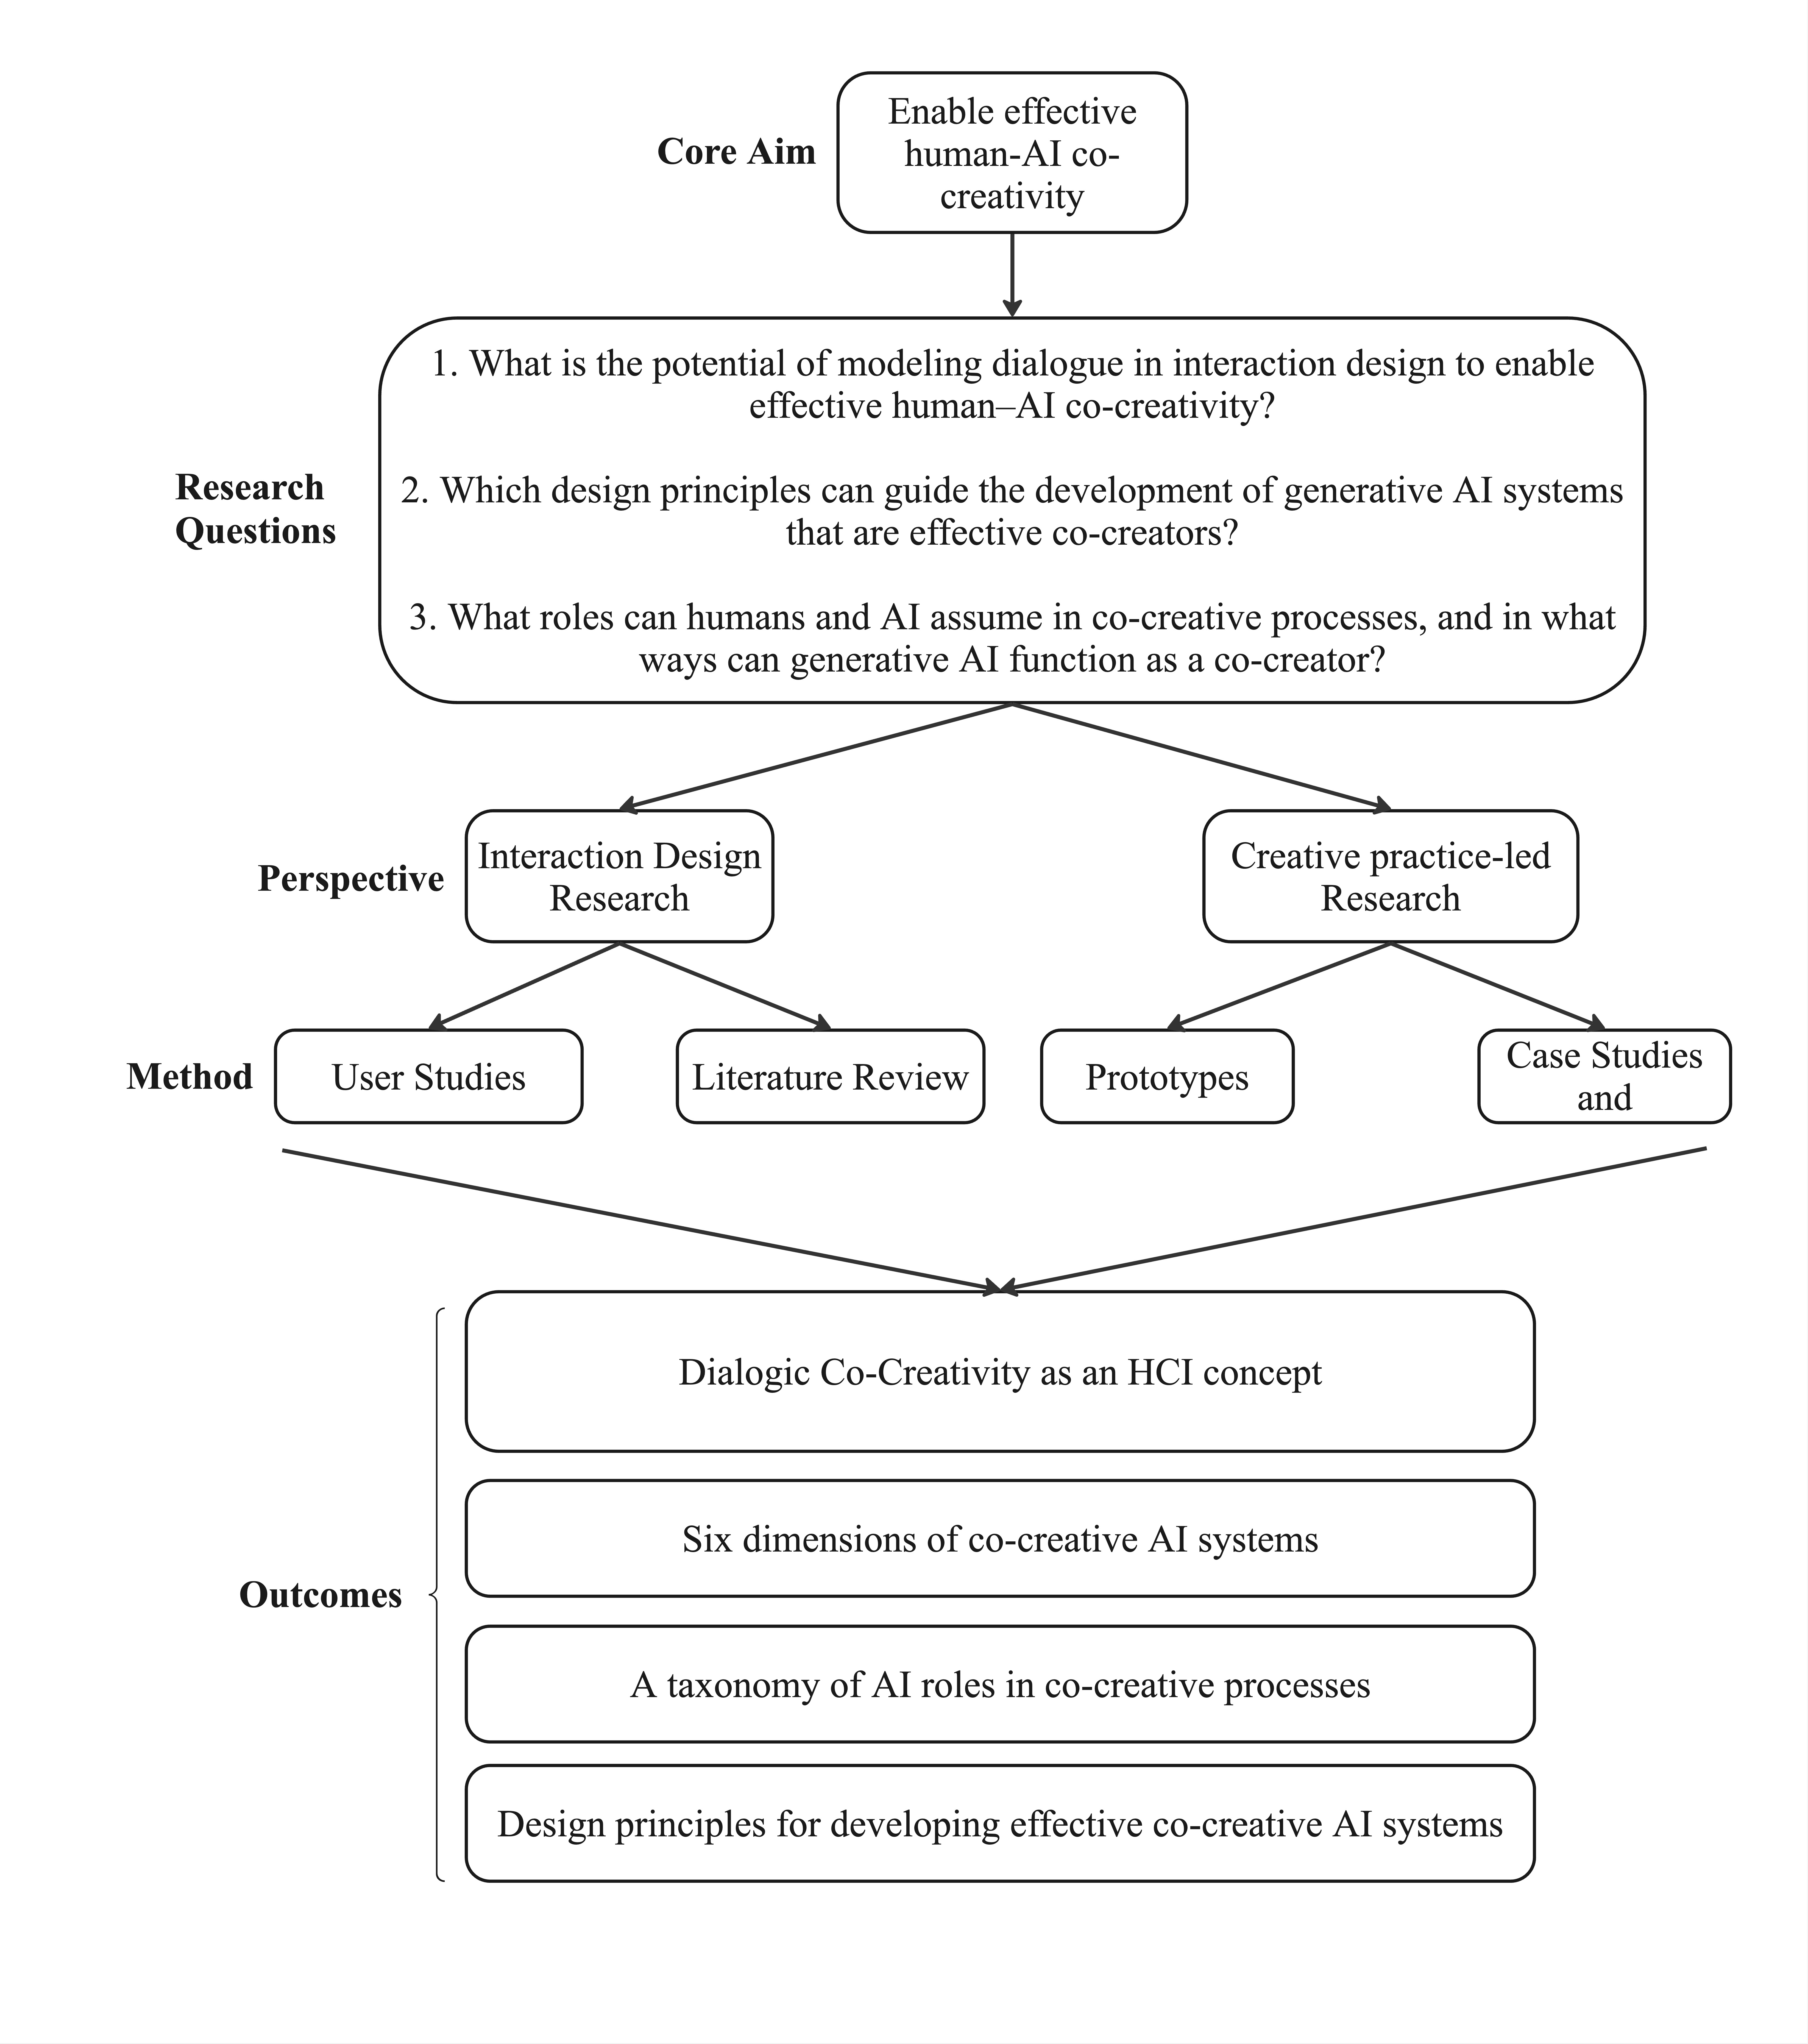
\includegraphics[width=1\linewidth]{Intro - Frame 1 (2).jpg}
    \caption{Diagram illustrating the approach followed to address the core research aim}
    \label{fig:approach_figure}
\end{figure}

\clearpage

\section*{Thesis Structure}

This thesis is structured chronologically but not strictly so, as I also prioritised grouping studies by creative practice: writing, image generation, and interactive sonic art installations. As such, the three primary study chapters—Chapters 4, 5, and 6—are organised accordingly. The preceding chapters establish the theoretical foundations that underpin the thesis, while the final chapter (Chapter 7) integrates the findings and conclusions.

\subsection*{Chapter 2: Literature Review}

Chapter 2 provides a literature review, contextualising the research within the broader field. It begins with an overview of state-of-the-art developments and recent progress in generative AI, establishing the technological landscape and its fundamental capabilities and limitations. The chapter then reviews key literature in computational creativity and human-AI co-creativity, followed by a discussion of dialogue as a relevant concept in interaction design. Although some aspects of dialogue are covered here, a more detailed exploration is presented in a dedicated chapter. The final section of Chapter 2 examines related approaches that apply dialogue as an interaction design concept in human-computer co-creativity.

\subsection*{Chapter 3: Conceptual Foundations of Dialogic Co-creativity}

Chapter 3 lays the conceptual foundations for dialogic co-creativity as an interaction design framework within Human-Computer Interaction (HCI). This chapter consists of two parts. 

\subsubsection{Preliminary Framework for Dialogic Co-creativity: } The first part includes a paper presented at the CHI Workshop on Generative AI (2022), where I introduced a preliminary framework for dialogic interaction. This early work explored bidirectional communication with language models in creative contexts. At the time, chat-based interfaces were not the dominant interaction paradigm for language models; most interactions were based on autocomplete or linear instructions. Through prompt engineering, we investigated the feasibility of engaging with AI in conversational creative dialogue, interacting both through and about the creation. This introduced distinction—interaction *through* versus *about*—became a central theme of dialogic interaction throughout the thesis.

\subsubsection{Six elements of dialogic co-creativity:} The second part of Chapter 3 was developed towards the later stages of my research and presents a more formalised definition of dialogic interaction. This definition is articulated through six key elements:

\begin{enumerate}[label=\arabic*.]
    \item Bidirectional Communication
    \item Shared Space
    \item Iteration
    \item Mutual Influence
    \item Mutual Understanding
    \item Context-Awareness
\end{enumerate}

These elements serve as the foundation for analysing and designing co-creative systems that facilitate human-AI collaboration.

\subsection*{Chapter 4: Co-Creative Writing}

Chapter 4 explores co-creative writing through two case studies. 

\subsubsection{Narrative Device: } The first part examines \textbf{Narrative Device}, an early prototype developed in late 2021 and early 2022. This prototype allowed users to input two distinct concepts, which a language model then combined to generate short stories, drawing on Boden’s concept of combinatorial creativity. The system, which was publicly released and gained viral popularity, facilitated the creation of over two million stories by more than a hundred-thousand users. For many users, this was their first experience of co-creating with a highly capable AI system.

On one hand, Narrative Device required users to engage in creative ideation by choosing concepts that, when combined, would produce an interesting or humorous story. On the other hand, the creative potential of AI was drawn to integrate these elements coherently and surprisingly (following the constraint of both novelty or surprise and value). While the system was positively received and users expressed satisfaction with it, a fundamental challenge was that, it did not allow users to iterate or refine the generated stories. This lack of \textbf{iteration} is an element of dialogic interaction and a common limitation expressed by users of this and other systems. This limitation stemmed in part from the fact that the underlying model (InstructGPT) was designed primarily for instruction-following rather than conversational interaction.

Following the release of ChatGPT in late 2022, chat-based conversational interfaces became the dominant paradigm for AI-assisted writing. While this bidirectional communication mode enabled greater iterative collaboration, I observed that it was limited for co-creativity as it primarily facilitated interaction *about* the creation rather than *through* it. This shift often leads users to assume an outsourcer role, delegating writing tasks to the AI rather than engaging in co-creation. Research suggests that this tendency can negatively impact users’ creative agency, self-efficacy, and involvement, and that interface design can mitigate this effect by encouraging deeper engagement \cite{Kantosalo2016-hg, McGuire2024-im}.

\subsubsection{From Instructors to Co-Authors: Mitigating Overreliance on AI Through Collaborative Writing Interfaces (manuscript submitted to ICCC 2025)} To address these challenges, I developed a second prototype in two iterations across 2023 and 2024. These prototypes introduced a collaborative text editor, enabling both human and AI to read and modify the text, alongside a chat window for discussing writing goals and making requests. This design allowed users to interact with the AI both through and *about* the creative process. 

Two user studies were conducted to evaluate this prototype. Unlike \textit{Narrative Device}, these studies were controlled and not publicly released. Although the participant sample was limited, they highlighted the potential of this interface to enhance human involvement. In the chat-only condition, users were more likely to agree that the AI had done most of the work. In contrast, in the shared editor condition, users reported contributing more of their own writing and assuming more active roles as co-creators. The development of these prototypes anticipated industry trends: a few months after these prototypes were developed, commercial AI tools integrated similar collaborative interfaces. For instance, Anthropic’s Claude introduced Artifacts in August 2024, followed by OpenAI’s Canvas for ChatGPT in October 2024. These developments reinforce the importance of integrating collaborative workspaces with chat-based interactions for human-AI co-creativity.

\subsection{Chapter 5: Interactive Sonic Art Installations}

Chapter 5 is comprised of two papers, each describing an interactive sonic art installations developed over two years. These installations primarily explored the dialogic co-creativity element of context-awareness, such that generative AI can act as a co-creator within a context, taking actions that affect that context, while maintaining human compositional and creative intent. 

Both of these installations were data sonificiation installations where an LLM was used a semantic interpretive bridge between data and and a generative soundscape. 

\subsubsection{Using GPT-3 to Achieve Semantically Relevant Data Sonificiation for an Art Installation: } This paper, presented at EvoMusArt 2023 in Brno Czech Republic, describes an installation commissioned by the Australian National University School of Cybernetics and developed in collaboration with Uncanny Valley, was presented at the Cybernetic Serendipity festival. The goal was to transform both the built and natural environment surrounding the festival into a dynamic soundscape. Live data streams—including global CO$_2$ levels, national economic indicators, and local weather conditions—were interpreted by a language model, which generated succinct textual descriptions. These descriptions were then converted into word embeddings and mapped onto a latent space of musical descriptors, creating a continuously evolving soundscape.

\subsubsection{Interpretative Data Sonification: Using LLMs to Interpret Data and Generate Continuous Soundscapes at the Sydney Opera House} This paper, presented at the Sound and Music Conference 2024 in Porto, Portugal describes a second installation, commissioned for the Sydney Opera House’s 50th anniversary, built upon this approach but with greater AI agency. Instead of merely interpreting data, the AI actively controlled aspects of the music generation process based on real-time environmental inputs, including building energy use, water consumption, and ongoing performances.

Through this installations, we showed the potential for large language models to understand and interpret complex structured and unstructured data, and then use those interpretations to drive a generative artwork. As such, becoming context-aware co-creators, that can act within it and take actions that affect it key element in dialogic interaction. 

However, both installations revealed challenges for this context to be acted upon effectively, particularly context window limitations and maintaining historical coherence over extended durations. The AI tended to fixate on certain patterns, limiting the generative scope. However, these works highlighted the potential of AI-mediated semantic interpretation in real-time reactive sound art, moving beyond direct data-to-sound mappings.

\subsection*{Chapter 6: Generative AI in Design and Media}

Chapter 6 presents two case studies exploring the co-creative potential of generative image and language models in visual domains, particularly focusing on the \textbf{iterative element of dialogic co-creativity}. 

\subsubsection*{AI-Assisted Interior and Furniture Design}

This project, in collaboration with Studio Snoop in Sydney, explored the use of AI in furniture and interior design. It resulted in an AI co-creator named *Tilly*, integrating a language model and a text-to-image model. The system was used to ideate and generate designs aligned with sustainability, natural materials, and human well-being. The project culminated in an installations at Milan Design Week where posters of the designs where shown. Attendees provided daily feedback to Tilly, an AI, which then informed design iterations by a team in Sydney.  This process culminated in a final design presentation at the end of the week.  Later that year, these designs were physically produced by artisans and studios worldwide and showcased at the London Design Festival. The project explored how generative AI can act as a co-creator, facilitating iterative, distributed creativity across time and space.

\subsubsection*{AI-Generated Portraits for the Australian Financial Review (AFR)}

This study, conducted with AFR Magazine, and presented at the 2024 International Conference on Computational Creativity (ICCC) in Jönköping, Sweden explored AI-generated portraits for their annual "Most Powerful People in Australia" feature. The goal was to create concept-driven images that reflected each subject’s personality and role. For example, the head of the Federal Reserve piloting a balloon as a metaphor for their control of inflation. The iterative collaboration between the AI system and human designers revealed challenges in controlling generative outputs and maintaining visual consistency. The publication of these AI-generated portraits sparked public debate, highlighting ongoing concerns about AI's role in creative industries.

\subsection*{Chapter 7: Conclusion}

The final chapter synthesises the findings from previous chapters and presents four key contributions:

\begin{enumerate}[label=\arabic*.]
    \item The potential of dialogic interaction to enable effective human-AI co-creativity.
    \item A novel characterization of six dimensions of co-creativity for designing generative AI systems.
    \item A taxonomy of AI roles in co-creative processes.
    \item A set of design principles for developing effective co-creative AI systems.
\end{enumerate}

These contributions provide insights for both researchers and practitioners in designing AI systems that foster meaningful human-AI collaboration.
    \chapter{Introduction}


\begin{flushleft}
\begin{minipage}[t]{0.80\textwidth}
\textit{It is true that there is no art without emotion\\
And there is no precision without craftsmanship\\
Just as there are no guitars without technology\\
Nylon technology for the high strings\\
Metal technology for the headstock\\
The press, the chisel, and the varnish\\
The carpenter's tools\\
The composer and his computer\\
The shepherd and his shaver\\
The alarm clock, announcing dawn\\
And in the telescope, the last star lingers\\
The machine is made by man\\
And it is what man makes of it}
\end{minipage}

\medskip
\hfill---Jorge Drexler, "Mi Guitarra y Vos"
\end{flushleft}

\bigskip

I vividly remember the first time I interacted with a language model. It was early 2019, and the model, GPT-2, was an early implementation of the novel transformer architecture leveraging the now-famous attention mechanism. It felt like a distinct experience. Back then, this model was open source, and to run it I had to download the model weights and scrape together a way to run it on a GPU, which I did with the help of a friend. It was not a particularly smooth experience, though it was exciting to be wrangling a neural network that somehow encoded the capability of producing language.

This model was rudimentary; when generating long sequences it often yielded nonsensical results and tended to go off in divergent directions. But it certainly had unprecedented language capabilities, sometimes generating text undistinguishable from that written by a person. This capacity, the ability to produce language, was previously thought exclusive to humans. Not anymore. Perhaps even more interestingly, interacting with these generative language systems often yielded genuinely interesting ideas \textit{in my own mind}.  The experience made me want to devote my work and research to the field of artificial intelligence and how humans can interact with it in creative and beneficial ways.

A few months later, in mid-2019, as I was applying to a master’s at the Australian National University’s 3A Institute to study the development of responsible AI-enabled systems, I decided to co-author my essay using GPT-2 as a "co-author", which proved both technically difficult and creatively rewarding. I wrote the first paragraph, which I fed to the model to generate the second paragraph, and so on. The topic was the potential implications of humans and AI interacting to co-create.

The whole process was disclosed and documented, and the code I used was provided with instructions on how to replicate exactly the text I generated. This was submitted alongside my essay, and a description of my iterative approach. Sometimes the paragraphs were not interesting, so I generated them again. At other times, they suggested ideas that opened up new possibilities, leading the essay in new directions. The most significant one was the suggestion, by the model, that \textit{language is the first technology}. Regardless of the anthropological validity of this claim, it made me reflect on the ironically profound implications of interacting with a technology that can produce language.

I eventually received an offer to the master’s and travelled from Mexico to Australia, arriving in early 2020, just a few weeks before the pandemic. After finishing my masters, I began this PhD research in late 2021 focused on enabling human-AI co-creativity. I finalised writing this thesis in early 2025. In that relatively short period, progress in AI accelerated rapidly. Generative AI, which only a few years ago consisted of rudimentary models mostly used by curious neural network wranglers like myself, are now commonplace, used by hundreds of millions of people.

These emerging generative capabilities, across not only language, but also music, images, videos, music, code, and more, raise many pressing ethical, philosophical, and economic questions. They also open up the possibility of human-AI co-creativity.

The PhD research presented in this thesis is concerned with this possibility. In particular, it explores how to design generative AI systems that function effectively as co-creators, augmenting human creativity and preserving user agency, while allowing users to harness the creative potential of these technologies. It is also a practice-led exploration, in which, through my own creative work, I explore the potential and limitations of generative artificial intelligence as a co-creator. 

\section{Background}

In the field of natural language generation, neural networks have evolved from producing short, minimally coherent text sequences \cite{Bengio2003-xn, Sutskever2011-ne, Graves2013-yv} to large language models (LLMs) capable of achieving near, at or past human-level performance on complex tasks \cite{Vaswani2017-pb, Brown2020-js, Thoppilan2022-jf, OpenAI2023-lt, Anthropic2024-tc, DeepSeek-AI2025-ai, Gemini-Team2024-wk}. Today, LLMs can generate entire essays, pass advanced academic examinations at the PhD level, write software code at or above human proficiency, compose whole-length novels, engage in multi-step reasoning, and understand and reason across images, audio, and video \cite{Gemini-Team2023-ux, OpenAI2024-em}. 

In terms of creative capabilities, a recent study by Hubert et al. reported that an LLM outperformed humans in standardised tests of creativity and divergent thinking \cite{Hubert2024-kv} while another study by Guzik et al \cite{Guzik2023-cl} reported that an LLM scored in the top 1\% for originality and fluency in the Torrance Test, a standardised assessment used to measure human creativity. 

The field of image generation has similarly made significant strides. Neural networks went from producing rudimentary images \cite{Goodfellow2014-jz, Mordvintsev2015-oz} to modern diffusion models capable of generating photorealistic images often indistinguishable from genuine photographs, and to produce images in a variety of artistic styles \cite{Ramesh2021-xb, Rombach2021-wf, Ho2020-zj, OpenAI2021-te, Nichol2021-ne, Zhang2023-by}. In a recent survey with more than 11,000 participants, humans were not reliably able to distinguish AI generated art from paintings made by humans. Moreover, participants tended to rate AI-images slightly higher in preference \cite{Alexander2024-pz}. Similar progress is evident in music generation, where AI has progressed from creating simple melodies \cite{Huang2018-pc, Dhariwal2020-au, Roberts2019-ym} to full-scale songs \cite{Copet2023-mh, Suno2024-wa, Udio2024-rc}. Currently, emerging video-generation models such as Gen3-Alpha, Sora, MovieGen suggest the extension of this trend to the moving image domain \cite{Runway2024-zs, Polyak2024-lh, OpenAI2024-ua}.

\begin{figure}
    \centering
    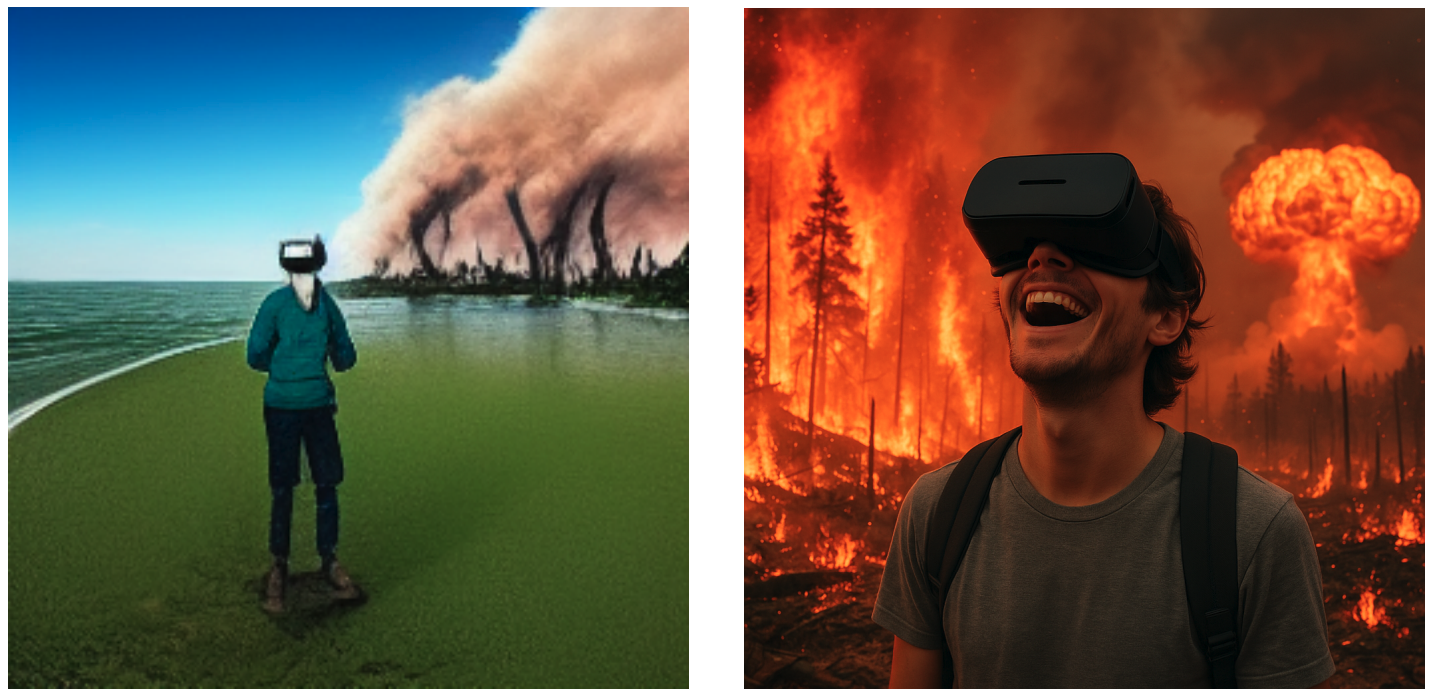
\includegraphics[width=1\linewidth]{comparisonimages.png}
    \caption{An illustration of the rapid developments in generative AI that took place in the time period spanning this thesis. \textbf{Left:} generated by the author in June 2022 using the prompt: "A person with a VR headset in the middle of an ecological catastrophe". \textbf{Right:} generated by the author exactly three years later, in June 2025.}
    \label{fig:enter-label}
\end{figure}

These technologies have not stayed in the lab; increasingly, they are becoming widely adopted and a part of everyday life for millions of people. A report by the UBS firm estimated ChatGPT reached 100 million users two-months after launch, making it the fastest application to reach this milestone \cite{Hu2023-ie}. Today, educators employ tools like ChatGPT and other chatbots to develop lesson plans, students leverage it for essay writing, doctors are using it to generate discharge summaries \cite{Patel2023-fg}, researchers use it to locate scholarly information and draft manuscripts, programmers are using it to write code, and laypeople are using it to ask questions, brainstorm ideas, write emails, among many other uses. 

Image-generation tools such as Leonardo, MidJourney, DALL-E, and Stable Diffusion have garnered significant user bases. According to a recent survey by Adobe (2024), approximately 40\% of designers have incorporated some form of generative AI into their design processes \cite{Offerman2024-lf}. People use these tools to create art, ideate designs, reimagine interior designs, create materials for presentations and more. 

As capabilities and adoption rise, AI is poised to become one of the most transformative technologies in modern history. Among the many questions raised by these developments, including ethical, political, economic, and environmental, one of the central ones is: How will generative artificial intelligence influence and intersect with human creativity, and how can we leverage it effectively while maintaining creative agency?

\subsection{Creativity, Technology and Artificial Intelligence}

Historically, technology and creativity have co-evolved in complex and intertwined ways. Almost all human creative activities rely on tools, and new technologies invariably open up novel creative possibilities and practices. However, new technologies can also lead to the automation of part of the creative process and in some cases, the replacement of human creators.

The invention of the camera provides an illustrative example. As a technology, the camera was initially partly met with resistance. The French poet Baudelaire famously argued that the purely material applications of photography would be detrimental for art \cite{Baudelaire1955-ae}, and art critics and theorists criticised the effect of the mechanisation of visual production such as in Walter Benjamin's famous essay The Work of Art in the Age of Mechanical Reproduction \cite{Benjamin1935-wd} . Photography did indeed supplant some traditional painting practices. Hand-painted magazine illustrations and commercial art, once a vital source of income for artists like Magritte in the early stages of their careers, are now predominantly produced through photography and digital methods. 

However, the camera also expanded creative possibilities by enabling the rise of photography and later film as rich new artistic practices in their own right. In a more nuanced way, photography influenced painting, and painting influenced photography, pushing each other in new directions . In his book "Art and Photography", Aaron Sharf discussed the mutual artistic influence of photography and painting, and described how the camera led to painters to reconsider and develop their techniques by providing them with new perspectives and reference material \cite{Scharf1968-na}. The rise of Impressionism, can be, at least to some degree, understood as the practice of painting occupying a less literal niche to visually capture reality. For Vincent Van Gogh, the advantage of Impressionism was that it provided "a deeper resemblance than the photograph" \citep[p. 116]{Marmor1997-ka} and for photographer Henry Peach Robinson, Impressionism did good to photography by showing "we should represent what we see, and not what the lens sees" \citep[p. 87]{Robinson1896-mo}. 

Artificial intelligence may interact with human creative practices in similar ways. It may automate some creative practices completely, support existing ones, and become a tool for new creative practices altogether. In this thesis, I am concerned with a distinct possibility that may integrate aspects of all them but also open new avenues for the co-evolution of creativity and technology: that of \textit{\textbf{co-creativity}}. In co-creative interactions, the technology itself exhibits creative capacities and is able to collaborate synergistically with human creators.

\subsection{Human-AI Co-Creativity}

Candy \cite{Candy2002-ra} described \textit{co-creativity} between people as a closely woven interaction that produces an output as a result of a symbiotic combination of actions. Creative participants align goals and intentions, collaboratively moving towards an outcome. In recent years, the field studying the potential for co-creativity between humans and machines has grown. 

Davis \cite{Davis2013-jy} first introduced the concept of human-computer co-creativity, describing an interaction where the computer is not just a rigid executor but adapts dynamically, drawing on computational creativity algorithms to respond to the user. Since then, across a growing literature, authors argue for the potential of human-AI co-creativity as a scenario that can augment, enhance and support human creativity, mitigating many of the risks posed by this technology while unlocking the beneficial opportunities it provides.  \cite{Yannakakis2014-zs,Kantosalo2020-zf,Rezwana2022-gg,Moruzzi2024-cq,Haase2024-yp,Lin2023-zq,Karimi2018-wi,Vinchon2023-gh}. Various definitions have been proposed for human-AI co-creativity. Drawing from them, I provide the following definition in my own terms to be be used throughout this thesis: 

\begin{quote}
\emph{A type of human-AI interaction involving creative contributions from both human and AI and where the outputs cannot be uniquely attributed to the creative behaviour of one them.}
\end{quote}


This choice in definition and term usage of "creative contributions" and "creative behaviour" is motivated by three main characterisations in the literature of human and machine creativity. 

First, by the widely accepted characterisation of something as creative if it is both \textbf{novel (or surprising)} and \textbf{valuable (or appropriate)} \cite{Amabile1983-lj, Sternberg1998-oz, Runco2012-mk, Boden2003-hk}. As such, I refer to a \textit{creative contribution} as one that satisfies this double constraint, and \textit{creative behaviour} as a process that can produce it. 

Acknowledging that novelty and value depend on frames of reference, my own definition of co-creativity considers the working definition of computational creativity offered by Colton and Wiggins' \cite{Colton2021-bt} as observer dependent.  They define computational creativity as:

\begin{quote}
The philosophy, science and engineering of computational systems which, by taking on particular responsibilities, exhibit behaviours that unbiased observers would deem to be creative.
\end{quote}
 
Thirdly, I draw from Rhodes' \cite{Rhodes1961-od} 4P's of creativity, which later Jordanous re-conceptualised for computational creativity \cite{Jordanous2016-xb} and which I here defined in my own terms: 

\begin{itemize}
    \item Person/Producer: The features of the system that make it capable of a particular creative behaviour and contributions.
    \item Process: The methods, strategies and algorithms used to drive creative behaviour and contributions.
    \item Press: The environment environment in which a generative system acts, including its interaction with the user and influences its creative behaviour and contributions.
    \item Product: The outputs produced from the interactions between the above resulting in creative behaviour and contributions.
\end{itemize}

Lastly, my understanding of creativity is heavily informed by Bown's notion of distributed creativity, as a process not exclusive to humans, which can be observed in natural and artificial systems (individual and collective), and which considers creativity as emerging from interactions within networks of distributed agency rather than emanating from individuals \cite{Bown2012-gg, Bown2021-os}. 

As such, human-AI co-creativity is a type of emergent and relational creativity, which, as other authors have suggested, can be attributed not to any of the agents but rather to the ensemble of interacting agents as a whole \cite{Davis2013-jy, Rezwana2023-rt}

\subsubsection{Machine Creativity?}

Through his concept of Material Agency, Lambros Malafouris argues that a craftsman is influenced by his tools and materials as much as he is influenced by them \cite{Malafouris2013-by}. This idea similarly underpins the concepts of Extended Cognition and Extended Mind Theories, both highly influential in creativity studies and which posits that tools and environments are extensions of a person's mind. A natural question arises then: how is the emergent co-creativity of a human-AI interaction different from that of a person creating with their tools in a mutually influencing loop? Crucially, the difference is that in this case, the tool is capable of creative behaviour itself. According to the definitions of creative behaviour provided above, it becomes increasingly evident that this is the case. 

Achieving creative behaviour was an explicit goal of the founding project that first coined the term and defined the field of artificial intelligence: the Dartmouth Summer Research Project on Artificial Intelligence \cite{McCarthy1955-ls}. Since then,  many researchers have sought to describe how computers could act creatively and how this creativity can be measured \cite{Boden2003-hk, Boden1998-yn, Colton2012-jc, Bown2012-gg, Moruzzi2020-mw, Wiggins2006-zd, Jordanous2012-kw}. However, machine creativity has long been considered one of the final frontiers in artificial intelligence \cite{Colton2021-bt},

In 2016, AlphaGo decisively beat the top human player in the world of Go. Throughout this match, AlphaGo was observed to play highly unexpected but effective moves, thus satisfying the constraint for novelty and value. One example is the now famous \textbf{move 37}, an extremely unexpected move made by AlphaGo that ended up turning the game in its favour. One commentator narrating the game described it as "a very strange move," while another claimed he thought it was a mistake. After the move materialised its game-defining value, another commentator claimed: "It’s not a human move. I’ve never seen a human play this move. So beautiful."

While AlphaGo first learned from human match data, its success resided in a step of reinforcement learning, where it played against itself. This helped it identify moves that could be successful even if never played by a human. It was this how it arrived to the game defining move 37, which was calculated to have 1 in 10,000 chance of being played by a human in that situation. A common counterargument to the possibility of AI creativity is that these algorithms only learn from human data and thus can only produce outputs that plausible replicate them. However, the AlphaGo example showcases the possibility of behaviour in machines that produce surprising, novel an valuable outputs \textit{and} that are highly different from that which a human would do.

Today, advances in generative AI reinforce the possibility of creative behaviour in other fields. As mentioned above, LLMs have now outperformed humans in some standardised tests of creativity and divergent thinking, such as the Alternative Uses Test and Torrance Test, in some case scoring in the top 1\% for originality and fluency \cite{Hubert2024-kv, Guzik2023-cl, Koivisto2023-lw}. Turing-style tests have shown humans have a hard time distinguishing art generated with AI and art generated by humans \cite{Alexander2024-pz}. 

While this may paint primarily a future of displacement of human creativity by automated means, the emergence of machine creative behaviour has also begun to opens the possibility for machine creativity that helps expand human creativity and synergise with it. 

\subsection{The case for human-AI co-creativity}

While AlphaGo decisively defeated the top human player in the world exhibiting moves that could be deemed creative, Metz \cite{Metz2016-dm} reported how AlphaGo has itself helped Go players see the game differently and improve as a result. In the field of creative writing, a study by Hitsuwari \cite{Hitsuwari2023-tw} showed that Haikus written in close cycles of iteration between humans and AI were rated higher than either writing Haikus alone. Increasingly, a growing creative artistic practice, including my own, has seen artists engaging AI technologies in co-creative ways, and using them to enable new previously unfeasible possibilities. 

Recent evidence suggests that beneficial outcomes are achieved when humans and AI are engaged in close cycles of collaboration and interaction, as opposed to each solving problems that require creativity on their own. A systematic study published in Nature by \cite{Vaccaro2024-ne} found evidence for what they term "human-AI synergy", measured as greater performance of Human and AI compared to Human or AI acting alone in the field of content production. A study done in collaboration between Harvard Business School and international consulting firm Boston Consulting Group looked at the effect of 758 consultants leveraging LLMs. They found that close synergies between humans and LLMs led to the highest outcomes compared to humans alone and to humans simply outsourcing tasks to the LLM with minimal involvement \cite{DellAcqua2023-og}. In a similar finding, McGuire \cite{McGuire2024-im} showed that when humans assume more passive roles of outsourcing creative production in  the case of writing, creative self efficacy and feelings of agency diminish, but when the interface facilitates them engaging as active co-creators, their creative self efficacy improves, as well as the measured outcomes. 

However, enabling such co-creative interactions is not trivial, and many challenges lie ahead. 

\subsection{Problem Statement: The Challenges of Human-AI Co-creativity}

With this, we arrive at the problem definition, which presents the central challenge in designing effective co-creative AI and which represent the central challenge addressed in this thesis. Broadly, it can be divided in two: challenges concerning the human user, and those concerning the co-creative system itself itself.

\subsubsection{Human Side}

Humans often over-rely on automated systems, leading to \textbf{minimal involvement} and, ultimately, a loss of skill and agency. In a study by Gerlich \cite{Gerlich2025-as} involving 666 participants, increased use of language models correlated with decreased critical thinking skills, apparently due to cognitive offloading. Similarly, a study by Carnegie Mellon and Microsoft Research found \cite{Lee2025-dw} that higher confidence in generative AI correlated with decreased measures of self-critical thinking. Conversely, another large-scale study by Essel et al. \cite{Essel2024-qc} reported the opposite effect in a controlled setting: students who engaged with a chat-based language model, and who received a pre-written set of prompts designed to stimulate critical reflection with the model, showed greater measures of critical and creative thinking.

These conflicting findings suggest that outcomes depend heavily on \emph{how} users interact with AI, which can be shaped by interface and interaction design but also personal motivations and context \cite{Lehmann2022-kr, Kantosalo2020-nh,Liapis2016-bv,Lin2023-jd,Karimi2020-cf,Moruzzi2024-cq, Rezwana2022-gg,Abbas2024-sf}. For example, while trust in the AI system can lead to greater overreliance, research shows that trust is important for effective co-creation \cite{McCormack2019-yh, Louie2020-aq, Kruger2017-xa, McCormack2020-ix, Hutchings2020-bv, Wang2020-cw, Rezwana2022-ui}. 

These nuances and potential contradictions highlight how it remains unclear how best to design systems and interfaces to foster active user engagement and co-creativity. 

\subsubsection{AI Side}
Generative AI systems themselves also pose several challenges for co-creativity. Chief among these are difficulties in controlling and steering outputs—leading some practitioners to describe them as “slot machines” \cite{Nebelong2023-rb}—and a lack of support for the iterative, evolving nature of the creative process \cite{Park2024-gw}. Moreover, they are often viewed as “black boxes” with low interpretability \cite{Llano2022-ti, El-Assady2022-qc}, can produce overly generic outputs that some practitioners feel lack a “human touch” \cite{Park2024-gw}, and may override or overwrite user-created content in undesirable ways \cite{Buschek2021-ks}.

In addition, while forming mutual understanding is crucial in collaboration and creativity, generative systems often struggle to grasp nuanced human goals \cite{Bown2024-yx}. Furthermore, in human–human co-creative scenarios, collaborators can challenge one another and offer perspective shifts that drive the creative process forward. By contrast, generative systems are typically trained to strictly follow user instructions \cite{OpenAI2022-pj} or user prompts \cite{Ramesh2022-kc}, limiting their potential to help users explore genuinely novel or unexpected directions \cite{Buschek2021-ks }.

These challenges are multi-faceted and can be approached from various angles. In this thesis, they are examined through the lens of interaction design and practice-based research. 

\section{Approach}

\subsection{Hypothesis}

To address the previously highlighted challenges, I began with the hypothesis that \emph{dialogic interaction} can mitigate many of these limitations. This hypothesis is informed by the observation that traditional interactions with computers, including generative systems, typically follow a linear pattern in which a command is given and an output is returned (see Figure \ref{fig:unidirectional}). 

\begin{figure}[hbt!]
    \centering
    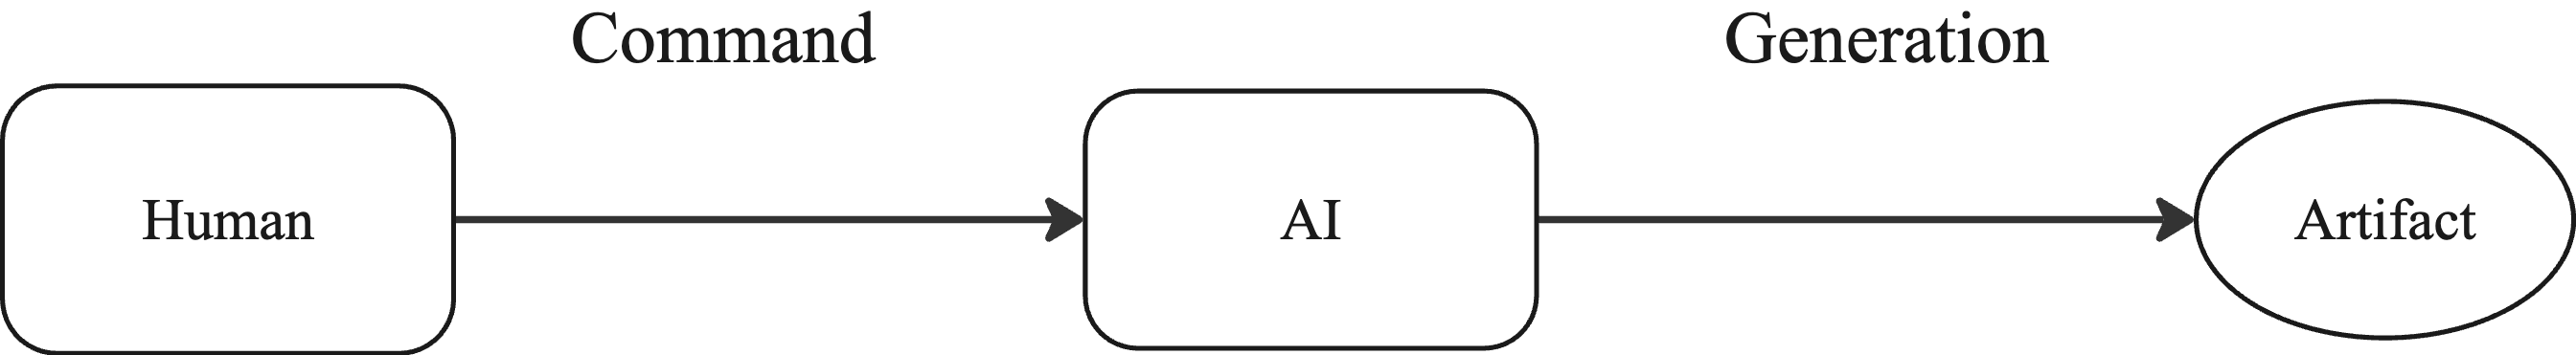
\includegraphics[width=0.75\linewidth]{unidirectional.png}
    \caption{Example of an unidirectional interaction with a generative AI system}
    \label{fig:unidirectional}
\end{figure}

However, as computers increasingly exhibit creative potential, the conventional command--execute paradigm becomes insufficient for fostering collaborative relationships. Instead, effective \emph{co-creative} engagement calls for \emph{dynamic back-and-forth conversations}, wherein both human and AI agents participate in iterative cycles of mutual understanding and influence. This is what I refer to by dialogic interaction. Importantly, in a dialogic process, participants can communicate \emph{both through} the creation itself and \emph{about} the creation (see Figure \ref{fig:dialogicthroughandabout}), thereby enabling deeper collaboration. As such, conversation may be a part of it, but not the exclusive component. 

\begin{figure}
    \centering
    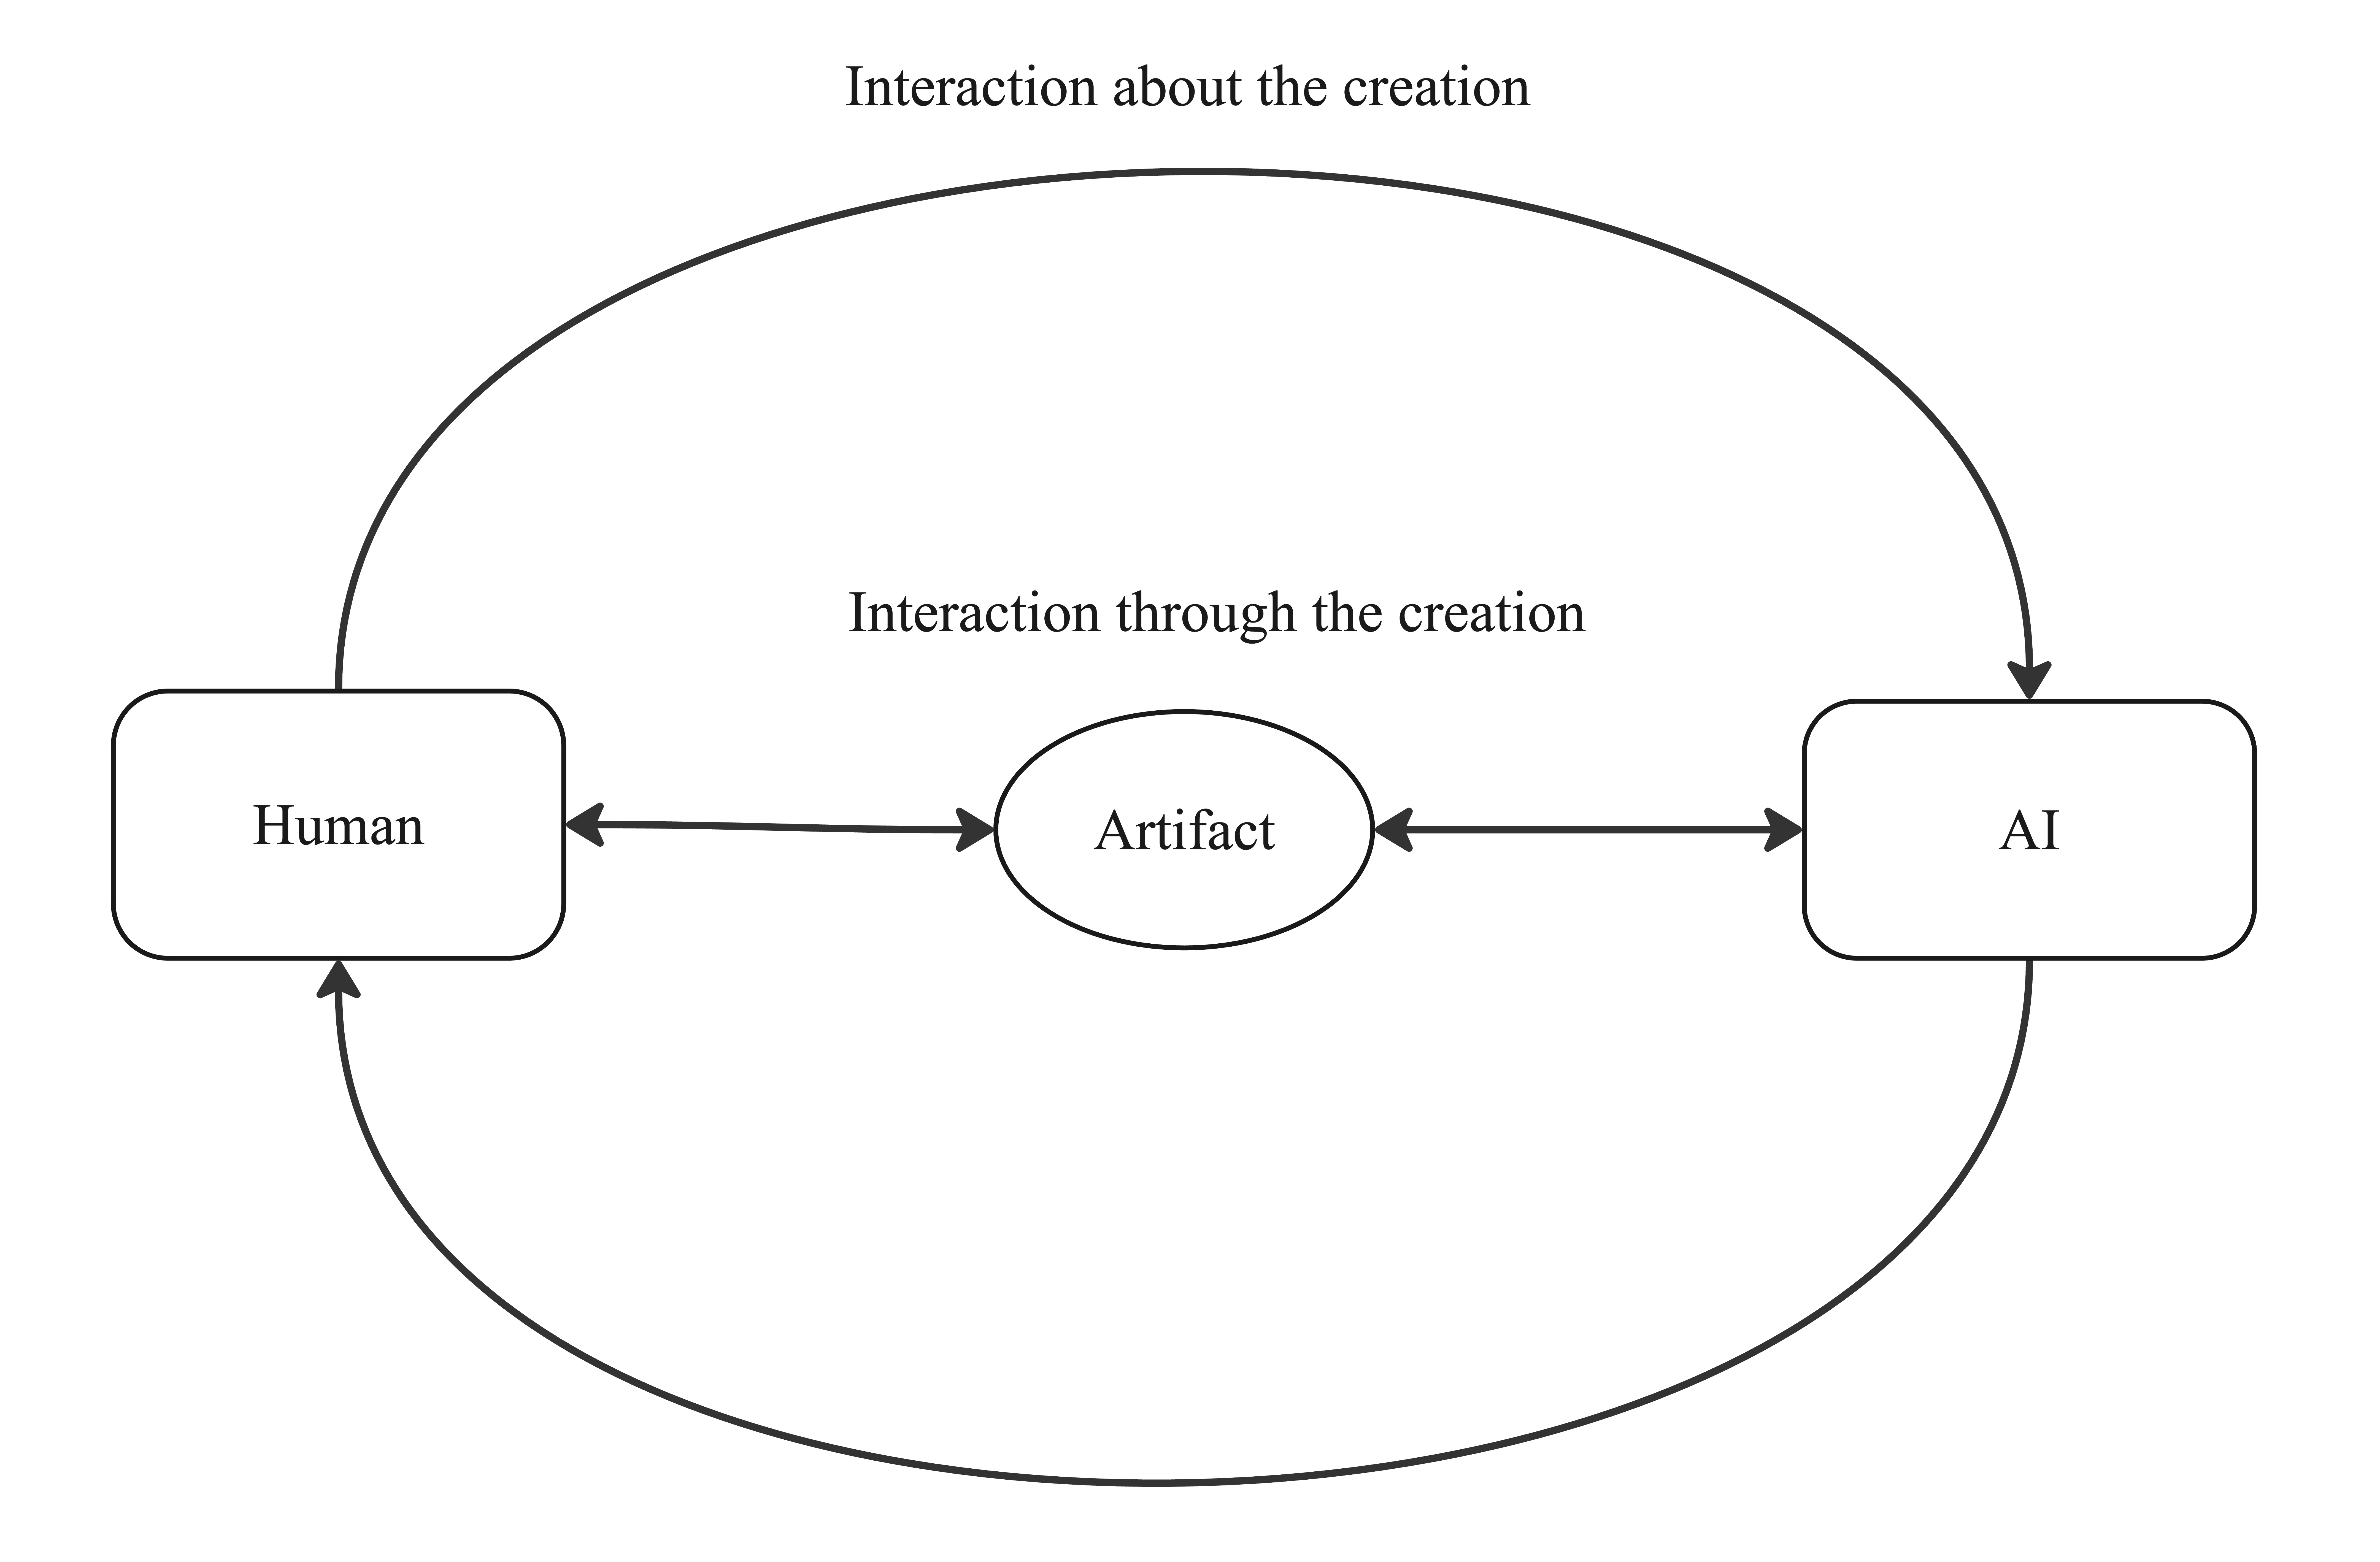
\includegraphics[width=0.75\linewidth]{dialogicthroughandabout.jpg}
    \caption{Diagram showing a dialogic interaction between a human and generative AI system interacting through and about the creation}
    \label{fig:dialogicthroughandabout}
\end{figure}

Dialogue has long been discussed in fields such as Human--Computer Interaction (HCI) and creative practice as a means to model interactions with computers and creative tools. Despite this, it remains underformalized as an interaction design concept in HCI. My research, conducted as part of an Australian Research Council (ARC)-funded project exploring Dialogic Creative AI, builds on initial work by Grace and Bown to address this gap.

In light of the emergence of chat-based interfaces as the predominant mode of interaction with language models, it might seem self-evident that dialogic interaction can enhance co-creativity. However, my characterization of dialogue extends beyond bidirectional text exchanges. By drawing on philosophical, educational, and interdisciplinary dialogue literature, I develop a more comprehensive construct of \emph{dialogic interaction}---an original contribution to HCI---comprising six key elements:

\begin{itemize}
    \item Bidirectional communication
    \item Shared collaborative space
    \item Iteration
    \item Mutual Influence
    \item Mutual Understanding
    \item Context-awareness
\end{itemize}

These elements are discussed in detail in Chapter~3. Notably, while bidirectional textual exchanges (as exemplified by popular chat interfaces) constitute one component, my proposal predates the widespread adoption of chat-based interactions, including the late 2022 launch of ChatGPT. The public success of such interfaces underscores the value of \emph{one} aspect of dialogic interaction---namely, real-time two-way communication---yet many other elements remain to be explored. Throughout this thesis, I examine how these additional elements can further support effective human--AI co-creativity.

Against this backdrop, I formulated one overarching research question and three sub-questions to guide this inquiry:

\begin{quote}
\textbf{Core Research Question:}\\
\emph{How can we design generative AI systems that act as effective co-creators, maintaining human agency while effectively leveraging the creative potential of this technology?}
\end{quote}

\begin{quote}
\textbf{Sub-Questions:}
\begin{enumerate}
    \item \textbf{R1:} \emph{How does interaction design influence the role that humans and AI play in creative production?}
    \item \textbf{R2:} \emph{What is the potential of modelling dialogue in interaction design to enable effective human–AI co-creativity?}
    \item \textbf{R3:} \emph{Which interaction design principles can guide the development of effective co-creative systems?}
\end{enumerate}
\end{quote>

\subsubsection{Methodology}
To address my research questions, I adopt a mixed-methodology approach integrating qualitative and quantitative research methods across two strands: interaction design research and creative-led practice.

I focus specifically on human–AI co-creativity within three creative domains: writing, image generation, and interactive new media music installations. On one hand, I develop prototypes that are tested with users to evaluate the potential of dialogic interaction in enabling human–AI co-creativity. On the other hand, I engage in a creative practice-led approach by developing interactive artworks and collaborating with professional creatives in the completion of projects leveraging generative AI, which I then analyse as case studies. Through this analysis, I discuss both the potential and the limitations of these systems to be co-creative in real-world scenarios, with particular emphasis on dialogic interaction as a lens of analysis.

A diagram illustrating the approach and methodology is shown in \ref{fig:approach_figure}.

\begin{figure}[hbt!]
    \centering
    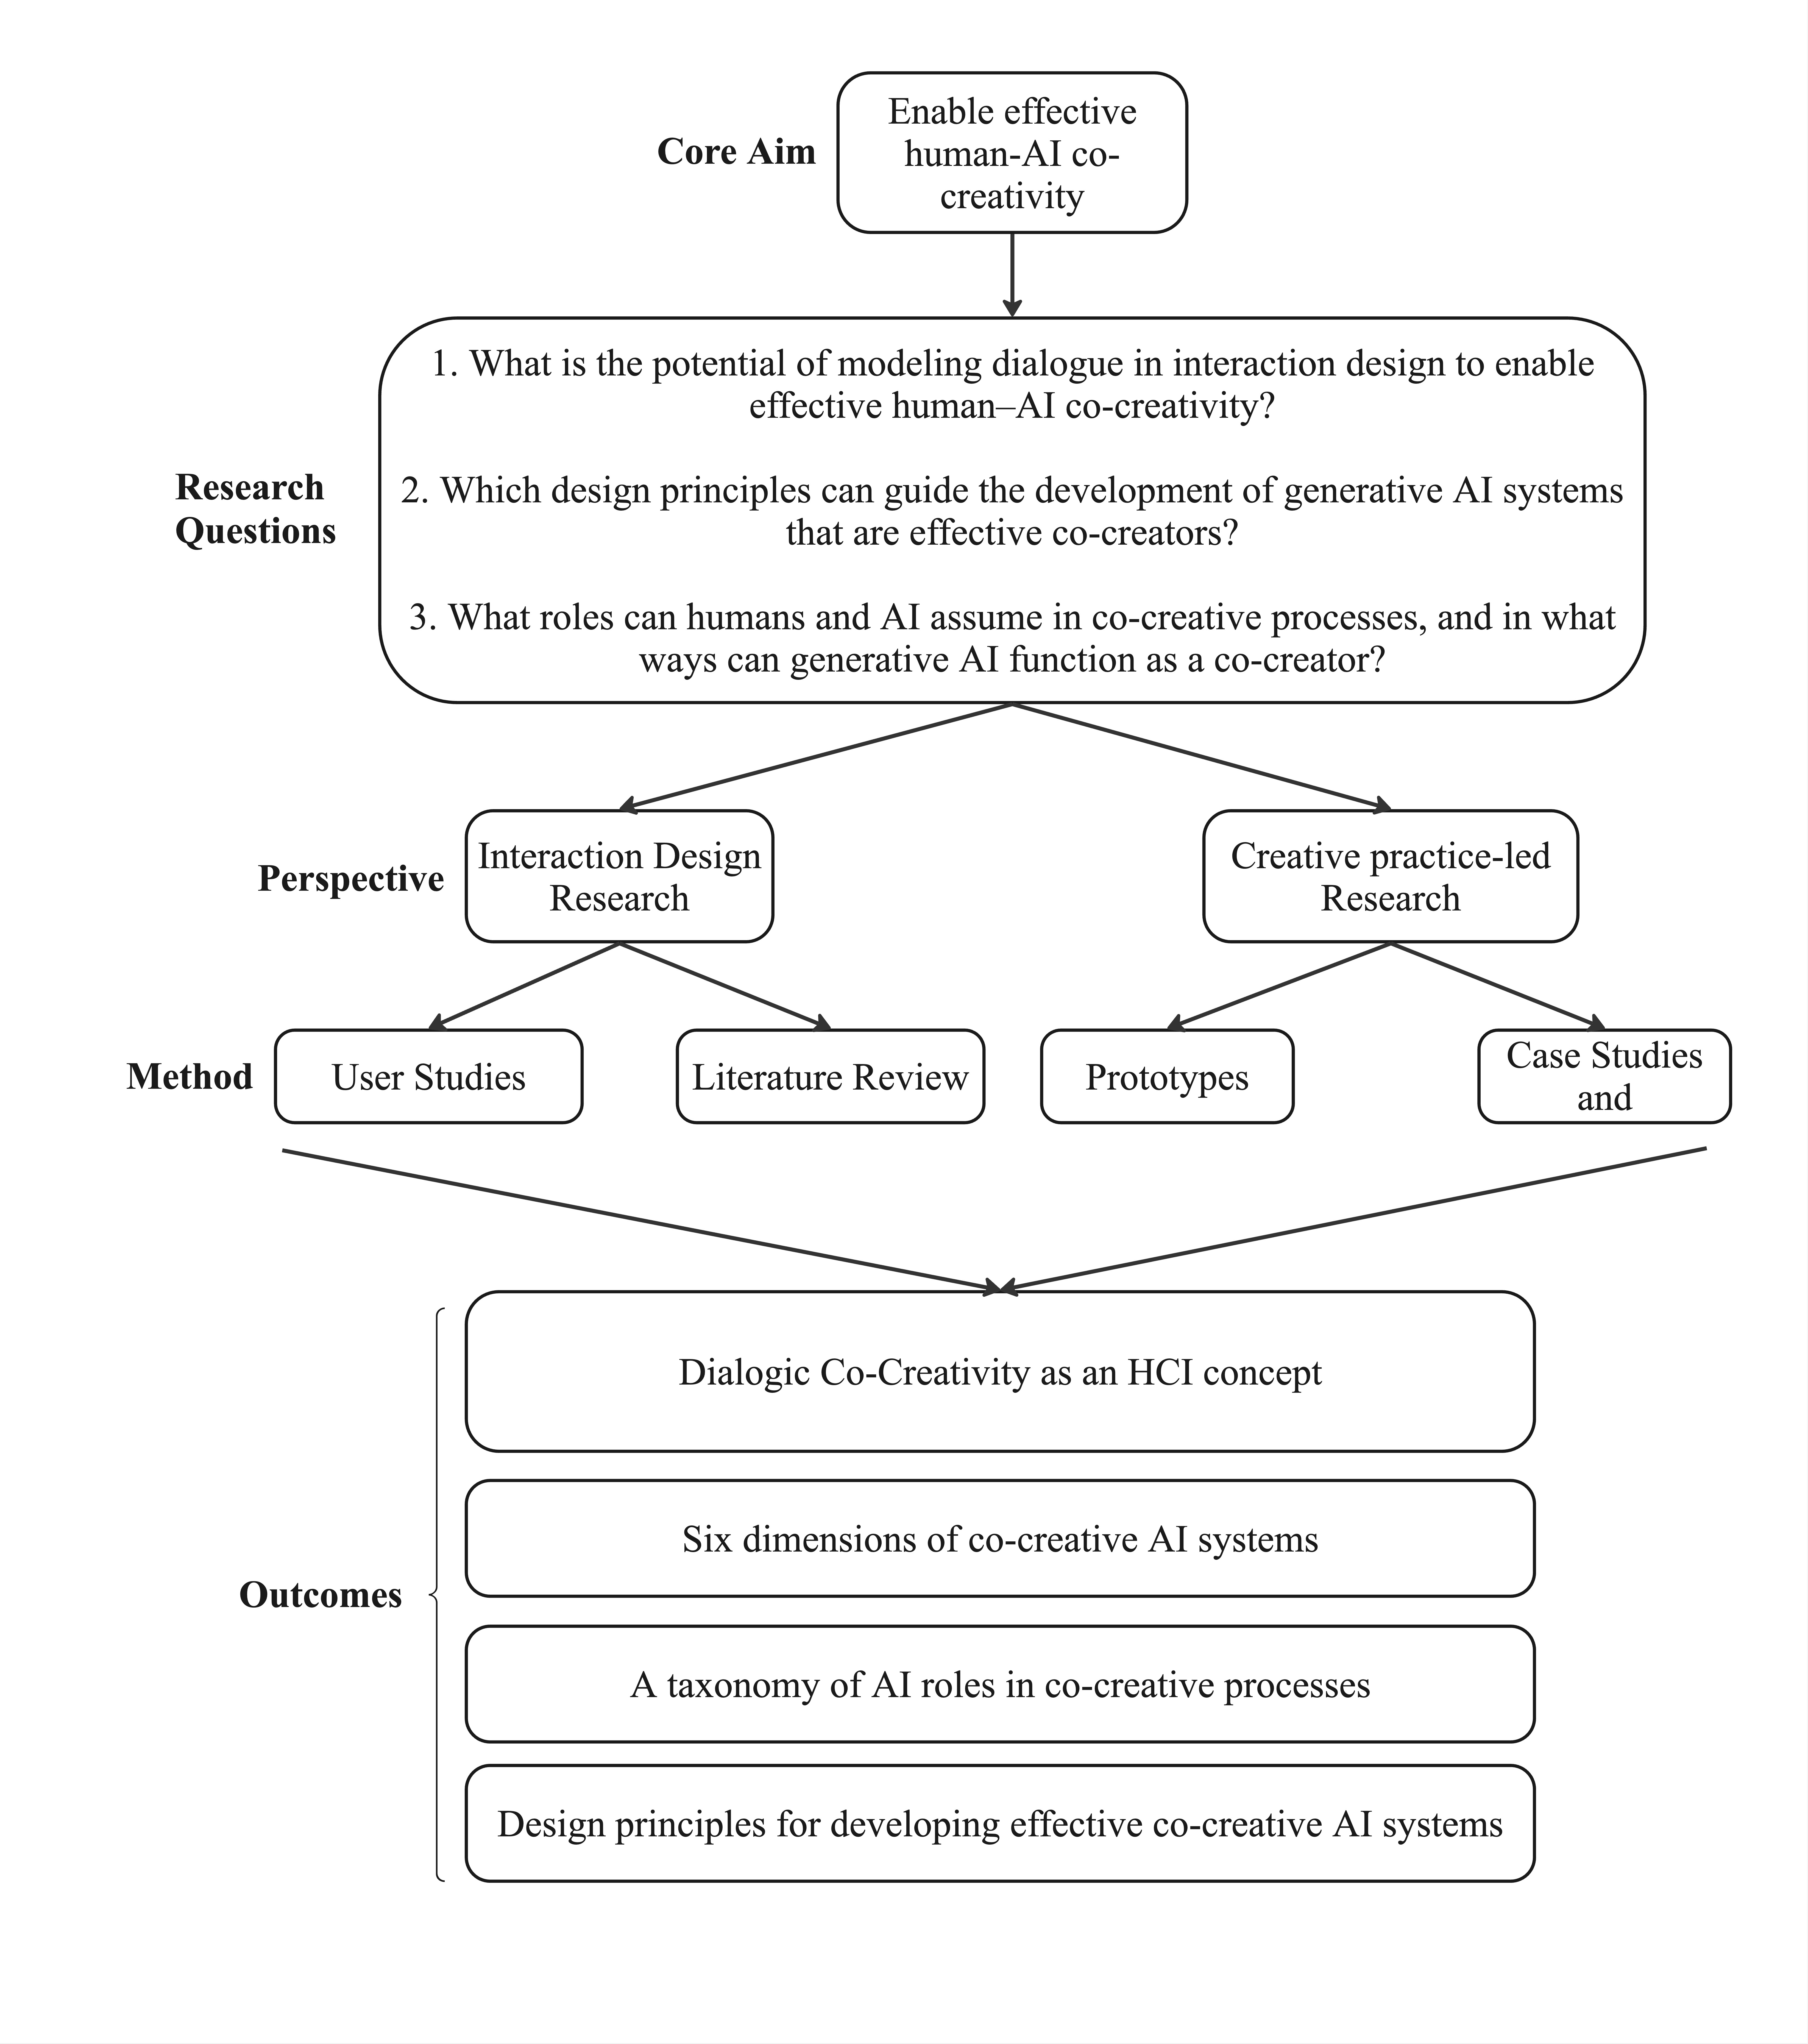
\includegraphics[width=1\linewidth]{Intro - Frame 1 (2).jpg}
    \caption{Diagram illustrating the approach followed to address the core research aim}
    \label{fig:approach_figure}
\end{figure}

\clearpage

\section*{Thesis Structure}

This thesis is structured chronologically but not strictly so, as I also prioritised grouping studies by creative practice: writing, image generation, and interactive sonic art installations. As such, the three primary study chapters—Chapters 4, 5, and 6—are organised accordingly. The preceding chapters establish the theoretical foundations that underpin the thesis, while the final chapter (Chapter 7) integrates the findings and conclusions.

\subsection*{Chapter 2: Literature Review}

Chapter 2 provides a literature review, contextualising the research within the broader field. It begins with an overview of state-of-the-art developments and recent progress in generative AI, establishing the technological landscape and its fundamental capabilities and limitations. The chapter then reviews key literature in computational creativity and human-AI co-creativity, followed by a discussion of dialogue as a relevant concept in interaction design. Although some aspects of dialogue are covered here, a more detailed exploration is presented in a dedicated chapter. The final section of Chapter 2 examines related approaches that apply dialogue as an interaction design concept in human-computer co-creativity.

\subsection*{Chapter 3: Conceptual Foundations of Dialogic Co-creativity}

Chapter 3 lays the conceptual foundations for dialogic co-creativity as an interaction design framework within Human-Computer Interaction (HCI). This chapter consists of two parts. 

\subsubsection{Preliminary Framework for Dialogic Co-creativity: } The first part includes a paper presented at the CHI Workshop on Generative AI (2022), where I introduced a preliminary framework for dialogic interaction. This early work explored bidirectional communication with language models in creative contexts. At the time, chat-based interfaces were not the dominant interaction paradigm for language models; most interactions were based on autocomplete or linear instructions. Through prompt engineering, we investigated the feasibility of engaging with AI in conversational creative dialogue, interacting both through and about the creation. This introduced distinction—interaction *through* versus *about*—became a central theme of dialogic interaction throughout the thesis.

\subsubsection{Six elements of dialogic co-creativity:} The second part of Chapter 3 was developed towards the later stages of my research and presents a more formalised definition of dialogic interaction. This definition is articulated through six key elements:

\begin{enumerate}[label=\arabic*.]
    \item Bidirectional Communication
    \item Shared Space
    \item Iteration
    \item Mutual Influence
    \item Mutual Understanding
    \item Context-Awareness
\end{enumerate}

These elements serve as the foundation for analysing and designing co-creative systems that facilitate human-AI collaboration.

\subsection*{Chapter 4: Co-Creative Writing}

Chapter 4 explores co-creative writing through two case studies. 

\subsubsection{Narrative Device: } The first part examines \textbf{Narrative Device}, an early prototype developed in late 2021 and early 2022. This prototype allowed users to input two distinct concepts, which a language model then combined to generate short stories, drawing on Boden’s concept of combinatorial creativity. The system, which was publicly released and gained viral popularity, facilitated the creation of over two million stories by more than a hundred-thousand users. For many users, this was their first experience of co-creating with a highly capable AI system.

On one hand, Narrative Device required users to engage in creative ideation by choosing concepts that, when combined, would produce an interesting or humorous story. On the other hand, the creative potential of AI was drawn to integrate these elements coherently and surprisingly (following the constraint of both novelty or surprise and value). While the system was positively received and users expressed satisfaction with it, a fundamental challenge was that, it did not allow users to iterate or refine the generated stories. This lack of \textbf{iteration} is an element of dialogic interaction and a common limitation expressed by users of this and other systems. This limitation stemmed in part from the fact that the underlying model (InstructGPT) was designed primarily for instruction-following rather than conversational interaction.

Following the release of ChatGPT in late 2022, chat-based conversational interfaces became the dominant paradigm for AI-assisted writing. While this bidirectional communication mode enabled greater iterative collaboration, I observed that it was limited for co-creativity as it primarily facilitated interaction *about* the creation rather than *through* it. This shift often leads users to assume an outsourcer role, delegating writing tasks to the AI rather than engaging in co-creation. Research suggests that this tendency can negatively impact users’ creative agency, self-efficacy, and involvement, and that interface design can mitigate this effect by encouraging deeper engagement \cite{Kantosalo2016-hg, McGuire2024-im}.

\subsubsection{From Instructors to Co-Authors: Mitigating Overreliance on AI Through Collaborative Writing Interfaces (manuscript submitted to ICCC 2025)} To address these challenges, I developed a second prototype in two iterations across 2023 and 2024. These prototypes introduced a collaborative text editor, enabling both human and AI to read and modify the text, alongside a chat window for discussing writing goals and making requests. This design allowed users to interact with the AI both through and *about* the creative process. 

Two user studies were conducted to evaluate this prototype. Unlike \textit{Narrative Device}, these studies were controlled and not publicly released. Although the participant sample was limited, they highlighted the potential of this interface to enhance human involvement. In the chat-only condition, users were more likely to agree that the AI had done most of the work. In contrast, in the shared editor condition, users reported contributing more of their own writing and assuming more active roles as co-creators. The development of these prototypes anticipated industry trends: a few months after these prototypes were developed, commercial AI tools integrated similar collaborative interfaces. For instance, Anthropic’s Claude introduced Artifacts in August 2024, followed by OpenAI’s Canvas for ChatGPT in October 2024. These developments reinforce the importance of integrating collaborative workspaces with chat-based interactions for human-AI co-creativity.

\subsection{Chapter 5: Interactive Sonic Art Installations}

Chapter 5 is comprised of two papers, each describing an interactive sonic art installations developed over two years. These installations primarily explored the dialogic co-creativity element of context-awareness, such that generative AI can act as a co-creator within a context, taking actions that affect that context, while maintaining human compositional and creative intent. 

Both of these installations were data sonificiation installations where an LLM was used a semantic interpretive bridge between data and and a generative soundscape. 

\subsubsection{Using GPT-3 to Achieve Semantically Relevant Data Sonificiation for an Art Installation: } This paper, presented at EvoMusArt 2023 in Brno Czech Republic, describes an installation commissioned by the Australian National University School of Cybernetics and developed in collaboration with Uncanny Valley, was presented at the Cybernetic Serendipity festival. The goal was to transform both the built and natural environment surrounding the festival into a dynamic soundscape. Live data streams—including global CO$_2$ levels, national economic indicators, and local weather conditions—were interpreted by a language model, which generated succinct textual descriptions. These descriptions were then converted into word embeddings and mapped onto a latent space of musical descriptors, creating a continuously evolving soundscape.

\subsubsection{Interpretative Data Sonification: Using LLMs to Interpret Data and Generate Continuous Soundscapes at the Sydney Opera House} This paper, presented at the Sound and Music Conference 2024 in Porto, Portugal describes a second installation, commissioned for the Sydney Opera House’s 50th anniversary, built upon this approach but with greater AI agency. Instead of merely interpreting data, the AI actively controlled aspects of the music generation process based on real-time environmental inputs, including building energy use, water consumption, and ongoing performances.

Through this installations, we showed the potential for large language models to understand and interpret complex structured and unstructured data, and then use those interpretations to drive a generative artwork. As such, becoming context-aware co-creators, that can act within it and take actions that affect it key element in dialogic interaction. 

However, both installations revealed challenges for this context to be acted upon effectively, particularly context window limitations and maintaining historical coherence over extended durations. The AI tended to fixate on certain patterns, limiting the generative scope. However, these works highlighted the potential of AI-mediated semantic interpretation in real-time reactive sound art, moving beyond direct data-to-sound mappings.

\subsection*{Chapter 6: Generative AI in Design and Media}

Chapter 6 presents two case studies exploring the co-creative potential of generative image and language models in visual domains, particularly focusing on the \textbf{iterative element of dialogic co-creativity}. 

\subsubsection*{AI-Assisted Interior and Furniture Design}

This project, in collaboration with Studio Snoop in Sydney, explored the use of AI in furniture and interior design. It resulted in an AI co-creator named *Tilly*, integrating a language model and a text-to-image model. The system was used to ideate and generate designs aligned with sustainability, natural materials, and human well-being. The project culminated in an installations at Milan Design Week where posters of the designs where shown. Attendees provided daily feedback to Tilly, an AI, which then informed design iterations by a team in Sydney.  This process culminated in a final design presentation at the end of the week.  Later that year, these designs were physically produced by artisans and studios worldwide and showcased at the London Design Festival. The project explored how generative AI can act as a co-creator, facilitating iterative, distributed creativity across time and space.

\subsubsection*{AI-Generated Portraits for the Australian Financial Review (AFR)}

This study, conducted with AFR Magazine, and presented at the 2024 International Conference on Computational Creativity (ICCC) in Jönköping, Sweden explored AI-generated portraits for their annual "Most Powerful People in Australia" feature. The goal was to create concept-driven images that reflected each subject’s personality and role. For example, the head of the Federal Reserve piloting a balloon as a metaphor for their control of inflation. The iterative collaboration between the AI system and human designers revealed challenges in controlling generative outputs and maintaining visual consistency. The publication of these AI-generated portraits sparked public debate, highlighting ongoing concerns about AI's role in creative industries.

\subsection*{Chapter 7: Conclusion}

The final chapter synthesises the findings from previous chapters and presents four key contributions:

\begin{enumerate}[label=\arabic*.]
    \item The potential of dialogic interaction to enable effective human-AI co-creativity.
    \item A novel characterization of six dimensions of co-creativity for designing generative AI systems.
    \item A taxonomy of AI roles in co-creative processes.
    \item A set of design principles for developing effective co-creative AI systems.
\end{enumerate}

These contributions provide insights for both researchers and practitioners in designing AI systems that foster meaningful human-AI collaboration.
    \chapter[Literature Review]{Literature Review}

The aim of this thesis is to investigate the development of effective human-AI co-creativity from the perspective of interaction design. This aim spans a multidisciplinary literature, including the psychology of human creativity, computational creativity, human-computer interaction and emerging empirical and theoretical literature on human-AI co-creativity. 

The present chapter covers this multidisciplinary literature with a primary focus on interaction design. More specifically, I use the following core question and three sub-questions as a navigational lens:

\begin{quote}
\textbf{Core Research Question:}\\
\emph{How can we design generative AI systems that act as effective co-creators, maintaining human agency while effectively leveraging the creative potential of this technology?}
\end{quote}

\begin{quote}
\textbf{Sub-Questions:}
\begin{enumerate}
    \item \textbf{R1:} \emph{How does interaction design influence the role that humans and AI play in creative production?}
    \item \textbf{R2:} \emph{What is the potential of modelling dialogue in interaction design to enable effective human–AI co-creativity?}
    \item \textbf{R3:} \emph{Which interaction design principles can guide the development of effective co-creative systems?}
\end{enumerate}
\end{quote}

This literature review is structured in two main parts. The first part establishes foundational concepts by defining human-AI co-creativity and creativity more broadly, before identifying the current gap in design principles for co-creative systems. The second part then addresses the three research questions in reverse order: beginning with design principles (R3), then exploring the potential for dialogic interaction (R2), and concluding with an analysis of roles in human-AI co-creative processes (R1). 

\section{Defining human-AI co-creativity}

In the previous chapter, I provided the working definition of co-creativity as:

\begin{quote}
\emph{A type of human-AI interaction involving creative contributions from both human and AI and where the outputs cannot be uniquely or primarily attributed to the creative behaviour of one of them.}
\end{quote}

This definition is informed by the work of \cite{Candy2002-ra} discussing human-human co-creativity as a closely woven interaction that produces outputs from symbiotic combination of actions, and from the work of Davis (2013), \cite{Davis2013-jy} who described human-computer co-creativity as an interaction where the computer is not just a rigid executor of commands but adapts dynamically, drawing on computational creativity algorithms to respond to the user. Since then, a growing literature frames human-AI co-creativity as a type of interaction that ultimately augments human creativity and can mitigate risks associated with the automation of creative work \cite{Yannakakis2014-zs, Kantosalo2020-zf, Rezwana2022-gg, Moruzzi2024-cq, Haase2024-yp, Lin2023-zq, Karimi2018-wi}. It has also been proposed as a type of interaction that can not only help humans be more creative, but computational creative algorithms be more creative \cite{Liapis2016-zt}. That is: the ultimate aim is that together, human and machine can produce more creative outputs than either could produce alone and where both are exercising creative behaviour. 

\section{Defining Creativity}

My discussion of human-AI co-creativity will benefit from establishing a working definition for creativity. However, defining creativity is not an easy task. Part of the complexity stems from the fact that when describing something as creative, we may be referring to at least one of four things: it can refer to a person (e.g., "Frida Kahlo was very creative"), a process (e.g., "my creative process"), a product (e.g., "this story is very creative"), or an environment (e.g., "a very creative city"). These four components were initially conceptualised by Rhodes \cite{Rhodes1961-od} as the 4Ps of creativity: Person, Process, Product, and Press, and today remain an influential framing for discussing creativity, and more recently, co-creativity \cite{Kantosalo2019-pz}. 

Notwithstanding the acknowledged complexity of such a wide-encompassing term, the scientific literature has largely converged to using The Standard Definition when discussing and measuring creativity. The Standard Definition provides a double constraint as a bar for creativity: something is creative if it's both considered \textbf{novel (or surprising)} and \textbf{valuable (or appropriate)} \cite{Amabile1983-lj, Sternberg1998-oz, Runco2012-mk, Boden2003-hk}. It follows from this definition that this double constraint could be applied to a Product, a Person, a Process or an Environment (Press). For example, a creative painting (Product) may be one that is both different (novel) to existing works and beautiful (if that is the value being applied). Similarly, a Person is one that produces such a work, a creative Process is one that this person employs and a creative environment in which this is produced and shared (Press). As such, a human-AI co-creative system is one that produces, as a result of meaningful contributions from human and machine, a novel and valuable output. 

A natural question emerges: can a computer by itself produce creative work, and is the Standard Definition sufficient to capture the richness of what is involved in creativity? Indeed, this has been a point of contention since the birth of computers, and it has been a more vivid debate since the inception of the field of artificial intelligence. Turing argued for the capacity of machines to produce novel things through their ability to surprise the human user when addressing the Lovelace Objection \cite{Turing1950-aq}. The Dartmouth Summer Research Project on Artificial Intelligence, where the term Artificial Intelligence was first used and which many consider as the genesis of AI research \cite{McCarthy1955-ls}, established “Randomness and Creativity” as one of the seven areas of research for the field. 

Simon and Newell, whose Logic Theorist is often cited as the first AI program \cite{Russell2016-oe}, argued that creative thinking is an extension of ordinary problem‑solving, navigating vast problem spaces through trial and error to find solutions that are both \textit{novel} and \textit{useful}\cite{Simon1967-nr}. Boden framed creativity, both human and computational, as movement within and transformation of “conceptual spaces” through combination, exploration, and transformation \cite{Boden2003-hk}. A human might move through conceptual spaces in their head based on ideas they have been exposed to. A computer may move through these spaces based on data it has been trained on, or in the possible application of rules. This framing of creativity as searching through conceptual spaces was formalised by Wiggins in his Creative Systems Framework, providing a mathematical account creativity as search within conceptual spaces  \cite{Wiggins2006-zd}.

In more recent times, Computational Creativity has grown as a robust field on its own, developing across a literature that seeks to formalise what it means for a computer to be creative, how this can be implemented in computer programs, how creative behaviour of computers can be measured \cite{Ritchie2007-jy, Colton2008-fh, Colton2011-uy, Maher2012-oj, Jordanous2012-kw}, as well as rich creative practices that employ computers both as tools, and as autonomous and collaborative creative agents \cite{Cohen1995-wt, Colton2015-qr, Perez-y-Perez1999-ma, Cope1992-pq, Reichardt1968-eo}. This interdisciplinary nature of computational creativity has been captured in the working definition for computational creativity provided by Colton and Wiggins \cite{Colton2021-bt}.

\begin{quote}
The philosophy, science and engineering of computational systems which, by taking on particular responsibilities, exhibit behaviours that unbiased observers would deem to be creative.
\end{quote}

While computational creativity was considered historically as a final frontier of artificial intelligence research \cite{Colton2021-bt}, today, empirical evidence shows that computers are increasingly showing creative behaviour according to the standard measures we use to measure human creativity. For example, computers are now able to perform at a similar or higher levels than humans in the Alternative Uses Test, which measures the ability of a person to produce a high number of novel and valuable uses for a given object \cite{Hubert2024-kv, Guzik2023-cl}. Computers have shown to be able to produce a wide variety of artefacts that human raters consider creative, and sometimes, prefer to those produced by humans, especially when they do not know it was produced by generative AI \cite{Alexander2024-pz, Wu2025-or, Kobis2021-bb}. 

This may be sufficient to acknowledge that computers are capable of producing creative outputs. However, some creativity researchers have rebuked this claim by arguing that creativity requires things other than the ability to produce novel and valuable outputs. Runco, one of the original contributors to the Standard Definition, acknowledged that “AI can be original, and its output is often useful,” but that \emph{authenticity} and \emph{intentionality} must also be present \cite{Runco2025-bu}, qualities he deems computational agents incapable of possessing. While this argument may appear as a case of merely moving the goalpost, a more benign reading may concede that Runco's argument is one of category. After all, he proposes that what we observe in computers should be better termed as \textit{artificial creativity}, and be distinguished from \textit{human creativity}. 

These arguments touch on a broader discussion on creativity, which seek to understand different forms that creativity may take across human and non-human systems. For example, a growing body of literature proposes creativity can exist in distributed complex systems such as societies and evolution. Under this view, natural selection can be considered as a creative process producing solutions to the problem of survival, even if this process is very different from that of human creativity \cite{Wagner2015-oj}. Bown proposes a distinction between \textit{adaptive creativity}, to refer to the kind that a human might engage in when trying to solve a problem with a clear defined goal and value criteria, and \textit{generative creativity}, which may refer to the kind that a non-human self-organising complex system may produce \cite{Bown2012-gg}. 

This discussion similarly extends conceptions of creativity as something that exists beyond the individual. While often, particularly popular and media descriptions of creativity view it as emanating from the genius of sole individuals, broader perceptions of creativity see it as a result of interaction between human and non-human agents. People create within contexts and environments, embedded within cultural norms. They use tools, language and musical scales created by other people. All of these elements exercise varied degrees of influence on the person, their process and their output. As such, some authors argue that creativity may be better understood as acting within \textit{networks of agency}, where agency is shared between multiple parties, rather than emanating from a sole source \cite{Brown2016-tc, Malafouris2008-xn}. 

In the case of human-machine co-creativity, the agencies between human and tool are blended and more equally shared, to a degree such that the term "tool" may not be adequate anymore \cite{Lawton2023-tb}. 

\section{The gap: a lack of principles for human-AI co-creativity}

I have established, albeit broadly, how humans and machines can be creative, and laid the ground to understand how they can be creative together. In the next sections, I will focus particularly on this issue from an interaction design lens. That is: how can we design AI systems that effectively co-create with users. 

While in other fields there are established principles and heuristics for designing effective human-computer interaction and tools that support creativity \cite{Nielsen1994-df, Amershi2019-vy, Shneiderman2020-je, Wright2020-nt, Bengler2012-jf, Resnick2005-fs}, the field of human-AI co-creativity lacks specific guidelines that capture the nuance and complexity of humans and machines blending creative agencies successfully. 

Historically, new advances in computational capabilities have required new interaction design principles. The transition from mainframes to personal computers led to the development of Apple's the Human Interface Guidelines in 1987, which have been updated with each new computational paradigm such as the internet and mobile computing. Similarly, the transition to generative AI as an underlying computational layer requires new guidelines for interacting with it. Already, the use of old interaction paradigms to interact with generative AI has led to notable limitations: what Koomen \cite{Koomen2025-eu} has termed the AI Horseless Carriage problem. Koomen draws a parallel between interacting with generative AI using old interaction paradigms with the phenomenon of early motor cars being designed simply as horseless carriages, rather than as new types of vehicles on their own. 

This does not mean, however, that existing work is not relevant: as we will see in the following sections, many of the shortcomings reported in human-AI co-creativity studies can be addressed with principles present in the existing literature. Moreover, any effort seeking to provide guidelines, principles and heuristics for human-AI co-creativity would greatly benefit from starting from this existing time tested-work on human-computer interaction. 

However, generative AI poses new specific challenges that often are at odds with previous design heuristics. An example is what Weisz et al. \cite{Weisz2024-io} terms \textit{generative variability}, where the same input may produce different results each time. In many cases, this is a feature, not a bug, of generative systems. However, it may stands at odds with design principles such as Nielsen's consistency \cite{Nielsen1994-df} of input-outputs. On the user side, advanced capabilities of new generation AI systems are beginning to lead to more over-reliance on these tools, which ultimately may hinder performance in the short term and lead to skill loss in the longer term \cite{Buschek2021-ks, Dell-Acqua2022-dy, Gerlich2025-as}. Buschek et al. \cite{Buschek2021-ks} described nine potential pitfalls when designing co-creative generative AI, including invisible boundaries of AI capabilities, lack of expressive interaction control, a false sense of proficiency, overwriting user work, agony of choice, unclear ownership of the work, and privacy risks related to training on user data. Many of these are not adequately addressed with existing principles and heuristics.

Consequently, some authors have proposed principles for interacting with generative AI. For example, \cite{Amershi2019-wu} proposed a set of Guidelines for Human-AI Interaction and Weisz et al \cite{Weisz2024-io} proposed a series of Design Principles for Generative AI systems. However, these systems focus on generative AI systems as a whole, and do not specifically deal with the intricacies of co-creativity. For example, one of Weisz et al's principles simply states: "Design for Co-Creativity", however, no specific directives are provided for enabling such co-creativity. Indeed, designing for co-creativity is a complex challenge in itself \cite{Buschek2021-ks}. 

\subsection{Frameworks and Taxonomies}

While there are no design principles for human-AI co-creativity, the literature has produced extensive work classifying and describing co-creative AI systems, in the form of taxonomies and frameworks. As early as 2019, Guzdial and Riedl provided an Interaction Framework for Studying Co-Creative AI \cite{Guzdial2019-gr} and Kantosalo's PhD dissertation provides one of the most detailed accounts for describing, evaluating and designing human-AI co-creativity in the context of poetry writing \cite{Kantosalo2019-pz}. 

More recently, Rezwana \cite{Rezwana2022-gg} proposed the Co-Creative Framework for Interaction Design (COFI), which provides an extensive account of the different possibilities for designing co-creative AI systems. Moruzzi and Margarido proposed a user-centered framework for human-AI co-creativity, which similarly describes in detail different dimensions to be considered when designing co-creative systems, which they propose should be controlled and personalised by the user \cite{Moruzzi2024-cq}. Haase and Pokutta developed a classification for different levels of creative collaboration between humans and AI, from simple task level automation to what they term full co-creation \cite{Haase2024-yp}. 

Lastly, the literature is rapidly producing empirical studies evaluating different ways in which interaction design affects aspects of human-AI co-creativity. As such, there is a ripe opportunity to critically analyse these findings and produce a theoretically grounded and empirically informed set of design principles for human-AI co-creativity. The intention of this review is to collate these findings and leverage the frameworks described above to interpret them, such that by the end of this thesis, a clearer picture of the interaction design principles that can contribute to effective human-AI co-creativity emerges. 

\subsection{The Challenge of Effective Co-Creativity}

A first challenge faced when seeking to understand what factors contribute to effective co-creativity arises in measurement. What defines effective co-creativity, in the first place? Currently, the metrics used to measure this can be broadly classified in two types. First, self-reported metrics that gather subjective user experiences, such as user satisfaction, enjoyment, creative self-efficacy, frustration and other similar evaluations. Second, observed metrics that assess task completion time, quality, creativity, and quantity of outputs, often rated by crowdsourced evaluators or experts \cite{Kim2021-fh, Kantosalo2019-pz, Rezwana2022-ui, Rezwana2023-gj, Lawton2023-tb}. Thus, effectiveness evaluations typically combine both process-oriented and outcome-oriented perspectives, encompassing both subjective and objective data.

It is worth noting that process-oriented evaluations do not always align with product-oriented evaluations. For example, a particular interface design may lead to higher third person ratings of creative writing outputs, but lower satisfaction and enjoyment of the user with the process and interaction \cite{Lee2022-rj}. 

Moreover, there remains a lack of standardised metrics or benchmarks for evaluating co-creative systems, reflecting broader methodological challenges already identified within computational creativity research \cite{Jordanous2012-kw}. Some researchers have sought to remedy this by proposing comprehensive, robust metrics and measurement frameworks across process and product \cite{Kantosalo2019-pz, Davis2016-te, Lawton2023-gd, Lee2022-rj}. 

However, my analysis of the literature revealed many of these standardised measurements are rarely used, and measurement is commonly idiosyncratic. This often leads to contradictory findings and lends itself to overly broad claims within the literature. For example, generalised assertions such as "AI enhances creativity" or "AI diminishes creativity" are common but problematic, and they are akin to claiming broadly that computers or the internet impact creativity positively or negatively. The specific nature of the interaction and targeted outcomes must be clarified to yield meaningful insights.

One illustrative example is a study titled "An empirical investigation of the impact of ChatGPT on creativity," published in Nature Human Behaviour \cite{Lee2024-vz}. The study reported that using ChatGPT during ideation tasks enhanced creative outputs compared to individual human ideation or using web search. Notably, the paper claimed human modification did not further improve the creativity of AI-generated ideas, and the authors suggested in some cases computers may act more effectively as autonomous creators. However, critical details regarding how participants interacted with ChatGPT were left unclear. On one hand, the paper states that humans only submitted one idea after selection. Arguably, this curation involves a form of modification and co-creative interaction in itself. Moreover, it is not clear how this selection was enabled. Did they use iterative ideation cycles, exploring different possibilities in a conversation, or did they simply select from a static drop-drown of options? Clarifying these interaction details is essential to make claims about the impact of human-AI interactions in creative outcomes.

Moreover, results may vary depending on the task, the expertise of the user and the stage of the creative process. For example, it has been found that one of the most common uses for generative AI is ideation and brainstorming \cite{Zao-Sanders2024-qo}. However, a study with professional writers found they regarded language models as less useful for ideation but more beneficial for feedback, translation, and rewriting tasks \cite{Chakrabarty2024-ov}.

When assessing the impact of human-AI interactions in creative contexts, it is also crucial to examine not only individual creativity but also creativity at a collective level. For example, Doshi and Hauser \cite{Doshi2023-dv} investigated the effects of using generative language models for ideation during short story writing. The study revealed that participants using AI generated more creative stories, as rated by external evaluators, compared to those who did not use AI, particularly benefiting less experienced writers. However, the study found that the stories generated with AI assistance, while rated as more creative than the non-AI assisted ones, were \textit{more similar to each other} when measured for semantic similarity, suggesting a collective homogenisation effect.

Indeed, concerns regarding such homogenisation and reduced originality has been found to be a key detractor for generative AI adoption in creative activities, with users commonly reporting concerns with the lack of originality, generic outputs, and clichéd styles \cite{Chakrabarty2024-ov, Chang2023-tv, Clark1998-yi, Ippolito2022-mf, Li2024-yh}.

So far, this section has outlined several key challenges in evaluating and designing for effective human-AI co-creativity. The following sections will examine how specific interaction design factors that can foster more effective co-creative outcomes across diverse metrics, tasks, and users. 

\section{Towards Design Principles for Human-AI Co-Creativity}

\subsection{Visibility of Creative Capabilities}

A critical factor influencing the effectiveness of human-AI interactions is users' understanding of the AI system: that is, what it can and cannot do.

A study by Dell’Acqua \cite{DellAcqua2023-og} involving consultants from a major firm undertaking complex, partly creative tasks, provides an illustrative example. Results indicated improved performance and efficiency when using an LLM for tasks within its known strengths, yet decreased performance when tasks exceeded where the capabilities of the model are less reliable, such as factual accuracy and mathematical reasoning. The authors describe this phenomenon using the concept of the "jagged technological frontier": inside the frontier, AI usage typically benefits performance; outside, it often detracts from performance. However, this frontier is usually unclear: this is what \cite{Buschek2021-ks} described as invisible boundaries, with model creators and users alike frequently uncertain of the system’s precise capabilities.

However, training and onboarding that educate users of AI's capabilities can be effective to maintain involvement and improved outcomes. For example, recent research has reported that increased reliance on language models has been associated with reduced critical thinking skills due to cognitive offloading and over-reliance \cite{Gerlich2025-as, Lee2025-dw}. However, a study by Essel et al \cite{Essel2024-qc} actually found improved critical thinking among students using LLMs after they received training about the model's appropriate use as a critical thinking tool.

These contrasting outcomes highlight that many negative effects associated with AI use stem from users’ overreliance on systems, driven by automation bias and inaccurate perceptions of AI capabilities. In a separate study, Dell’Acqua \cite{Dell-Acqua2022-dy} describes this as users "falling asleep at the wheel," overestimating AI capabilities, thus diminishing their engagement and effectiveness. Conversely, Dell’Acqua found that when users perceive the AI as less capable, they tend to rely more on their expertise, enhancing overall performance. Importantly, \textit{perceived AI capabilities} are different from \textit{actual capabilities}, and they are influenced by design decisions \cite{Moruzzi2022-tx, Lawton2023-tb}.

Consequently, effective co-creative systems must clearly communicate their capabilities and limitations to users \cite{Buschek2021-ks}. Achieving this clarity is challenging, particularly as AI models grow more complex and less interpretable. Explainable AI is an active field focused on this issue \cite{Zhu2018-zd, Llano2022-ti, Newn2020-mv, Shneiderman2020-je, Linardatos2020-uq, El-Assady2022-qc, Gomez2023-bp}. The task involves both technical challenges related to model interpretability, and aspects of interaction design. For example, El-Assady and Moruzzi \cite{El-Assady2022-qc} found that certain ways of communicating explanations may trigger biases and reasoning errors.

\subsection{Interaction Modes: Task-Divided vs. Mixed-Initiative}

Beyond visibility, the dynamic of the interaction itself significantly shapes the co-creative process. The literature often distinguishes between different modes of human-AI collaboration, broadly categorised as task-divided versus alternating or mixed-initiative approaches \cite{Kantosalo2020-nh, Kantosalo2016-nm}. In task-divided modes, human and AI perform distinct, often sequential, sub-tasks, potentially without operating on the same shared artifact simultaneously \cite{Kantosalo2016-nm}. For example, the AI might act as a 'subcontractor' generating content based on human specifications, or as a 'critic' evaluating human work \cite{Lin2023-zq}, or it may take on well defined responsibilities such as screening data before humans engage with it \cite{Jia2024-vp}. 

Conversely, alternating or mixed-initiative modes involve more dynamic, turn-taking interactions where both human and AI can contribute to and modify a shared artefact \cite{Kantosalo2020-nh, Kantosalo2016-nm, Lin2023-zq}. This may allow for more non-linear interactions, potentially fostering a stronger sense of partnership \cite{Davis2016-te, Zhou2024-vp}. Frameworks like COFI highlight dimensions within these modes, such as participation style (turn-taking vs. parallel), task distribution, timing, and mimicry \cite{Rezwana2022-gg}. Similarly, Gomez et al. identified interaction patterns ranging from simple AI-first/AI-follow assistance to more complex dialogic engagement and interactive adjustments \cite{Gomez2023-bp}.

Each of these patterns has distinct advantages and challenges. For example, a study assessing when and how AI enhances employee creativity found that task division in a context of sales calls, where AI screened clients such that human representatives only engaged with interested prospects, led to employees using more creative skills, crafting more creative pitches and reporting more job satisfaction \cite{Jia2024-vp}. However, task-divided approaches, particularly those involving delegation, can present a cognitively challenging load. Studies show that humans struggle to effectively delegate tasks to AI, often due to poor assessment of their own versus the AI's capabilities (metaknowledge), especially for difficult tasks \cite{Fugener2019-yz}. Interestingly, AI-driven delegation (where the AI delegates to the human if uncertain) can sometimes outperform human-led delegation \cite{Fugener2019-yz}. This suggests that while task division can be efficient, designing effective delegation mechanisms requires carefully ensuring the human knows exactly which tasks they are better off assigning to the AI, and similarly providing visibility of the AI's actual capabilities \cite{Dell-Acqua2022-dy, Fugener2019-yz}.

Mixed-initiative approaches, particularly those enabling bidirectional communication and AI initiative, appear to be preferred by users in creative contexts and in tasks that require higher complexity. In these contexts, they tend to lead to higher ratings of collaboration, support, and creativity \cite{Lin2023-jd}. For example, allowing the AI to critique, ask questions, or generate content proactively was valued more than simple prompt-response interactions \cite{Lin2023-jd}. A study comparing interaction models found that those involving iterative contributions from both human and AI yield higher creative performance and maintains user creative self-efficacy better than models where the human primarily edits AI output \cite{McGuire2024-im}. The authors concluded that people "must occupy the role of a co‑creator, not an editor, to reap the benefits of generative AI in the production of creative works". \cite{McGuire2024-im}.

However, mixed-initiative systems also introduce challenges. They can increase complexity and potentially lower usability if not carefully designed \cite{Lin2023-jd}. Furthermore, the dynamics of turn-taking need careful handling; explicit turn-taking in improvisational contexts requires low latency and smooth interactions \cite{Winston2017-nb}, highlighting the need for clear turn indicators and fluid transitions \cite{Shakeri2021-dx}. Designing for mixed initiative requires balancing AI agency with user control, enabling a fluid partnership where roles can shift dynamically \cite{Zhou2024-vp, Lawton2023-gd}.

Ultimately, both task-divided and mixed-initiative interactions can be considered co-creative depending on the level of AI agency and its contribution to the creative process. Task division often aligns with AI as a tool or 'subcontractor', while mixed-initiative interaction enables AI to function more like a 'teammate' \cite{Lin2023-zq}. The optimal mode depends on the specific task, user goals, expertise, and the desired balance between efficiency, control, and creative exploration \cite{Moruzzi2024-cq, Ding2024-ja, Weisz2024-io}.

\subsection{Expressive creative control}

While text-based interfaces have become dominant for interacting with LLMs like ChatGPT and text-to-image systems, research indicates that relying solely on text prompts can be limiting, especially for visually oriented creative tasks \cite{Park2024-gw, Tholander2023-rv, Verheijden2023-gn}. Designers, for instance, often think visually and struggle to translate their ideas into effective text prompts \cite{Park2024-gw, Peng2024-tr}. This highlights the need for interaction modes that offer more expressive creative control. 

Applying principles of Direct Manipulation (DM) \cite{Shneiderman1997-pu, Shneiderman1997-tv} to human-AI interaction offers a promising direction. DM emphasises continuous visual representation, physical actions (like pointing and dragging) instead of complex syntax, and rapid, reversible operations with immediate feedback. These principles aim to enhance user comprehension, predictability, and control. Masson et al. (2024) demonstrated how DM concepts can be applied to LLMs through DirectGPT, an interface for vector graphics editing \cite{Masson2024-nt}. By allowing users to select parts of the graphic to define the scope of an LLM command or drag objects to serve as arguments, DirectGPT reduces reliance on complex textual descriptions and enhances control \cite{Masson2024-nt}. 

Graphical User Interface (GUI) elements can provide more structured ways to control AI generation beyond free-form text. Examples include sliders to adjust parameters, buttons for specific actions, or templates for structuring prompts \cite{Ding2024-ta, Chang2023-tv, Moruzzi2024-cq}. Prompt templates, for instance, can encapsulate specific styles or generation strategies, making them reusable and aiding consistency \cite{Chang2023-tv}. Visual interfaces enabling direct exploration of a model's latent space, such as mapping semantic axes onto a 2D canvas, have been shown to support creative ideation (both divergent and convergent thinking) better than text-only prompts for tasks like fashion design \cite{Davis2024-ml}. 

Richer visual interfaces can also enhance visibility about the systems behaviour, helping users build more accurate mental models of what the AI can do and how to control it, potentially enhancing interaction with generative AI \cite{Weisz2024-io, Amershi2019-vy}. For example, visualising prompt token commonness can help users craft more unique prompts \cite{Chang2023-tv}, while graphical controls make the effects of parameters more tangible \cite{Davis2024-ml}. 

Multimodal interfaces which allow users to input modalities besides text can also enhance expressive creative control. For example, visual designers benefit from interfaces that accept visual inputs like sketches, reference images, or mood boards alongside text \cite{Park2024-gw, Peng2024-tr}. DesignPrompt, for example, allowed users to compose prompts using images, colour palettes, semantic tags, and text, with controls to weight each modality's influence \cite{Peng2024-tr}. This multimodal approach led to users feeling more in control, better able to express intentions, and achieving desired results more efficiently compared to text-only interaction \cite{Peng2024-tr}. Similarly, tools integrating AI image generation into online whiteboards combined with sketching capabilities provide more nuanced guidance than text alone \cite{Verheijden2023-gn}.

Tangible and embodied interfaces offer another avenue for expressive control. Mimetic Poet, a physical device using physical word magnets to construct prompts for an LLM, fostered deeper reflection and engagement through tactile interaction and a slower pace \cite{McCormack2024-gv}. Similarly, the Cobbie robot arm, which sketched physically on paper alongside a human, enhanced perceived collaboration and engagement compared to a screen-based agent, although it also increased distraction \cite{Lin2020-ji}. These examples suggest that physical embodiment and tangible interaction can make the co-creative process feel more grounded and meaningful \cite{McCormack2024-gv, Lin2020-ji}. In music, physical AI-augmented instruments fostered what the authors termed 'symbiotic virtuosity', where human and AI adapted to each other, and where the human increasingly developed skills to control the instrument \cite{Blanchard2024-jz}. Giving users the opportunity to develop virtuosity and skill is crucial for successful creative tools \cite{Lee2024-tu}, echoing Resnick's et al Principle of "high-celings" for creativity support tools \cite{Resnick2005-fs}. 

However, achieving true expressive control remains challenging at the level of models and interfaces. For example, a key limitation of current LLMs is maintaining consistent authorial voice or character style, often defaulting to generic, cliched or robotic tones \cite{Ippolito2022-mf, Yuan2022-kb, Chakrabarty2024-ov}. Professional writers, in particular, find this hinders the integration of AI outputs \cite{Ippolito2022-mf, Grigis2024-pf}. While this is largely the result of work on alignment for models to have a particular helpful personality and avoid the generation of harmful content \cite{Anthropic2024-ne, Ouyang2022-af, Bai2022-ec}, Koomen \cite{Koomen2025-eu} argues this also largely stems from the interface layer. He provided several examples of how simple interface changes, such as allowing the users to predefine a reusable voice as a custom prompt can lead to more style-aligned outputs. Regardless, providing users the ability to meaningful control tone, style, aesthetics and artistic voice remains an open research area critical for expressive co-creation.

\subsection{Bidirectional Communication}

Effective communication is fundamental to successful collaboration, both human-human and human-AI \cite{Mamykina2002-lm, Rezwana2022-gg}. In the context of co-creative AI, communication encompasses not only how humans convey intent to the AI (e.g., via prompts, GUI actions) but also how the AI communicates back to the human.

Research increasingly highlights the importance of bidirectional communication. Studies comparing AI systems that only receive input versus those that also provide feedback or explanations have found that enabling AI-to-human communication significantly enhances user engagement, perceived collaboration quality, and positive perceptions of the AI partner (making it seem more intelligent, reliable, and personal) \cite{Rezwana2023-gj, Rezwana2022-ui}. Systems lacking AI-to-human communication channels are perceived more as passive tools than active collaborators \cite{Rezwana2023-gj}. Frameworks like COFI emphasize the need to explore richer communication channels beyond simple commands, including AI providing feedback, explaining reasoning, or expressing status \cite{Rezwana2022-gg}.

Conversational interfaces (chatbots) offer a natural modality for bidirectional communication \cite{Coenen2021-ym, Zhang2021-ej}. They allow users to express intent flexibly using natural language and potentially receive clarifying questions or explanations from the AI \cite{Coenen2021-ym}. However, relying solely on conversation can be limiting \cite{Tholander2023-rv}, and challenges remain in handling ambiguity, correctly conveying the capabilities and limitations of the model (visibility) and ensuring back-end models can fulfill diverse requests \cite{Zhang2021-ej}.

Explainability and bidirectional communication intersect, since explanations can be a form of AI-to-human interaction. However, it does not only need to happen via conversation, but it can also take the form of visual examples, GUI elements and be delivered proactively or on-demand \cite{Zhu2018-zd}. Research suggests that providing explanations for AI suggestions can improve human-AI collaborative performance \cite{Vaccaro2024-ne}, and users often prefer explanations to be available on demand \cite{Oh2018-mu}.

It is worth noting that, AI to human communication may also increase anthropomorphism, potentially leading to unrealistic expectations or ethical concerns \cite{Rezwana2023-gj, Rezwana2022-ui}. Furthermore, the way AI communicates can subtly influence users; AI suggestions framed with a particular opinion can shift users' written output and underlying attitudes, often without their awareness \cite{Jakesch2023-ks}. This highlights the need for careful design of AI communication to be not only informative and engaging but also transparent and responsible \cite{Jakesch2023-ks, El-Assady2022-qc}.

\subsection{Interaction Through and About the Creation}

Effective co-creativity often involves more than just exchanging content; it requires interaction \textit{through} the creation process itself, fostering an implicit shared understanding and workspace. This aligns with theories of participatory sense-making, where meaning emerges through mutual co-regulation and interaction dynamics within a shared context \cite{Davis2016-te}.

Systems enabling interaction within a shared workspace, like collaborative mood boards \cite{Koch2020-gx} or drawing canvases \cite{Davis2016-te, Lawton2023-tb}, facilitate this process. Features like awareness mechanisms (seeing collaborator actions) \cite{Koch2020-gx} and the ability for both human and AI to modify the shared artifact support a sense of joint creation \cite{Lawton2023-tb}. Physical co-presence, such as a robot sketching on the same piece of paper, can further enhance the feeling of shared space and collaboration \cite{Lin2020-ji}.

On the other hand, and related to the previous discussion on communication, interaction \textit{about} the creation can involve meta-level communication regarding goals, evaluations, or process \cite{Rezwana2022-gg, Bown2020-oc}. AI systems capable of critiquing designs based on principles \cite{Zhou2024-vp} or providing feedback on user actions \cite{Davis2016-te} engage in this type of interaction. Tools that automatically extract semantic tags or generate reflective summaries based on the created content also support interaction about the creation, helping users articulate and synthesise ideas \cite{Koch2020-gx}.

Enabling the AI to ask clarifying questions is another form of interaction about the creation, helping to bridge the semantic gap and align human intent with AI understanding \cite{Bown2020-oc, Coenen2021-ym}. This moves beyond simple command-response towards a more dialogic process where human and AI negotiate meaning and direction \cite{Bown2020-oc, Lin2023-jd}.

Developing AI partners that can engage in both generating content (interaction through) and discussing the process, goals, and quality (interaction about) within a shared context appears important for achieving deeper levels of co-creative partnership \cite{Davis2016-te, Bown2020-oc, Zhou2024-vp}.

\subsection{Support for Different Stages within the Process}

Creative processes are typically non-linear and involve distinct stages, such as preparation, ideation, incubation, illumination, evaluation, and refinement \cite{Wallas1926-ky, Design-Council2004-fv}. Effective co-creative systems should ideally support users across multiple stages, tailoring interactions appropriately.

Current generative AI tools are often used opportunistically across different stages \cite{Li2024-yh}. Research indicates varying effectiveness depending on the stage. For instance, many studies find generative AI useful for early-stage ideation and brainstorming, helping users overcome blocks and explore possibilities \cite{Calderwood2020-gg, Clark2018-yf, Wan2023-he, Mirowski2023-oz, Doshi2023-dv}. AI can provide diverse stimuli \cite{Haase2023-mz} or act as a "second mind" offering alternative perspectives \cite{Wan2023-he}. However, some professional writers found LLMs less helpful for initial planning/ideation compared to later stages \cite{Chakrabarty2024-ov}, suggesting user expertise influences preferred stages for AI intervention.

AI assistance is also frequently applied during 'translation' or implementation stages, generating details, elaborating ideas, drafting text or code, or creating visualisations \cite{Chakrabarty2024-ov, Yuan2022-kb, Lee2024-vz, Palani2024-on}. LLMs seem particularly adept at improving the articulateness and cohesion of ideas \cite{Lee2024-vz}.

Support for evaluation and review stages is another emerging application. AI can act as a 'critic' providing feedback based on internal models or criteria \cite{Lin2023-zq, Zhou2024-vp}, or serve as a 'beta reader' \cite{Ippolito2022-mf, Chakrabarty2024-ov}. 

Designing systems that explicitly support transitions between stages, perhaps adapting the interaction mode or AI role accordingly, is a promising approach \cite{Wan2023-he, Ding2024-ta}. For example, an AI might be more proactive and generative during ideation but shift to a more critical or refining role later on. Systems like Dramatron attempt to scaffold the entire process hierarchically (log line -> outline -> dialogue) \cite{Mirowski2023-oz}, while other frameworks propose allowing users to configure AI behaviour based on their current needs \cite{Moruzzi2024-cq}. Recognising and supporting the distinct needs of different creative stages aligns with established principles of tools that support creativity \cite{Resnick2005-fs, Weisz2024-io}.

\subsection{Orchestrating Multiple Tools in Creative Workflows}

Contemporary creative workflows rarely rely on a single tool. Instead, practitioners often act as 'orchestrators', skillfully combining multiple specialized tools—including various generative AI models alongside traditional software—to achieve their creative goals \cite{Palani2024-on}. This modular approach is particularly evident in complex domains like songwriting, where teams combine different AI models for lyrics, melody, harmony, and timbre generation \cite{Huang2020-fh, Uitdenbogerd2023-no}.

This shift towards orchestration reflects both the specialized capabilities of different AI models and the need to integrate AI assistance into established practices \cite{Palani2024-on, Park2024-gw}. However, managing these multi-tool workflows presents significant challenges \cite{Huang2020-fh, Palani2024-on}. Practitioners face friction in transferring data and context between tools, lack fine-grained control across the entire pipeline, and struggle with evaluating outputs from diverse sources \cite{Palani2024-on}. The cognitive load of selecting, prompting, integrating, and curating outputs from multiple AI systems can be substantial \cite{Huang2020-fh, Uitdenbogerd2023-no}.

Therefore, a key opportunity for interaction design lies in creating systems that explicitly support this orchestration role \cite{Palani2024-on}. This could involve developing meta-platforms that integrate various AI services, designing AI agents capable of coordinating multiple backend models based on user intent \cite{Zhang2021-ej, Gottweis2025-kc}, or ensuring smoother integration of AI features into existing professional software via plugins or APIs \cite{Park2024-gw, Huang2020-fh}. Integrating AI capabilities within familiar collaborative environments, such as online whiteboards or chat platforms, can also lower adoption barriers and streamline workflows \cite{Verheijden2023-gn}.

Supporting these interconnected workflows requires designing for modularity, interoperability, and efficient management of generated assets across different tools \cite{Huang2020-fh, Palani2024-on}. Addressing the integration challenges and supporting the human role as orchestrator is crucial for enabling the effective use of generative AI within complex, real-world creative processes.

\section{The potential for dialogic interaction}

In the previous section, I reviewed the literature exploring interaction design factors that emerge as relevant for effective human-AI interaction. In this section, I turn my attention to a specific mode of human-AI interaction which I term here as dialogic interaction.

Dialogue is widely considered as a mechanism that humans use to form common meanings and align on goals, and which is crucial for effective collaboration \cite{Bohm1996-fo}. In human-machine collaboration, the need for mechanisms that enable the formation of common understandings has been recognised \cite{Dafoe2021-in}. As such, dialogue has emerged as a potential mode of interaction, and since early work on human-computer interaction, authors have proposed that human computer interaction may benefit from modelling dialogue \cite{Hayes1983-ca}, particularly in the context of mixed-initiative systems and co-creative systems \cite{Allen1999-sr, Yannakakis2014-zs, Deterding2017-wh}. However, dialogue, or dialogic interaction, is yet to be formalised as both a theoretical concept and an actionable concept for interaction design. 

In 2020, \cite{Bown2020-oc} presented a speculative exploration of dialogue in human-computer co-creation, defining it as an interaction in which both actors influence each other in an iterative process towards the creation of an output. Importantly, they defined dialogue as comprising both language-based conversation (\textit{dialogue about creative artefacts}) as well as non-linguistic dialogue that emerges through the exchange of suggestions and changes (\textit{dialogue through creative artefacts}).

More recently, a recurring theme in recent literature is the critique of simple linear interaction models with generative AI, where the human issues a command or prompt and the AI delivers an output \cite{Zhou2024-vp, Lin2023-jd, Tholander2023-rv}. On one hand, these interaction models do not capture the iterative nature of creative work. On the other hand, the variability and low-predictability of one-off generations can lead to interactions with generative systems to be described as slot-machines rather than co-creators \cite{Dylan2023-ma}. In contrast, there is growing interest in designing what can be understood as dialogic interaction sometimes referred explicitel as such, and sometimes describes merely as a back-and-forth process characterised by mutual influence, iterative refinement, and feedback loops \cite{Bown2020-oc, Gomez2023-bp, Wang2021-uy, Zhou2024-vp, Ghajargar2022-af, Feldman2017-ip}.

Empirical studies suggest that users value and benefit from these more reciprocal interactions in certain contexts. Systems enabling iterative interactions, where both human and AI can initiate diverse actions like generating, editing, critiquing, or querying, can lead to broader exploration, higher-quality results, and greater user satisfaction compared to linear, human-led prompting in certain cases \cite{Zhou2024-vp, Lin2023-jd}. Enabling bidirectional communication, where the AI provides feedback, explanations, or status updates, can enhance perceived collaboration, engagement, and the perception of the AI as an intelligent partner \cite{Rezwana2023-gj, Rezwana2022-ui}. Users offer express preference for systems offering multiple communication channels (e.g., critique, query, generation) and the ability to engage in turn-taking dialogue in complex creative activities \cite{Lin2023-jd}.

For example, Zhou et al. (2024) directly compared a linear baseline tool with a prototype supporting nonlinear, mixed-initiative interaction for poster design \cite{Zhou2024-vp}. OptiMuse allowed both human and AI to initiate actions like generation, editing, critique (with explanations), and querying, using multiple channels (text, sketch, gesture). Their comparative study found that this nonlinear, mixed-initiative approach led designers to explore more variations, achieve higher-quality results rated by experts, and report greater satisfaction and collaboration compared to the linear model.

Similar findings were provided by Lin et al. \cite{Lin2023-jd}, who used hypothetical scenarios to gauge user preferences for different co-creative story writing systems. Their findings indicated a significant preference for systems that enabled more communication channels beyond simple commands, particularly those allowing AI initiative (critique, query, generation) and supporting turn-taking dialogue. While such richer interactions were perceived as more supportive and collaborative, the study also noted a potential trade-off, as these more complex systems were sometimes rated lower on usability, suggesting a need to balance interaction richness with ease of use.

It is also worth noting that the the feedback loops inherent in dialogic interactions may also carry risks of self-reinforcing feedback loops leading to undesirable outcomes. In a series of studies with 1,401 participants, \cite{Glickman2024-zh} found that a feedback loop of human–AI interactions altered processes underlying human perceptual, emotional and social judgements, subsequently amplifying biases in humans. Another study by \cite{Jakesch2023-ks} found that co-writing with opinionated language models affected user's views on social issues \textit{after} the interaction. 

Nonetheless, the literature shows potential of dialogic interaction lies in providing a model in which human and AI are closely enagaged, which often leads to more highly rated interactions, a sense of collaboration, iterability, correction and clarification, and it may me an effective interaction model to address challenges related to users "falling asleep at the wheel".

\section{Roles in Human-AI Co-Creative Processes}

A central question in designing for human-AI co-creativity concerns the respective roles that humans and AI can effectively assume within the creative process. The literature reveals a wide spectrum of possibilities, ranging from AI acting as a simple tool under strict human command to more dynamic partnerships involving shared initiative and agency \cite{Moruzzi2022-tx, Haase2024-yp, Guzdial2019-gr, Lin2023-jd}. Understanding these roles is crucial, as the framing and functionality of the AI significantly impact user perception, interaction dynamics, creative outcomes, and even feelings of authorship and self-efficacy \cite{Guzdial2019-gr, Lawton2023-tb, McGuire2024-im, Lehmann2022-kr}.

\subsection{AI Roles}

\subsubsection{AI as Tool, Assistant, or Subcontractor}

Perhaps the most common conceptualisation positions the AI as a tool or assistant that performs specific, well-defined tasks upon human request \cite{Lubart2005-zi, Norman1994-kz}. In this model, often aligned with Human-Centred AI principles advocating for high human control \cite{Shneiderman2020-je}, the AI acts akin to Lin and Riedl's (2023) 'Computer-as-Subcontractor' \cite{Lin2023-jd} or Haase et al.'s (2024) 'AI Task Specialist' \cite{Haase2024-yp}. Examples abound: AI generating text summaries \cite{Tholander2023-rv}, creating variations on a design \cite{Kim2021-fh}, drafting content based on outlines \cite{Mirowski2023-oz, Lee2024-vz}, generating code snippets, or automating tedious parts of a workflow \cite{Li2024-yh}. Users typically initiate the interaction and provide explicit instructions \cite{Oh2018-mu}. Across the literature, users currently view AI primarily in this assistive role, particularly professionals using them in specialised activities \cite{Li2024-yh, Yuan2022-kb}. 

\subsubsection{AI as Inspiration Source or Idea Generator}
Another prevalent role sees AI functioning as a source of inspiration or a brainstorming partner, helping users overcome creative blocks or explore new possibilities \cite{Calderwood2020-gg, Wan2023-he}. This aligns with the 'Computer-as-Muse' concept \cite{Lubart2005-zi}. AI can provide unexpected stimuli, such as novel image combinations \cite{Haase2024-yp, Kim2023-zq}, alternative textual phrasings \cite{Clark2018-yf, Doshi2023-dv}, or surprising plot twists \cite{Yang2022-vs, Ghajargar2022-af}. Calderwood et al. observed novelists using AI suggestions not just for text completion but also as an 'antagonist' to clarify their own thinking or as a creative constraint \cite{Calderwood2020-gg}. Users often value the AI's ability to introduce novelty or randomness \cite{Yang2022-vs, Bougueng-Tchemeube2023-nm}. However, relying on AI for inspiration carries challenges; Wadinambiarachchi et al. (2024) found that exposure to AI-generated images during visual ideation significantly increased design fixation, leading to less novel and varied ideas compared to unassisted ideation, suggesting interaction design must carefully manage how inspirational stimuli are presented \cite{Wadinambiarachchi2024-jn}. Similarly, in a study by Chakrabarty, \cite{Chakrabarty2024-ov}, professional writers expressed less usefulness of AI as an ideation tool compared to other tasks.

\subsubsection{AI as Collaborator or Partner}
Moving towards more reciprocal interaction, AI can be framed as an active collaborator or teammate \cite{Lin2023-jd, Guzdial2019-cv}. This involves mixed-initiative interaction where the AI might suggest actions, ask clarifying questions, or build upon human contributions in a turn-taking fashion \cite{Lin2023-zq, Zhou2024-vp, Davis2016-te}. Systems enabling bidirectional communication foster this sense of partnership \cite{Rezwana2023-gj}. Users interacting with such systems may perceive the AI as having agency \cite{Lawton2023-tb, Yang2022-vs}, sometimes anthropomorphising it \cite{Oh2018-mu, Ghajargar2022-af}. Guzdial et al. (2019) found designers adopted varied stances towards their AI game level editor, perceiving it as a friend, collaborator, student, or manager depending on their style and the AI's behaviour \cite{Guzdial2019-gr}. A model of "true co-creation", as described by McGuire et al. (2024) was found to maintain creative self-efficacy and produce outputs that outperformed scenarios where humans merely edited AI output \cite{McGuire2024-im}.

\subsubsection{AI as Critic or Evaluator}
Across the literature, AI was also found to often assume the role of a critic, providing feedback on human work or intermediate results \cite{Lin2023-zq}. This might involve evaluating design drafts based on aesthetic principles \cite{Zhou2024-vp}, offering suggestions for improving text \cite{Chakrabarty2024-ov}, or acting as a beta reader for stories \cite{Ippolito2022-mf}. This role requires the AI to possess evaluative capabilities aligned with the creative domain and user goals.

Beyond a critical stance, receiving immediate feedback from AI might help maintain creative flow. In his influential theory of flow, Csikszentmihaly \cite{Csikszentmihalyi1990-hu} proposed receiving immediate feedback, particularly related to the progression towards a goal, as one of the conditions for maintaining flow. Flow involves a psychological state of full immersion that can enhance creative processes. Thus, AI-as-feedback provider, helping the user stay offers a promising, yet still relatively unexplored role. 

\subsubsection{AI as Leader, Coach or Scaffolding}

In some contexts, particularly education or structured problem-solving, AI might act as a leader or coach, proactively guiding the user through a process \cite{Zhong2024-ij}. Kim and Tan (2023) explored repurposing AI as a writing tutor using Socratic questioning to foster critical thinking \cite{Kim2023-wt}. Providing a scaffolding throughout a creative process, particularly for novices has been increasingly explored in the literature, with promising outcomes \cite{Yuan2022-kb, Fan2019-qq, Ding2024-ta, Long2019-lw, Louie2020-aq, Ippolito2022-mf, Wadinambiarachchi2024-jn}. This scaffolding can happen both in conversation, or in interactive GUI elements that guide the user through stages of the creative process, aligning with the principle of providing support through different stages identified in the previous section. 

\subsection{Human Roles in Co-Creativity}
Correspondingly, humans adopt various roles when interacting with co-creative AI. The most commonly observed role in the literature was that of Prompter or Director, setting goals and providing initial instructions \cite{Oh2018-mu, Wan2023-he}. As AI generates outputs, the human often acts as Curator, Selector, and Editor, applying judgement to evaluate, filter, modify, and integrate AI contributions \cite{Hitsuwari2023-tw, Wu2025-or, Huang2020-fh}. This curatorial role is crucial, as studies show human-AI collaboration yields superior results when it combines AI's generative capabilities with human aesthetic sense and contextual understanding \cite{Hitsuwari2023-tw, Wu2025-or}. When managing multiple AI tools, humans become Orchestrators \cite{Palani2024-on}. In more integrated systems, humans function as Collaborators, engaging in dialogue and mutual adaptation with the AI \cite{Lawton2023-tb, Wan2023-he}. In workflows emphasising verification and quality assurance, the human role has been described as a Steward \cite{Lee2025-dw}.

Across nearly all these configurations, human judgement, goal-setting, critical evaluation, and refinement remain influential in the effectiveness of co-creative systems \cite{Li2024-yh, Hitsuwari2023-tw, Sarkar2023-ee}. Even as AI capabilities advance, the human typically retains ultimate control and responsibility for the creative outcome \cite{Shneiderman2020-ue, Li2024-yh}. The effectiveness of the interaction therefore largely hinges on designing interactions that allow the human to assume these roles effectively: vetting and curating outputs, while exercising meaningful and expressive control. More broadly, clear understanding and definitions of roles can enable co-creative systems that leverage the strengths of both human and AI, supporting a interplay between them \cite{Guzdial2019-cv, Moruzzi2024-cq, Weisz2024-io}.

\section{Conclusion}

This literature review investigated interaction design factors influencing effective human-AI co-creativity, guided by questions on design principles (R3), dialogic interaction (R2), and agent roles (R1). The analysis highlights a lack of established, specific design principles for co-creative systems, although crucial factors are emerging from empirical studies and theoretical frameworks. These include the importance of AI capability visibility, expressive user control mechanisms extending beyond text prompts, the dynamics of mixed-initiative versus task-divided interaction modes, bidirectional communication strategies, support across distinct creative process stages, and facilitating the orchestration of multiple tools. The literature identifies diverse, complementary roles for both humans (e.g., prompter, curator, orchestrator) and AI (e.g., tool, muse, collaborator, critic), highlighting that human judgement, involvement and curation remain central to effective outcomes. 

    \chapter [Dialogic co-creativity]{Dialogic Human-AI Co-Creativity} \label{c:tc4}

This chapter addresses my core research question ("How can we design generative AI systems that act as effective co-creators, maintaining human agency while effectively leveraging the creative potential of this technology?") with a specific focus on research subquestion 1:
\begin{quote}
What is the potential of modeling dialogue in interaction design to enable effective human–AI co-creativity?
\end{quote}
It is presented in two parts.

The first part consists of a paper presented at the GenAI and HCI workshop at the 2022 Conference on Human Factors in Computing Systems (CHI 2022), which served as an initial exploration of how dialogue could enhance collaboration with generative AI, specifically Large Language Models (LLMs). At the time of writing, the dominant interaction modality with LLMs was text completion, where a model would complete a user-provided string of text. An emerging approach involved repurposing this function for linear instruction-following. In this paper, I explored taking the interaction a step further to engage with the model in a dialogic way. I argued that effective human-AI co-creativity requires the formation of mutual understanding of goals and intentions, and that dialogue can serve as the mechanism for this.

Through prompt engineering, I repurposed the text-completion function so that the model could interact in a bidirectional conversational exchange, enabling it to engage more as a co-creator rather than simply as a text-completion tool. A crucial aspect of this exploration was investigating the AI's ability to fluidly switch between meta-level dialogue about the creation (e.g., exchanging ideas, aligning goals) and object-level actions within the creation (e.g., writing, editing) in a single conversational thread.

A key output of this work was a typology of actions that both humans and AI could engage in during creative dialogue. These included generating new text, transforming or refining existing text, providing feedback, requesting clarification, and justifying decisions, among others.
This experiment was conducted in a freeform text interface and involved using an interface designed for text completion as a space for bidirectional dialogue. I argued that GUI elements were needed to scaffold such interaction.

This research preceded the widespread adoption of conversational interfaces; ChatGPT was launched six months after the presentation of this paper, leading to the rapid spread of bidirectional conversational interfaces as the primary form of interaction with LLMs. On one hand, this provided real-world evidence for the value of dialogic interaction. On the other hand, it also demonstrated that effective co-creativity requires more than simply a conversational interface.

The second part of the chapter explores what this entails. It presents a more recent and general framework for dialogue as an interaction design concept in co-creativity. Drawing on interdisciplinary scholarship, this section proposes that dialogic interaction comprises the following components:

\begin{itemize}
\item \textbf{Bidirectional Communication:} Two-way conversational exchanges.
\item \textbf{A Shared Space:} A common collaborative environment.
\item \textbf{Iteration:} The creative product and shared meanings evolve iteratively.
\item \textbf{Mutual Influence:} Each party’s perspectives and goals evolve as a result of the interaction, and each agent drives the other to new, unexpected directions.
\item \textbf{Mutual Understanding:} Each agent actively seeks to understand the other's world-models, goals, perspectives, and preferences.
\item \textbf{Context-awareness:} Actors bring in relevant context and act within it.
\end{itemize}

These components form an analytical lens for the subsequent chapters, which explore their implementation and their contribution to effective human-AI co-creativity.



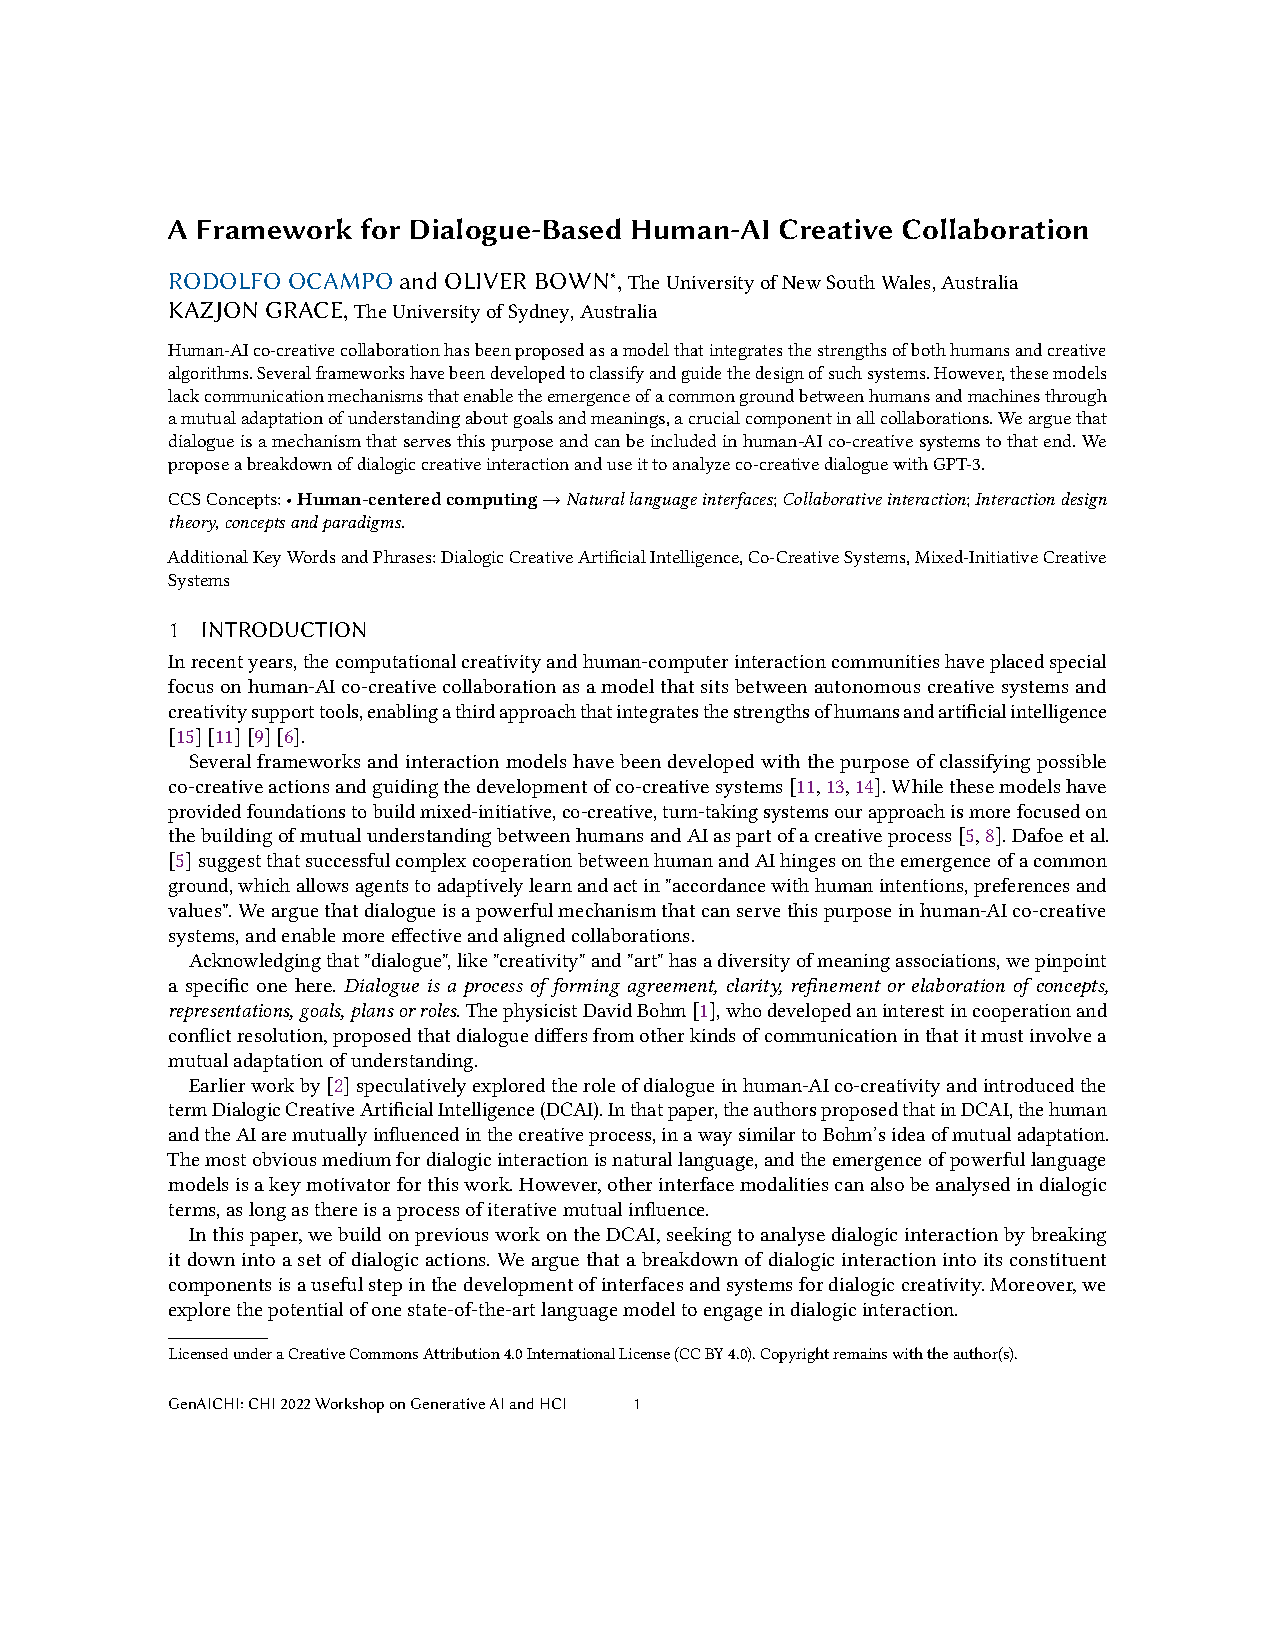
\includepdf[pages=-]{4-techchapter/GenCHI-thesis.pdf}

\section{Defining Dialogic Interaction as Human-Computer Interaction Concept}

Dialogue has been widely discussed in the context of human-computer interaction, mixed-initiative systems and co-creative systems \cite{Allen1999-sr, Yannakakis2014-zs, Deterding2017-wh} as a means to model human-computer interaction, however, it is yet to be formalised as both a theoretical concept and an actionable concept for interaction design. This chapter builds upon that work and on previous work by \cite{Bown2020-oc, Bown2024-yx}. As a unique contribution, in this chapter I seek to distill the elements that comprise dialogic interaction and how each can contribute to more effective human-AI co-creativity, thus providing a theoretical foundation for dialogic co-creativity as an interaction design concept. 

Dialogic interactions are based upon communication, iteration, feedback, adaptability, and deeper engagement, while non-dialogic interactions involve simple instruction giving or one-way communication, the sort one might observe commonly in computer-use paradigms such as command-based execution of tasks. For instance, in a dialogic interaction a writer might brainstorm with a language model, draft a story, request feedback on the flow, and iteratively refine the narrative—co-creating a text that neither agent could have produced alone. In contrast, in a non-dialogic interaction, the user may prompt the model in a command-driven way, to write a whole story. In this case, the involvement of the user is limited, which research shows may lead to worse quality, skill loss, and reduced task enjoyment \cite{Abbas2024-sf, Heersmink2024-mk, DellAcqua2023-og}. 

How to enable such dialogic interactions? At first glance, the question may seem trivially answered by chat-based interfaces. However, as I will discuss below, while chat-based interfaces certainly enable aspects of dialogic co-creativity, there are other important elements of dialogue that are not supported by such interface paradigms.

\subsection{Dialogic Co-creativity}

In 2020, \cite{Bown2020-zn} presented a speculative exploration of dialogue in human-computer co-creation, defining it simply as an interaction in which both actors influence each other. More recently, in \cite{Bown2024-yx}, we introduced a more comprehensive and formal framework for dialogic interaction, distinguishing among three levels: pseudo-dialogue, weak asymmetric dialogue, and full dialogue.

In \textbf{pseudo-dialogue}, the human provides instructions to the computer, which then generates an output for the human to evaluate. The interaction remains largely one-directional, as only the human models the AI; there is no cycle of mutual influence or shared intentions, and the channels for iterative, context-aware collaboration are limited. By contrast, \textbf{weak asymmetric dialogue} allows for some degree of bidirectional communication, but the computational agent’s capacity to model the interaction space is constrained. Although the communication may flow both ways, the relationship largely reflects a client-producer dynamic, with limited reciprocal understanding.

Finally, in \textbf{full dialogue}, both the human and the computer actively model each other. They engage in bidirectional communication that is aware not only of the immediate conversation but also of the broader collaborative context. This iterative process continuously refines the creative output while also deepening the mutual understanding between human and AI. 

In the following sections, I examine the elements that characterise \textbf{full dialogue}. The absence of one or more of these elements corresponds to instances of pseudo-dialogue or weak asymmetric dialogue.

\begin{figure}
    \centering
    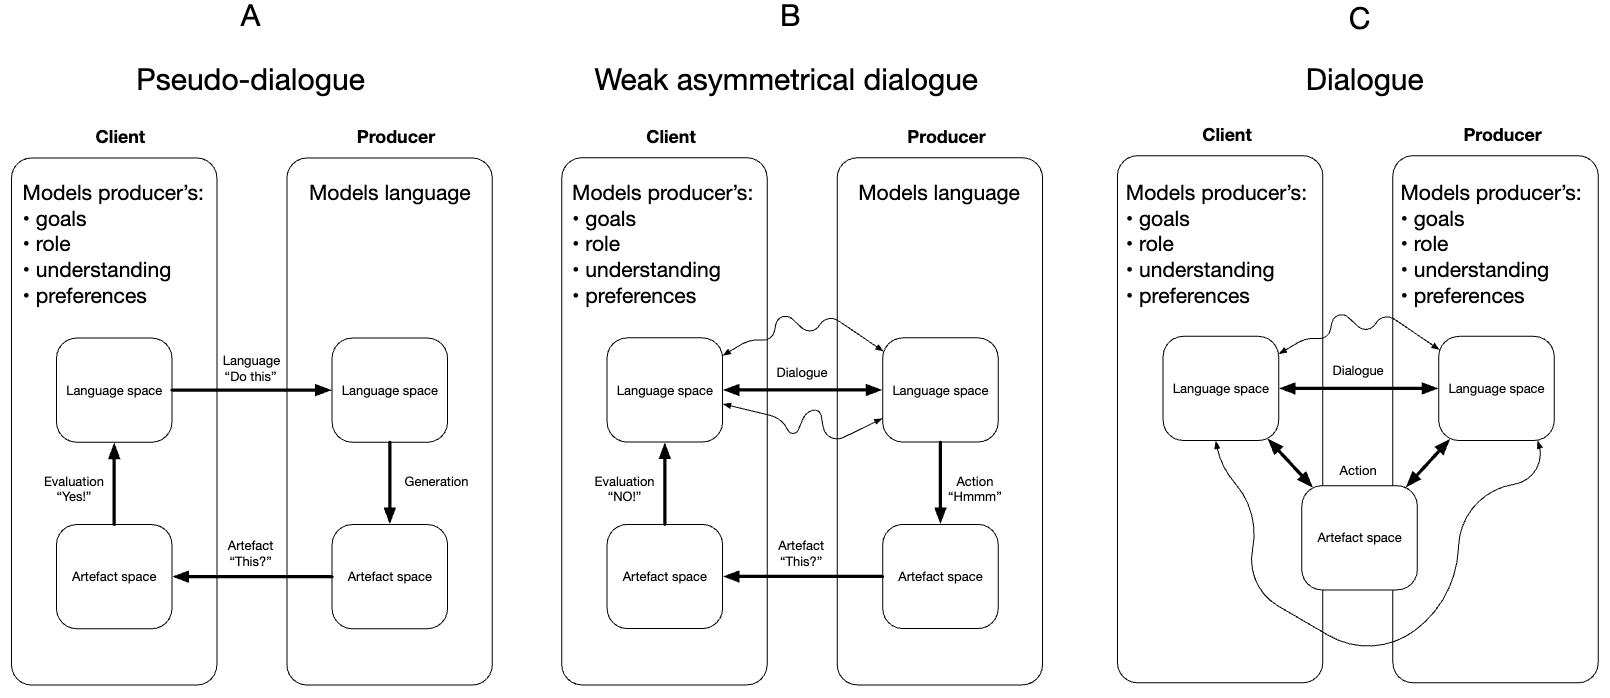
\includegraphics[width=1\linewidth]{levels of dialogue.png}
    \caption{Three levels of dialogic interaction. In weak-asymmetric dialogue, only the user models the AI who produces outputs based on prompts or requests. In pseudo-dialogue, a level of communication takes place but the collaboration and mutual modelling is limited. In full-dialogue, both model each other and act and evaluate the common creation.  Figure from \cite{Bown2024-yx}}
    \label{fig:enter-label}
\end{figure}
\subsection{Elements of dialogic co-creativity}

Drawing from the broader literature in philosophy, education, and HCI, I distil the following key elements of dialogic co-creative interaction. 

    \begin{itemize}
        \item Interaction \textit{through} and \textit{about} the creation, which involves: 
        \begin{itemize}
            \item Bidirectional Communication: Two-way communicative or conversational exchanges.
            \item A Shared Space: There is a common collaborative environment separate from instructions or chat interfaces.
        \end{itemize}
        \item Mutual Influence: Each party’s perspectives and goals evolve as a result of the interaction and each agent drives the other to new unexpected directions.
        \item Mutual Understanding: Each agent actively seeks to understand the other's world-models, goals, perspectives, preferences, etc.
        \item Iteration: The creative product and the shared meanings evolve iteratively.
        \item Context-awareness: Actors bring in the relevant context and act within it.
    \end{itemize}


    \begin{figure}
    \centering
    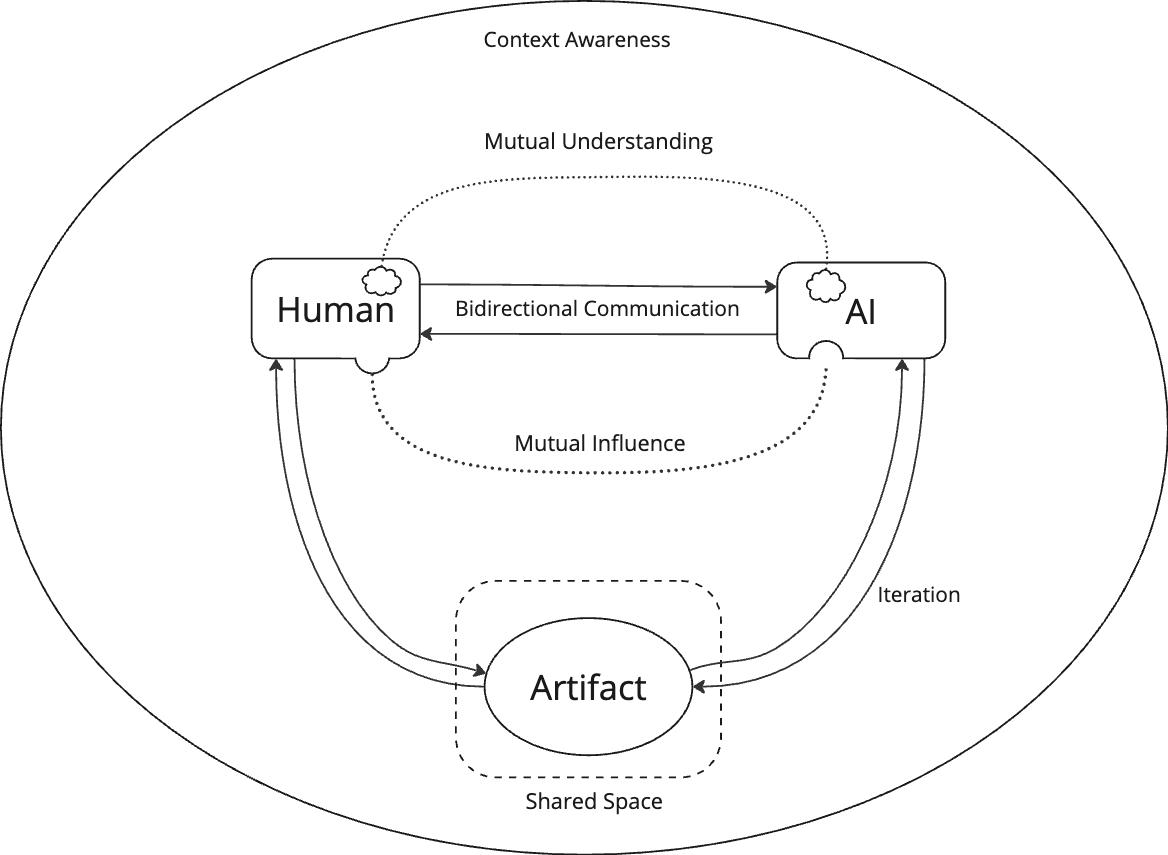
\includegraphics[width=0.75\linewidth]{dialogicelements.png}
    \caption{Dialogic co-creativity as an interaction design concept is comprised of six
essential elements: bidirectional communication, iteration, mutual influence, mutual understanding, shared space and context-awareness. }
    \label{fig:enter-label}
\end{figure}


In the next section, I elaborate on each element and discuss how each principle can improve human–AI co-creative outcomes, drawing on empirical evidence. By examining real-world examples and research findings, I highlight how dialogic features address frequent shortcomings of generative AI interactions—such as lack of nuanced steering, iterative dynamics and reduced user engagement.

\subsubsection{Bidirectional Communication}

One defining characteristic of dialogue is \textit{bidirectional communication}. Although such communication typically occurs through natural language, dialogue need not be constrained by verbal interaction alone. Etymologically, “dialogue” derives from the Greek words \textit{dia} (through) and \textit{logos} (word), yet several theorists maintain that dialogue can extend beyond mere language. For instance, the dialogic philosopher \cite{Buber1923-us} posits the possibility of dialogue occurring between humans and non-humans, while Donald Schön describes design as a dialogue among the creator, the materials, and the environment, in which iterative cycles of action and reflection incrementally shape the outcome \cite{Schon1987-fy,Schon1992-jt}. Within such a framework, dialogue functions as a cycle of mutual influence wherein information flows \textit{both} ways.

Other scholars, however, emphasize the importance of natural language for successful interaction between humans and sophisticated computational systems. Hayes and Reddy, in the early days of computing, advocated that "gracefully interacting systems" need to “conduct a dialogue in as human-like a way as possible,” highlighting the need to resolve linguistic ambiguity effectively \cite{Hayes1983-ca}. Much of their empirical work examined simpler systems lacking today’s advanced dialogic capabilities, but their core argument remains prescient: clear communication is critical for interacting with and understanding advanced systems.

\textbf{Empirical Evidence Supporting Bidirectional Communication}

Empirical support for the value of bidirectional communication in human–machine co-creation emerges from several studies. First, \cite{Rezwana2022-gg} compared two co-creative systems: one featuring bidirectional human–AI communication and another restricted to one-way (human-to-AI) interaction. Their findings showed that the bidirectional design improved user engagement, perceptions of the AI’s intelligence, and a more positive collaborative experience. Users reported that the AI felt more like a \textit{partner} than a mere tool, citing its ability to offer feedback and tailor outputs to user preferences. 

A second study, \cite{Ashktorab2021-ie}, investigated communication directionality in a cooperative game setting. The researchers found that systems capable of dynamically responding to user inputs—thus engaging in bidirectional communication—were viewed as more intelligent, likable, and conducive to rapport. By adaptively adjusting responses based on user prompts, the AI demonstrated a kind of non-verbal, iterative feedback loop. Conversely, systems with one-way communication were perceived as less cooperative and gave users a diminished sense of control.

A final, real-world illustration of two-way dialogic interaction is ChatGPT. The service, which became the fastest-growing consumer application—reaching 100 million registered users within two months and 300 million active users by December 2024—highlights the profound user appeal of conversational design. Notably, the underlying technology (GPT-3.5) had been available earlier, but as OpenAI President Greg Brockman explained in an interview when asked why ChatGPT became so successful, he claimed that ChatGPT’s interface was intentionally redesigned for \textit{dialogic} exchange. "we actually had the technology behind it (GPT3.5) the model behind it created almost a year prior so it wasn't new technology, the thing that we really did differently is that we did a little bit of extra work to make it more aligned so it really you could talk to it and it would do what you wanted, but secondly we made it accessible. We built an interface that was super simple. It was kind of the simplest interface we could think of." Brockman claims that the biggest take away is through this changes, they were able to "see the gap between what people thought was possible and what actually had been possible for quite some time" \cite{SXSW2023-wg}.Rather than merely offering text completions, ChatGPT was trained and fine-tuned (via Reinforcement Learning from Human Feedback, RLHF) to sustain a \textit{conversation}. 

\textbf{From Text Completion to Dialogic Interaction}

The evolution of GPT-based systems reveals a progression in dialogic interactivity. Early language models such as GPT-2 and GPT-3 operated in a predominantly \textit{text-completion} mode, offering no clear bidirectional exchange \cite{Brown2020-js}. Subsequently, \textit{instruction-based} models—exemplified by InstructGPT—enabled \textit{human-to-AI} communication by parsing user instructions \cite{OpenAI2022-pj}. Finally, with the introduction of ChatGPT, \textit{AI-to-human} communication also became formalised: the system now produces conversation-like “responses,” effectively completing a loop of bidirectional dialogue \cite{OpenAI2022-wx}.

\begin{table}[h!]
\centering
\resizebox{\textwidth}{!}{%
\begin{tabular}{|l|p{7cm}|l|}
\hline
\textbf{Interaction Model}         & \textbf{Description}                                                                                          & \textbf{Level of Communication}   \\ \hline
Text-Completion (e.g., GPT-3)      & No communication: The model completes text based on a provided input string. No back-and-forth communication. & None                             \\ \hline
Instruction-Based (e.g., InstructGPT) & One-way communication: The user provides an instruction, and the model completes it. Interaction is directive but linear. & Human-to-AI                      \\ \hline
Dialogic/Chat-Based (e.g., ChatGPT) & Two-way communication: The AI engages in conversational dialogue, responding to user inputs as part of an iterative conversation. & Human-to-AI and AI-to-Human       \\ \hline
\end{tabular}%
}
\caption{Progression of Communication Models in Generative AI}
\label{tab:communication_progression}
\end{table}

While chat-based, conversational, and dialogic language models have greatly increased the usability and adoption of AI-driven language technologies, they remain limited in their ability to serve as true co-creators. Among these challenges are the difficulty of detecting subtle nuances and fully grasping users’ intentions \cite{Bown2024-yx}, the propensity of models to fabricate information (“hallucinate”) \cite{Alkaissi2023-tp}, and the lack of dedicated spaces for co-creative processes beyond the chat interface \cite{Ocampo2024-dv}. In addition, these systems are not always sufficiently critical, often complying with user instructions despite erroneous underlying assumptions. I will return to these limitations in subsequent sections.


\begin{figure}
    \centering
    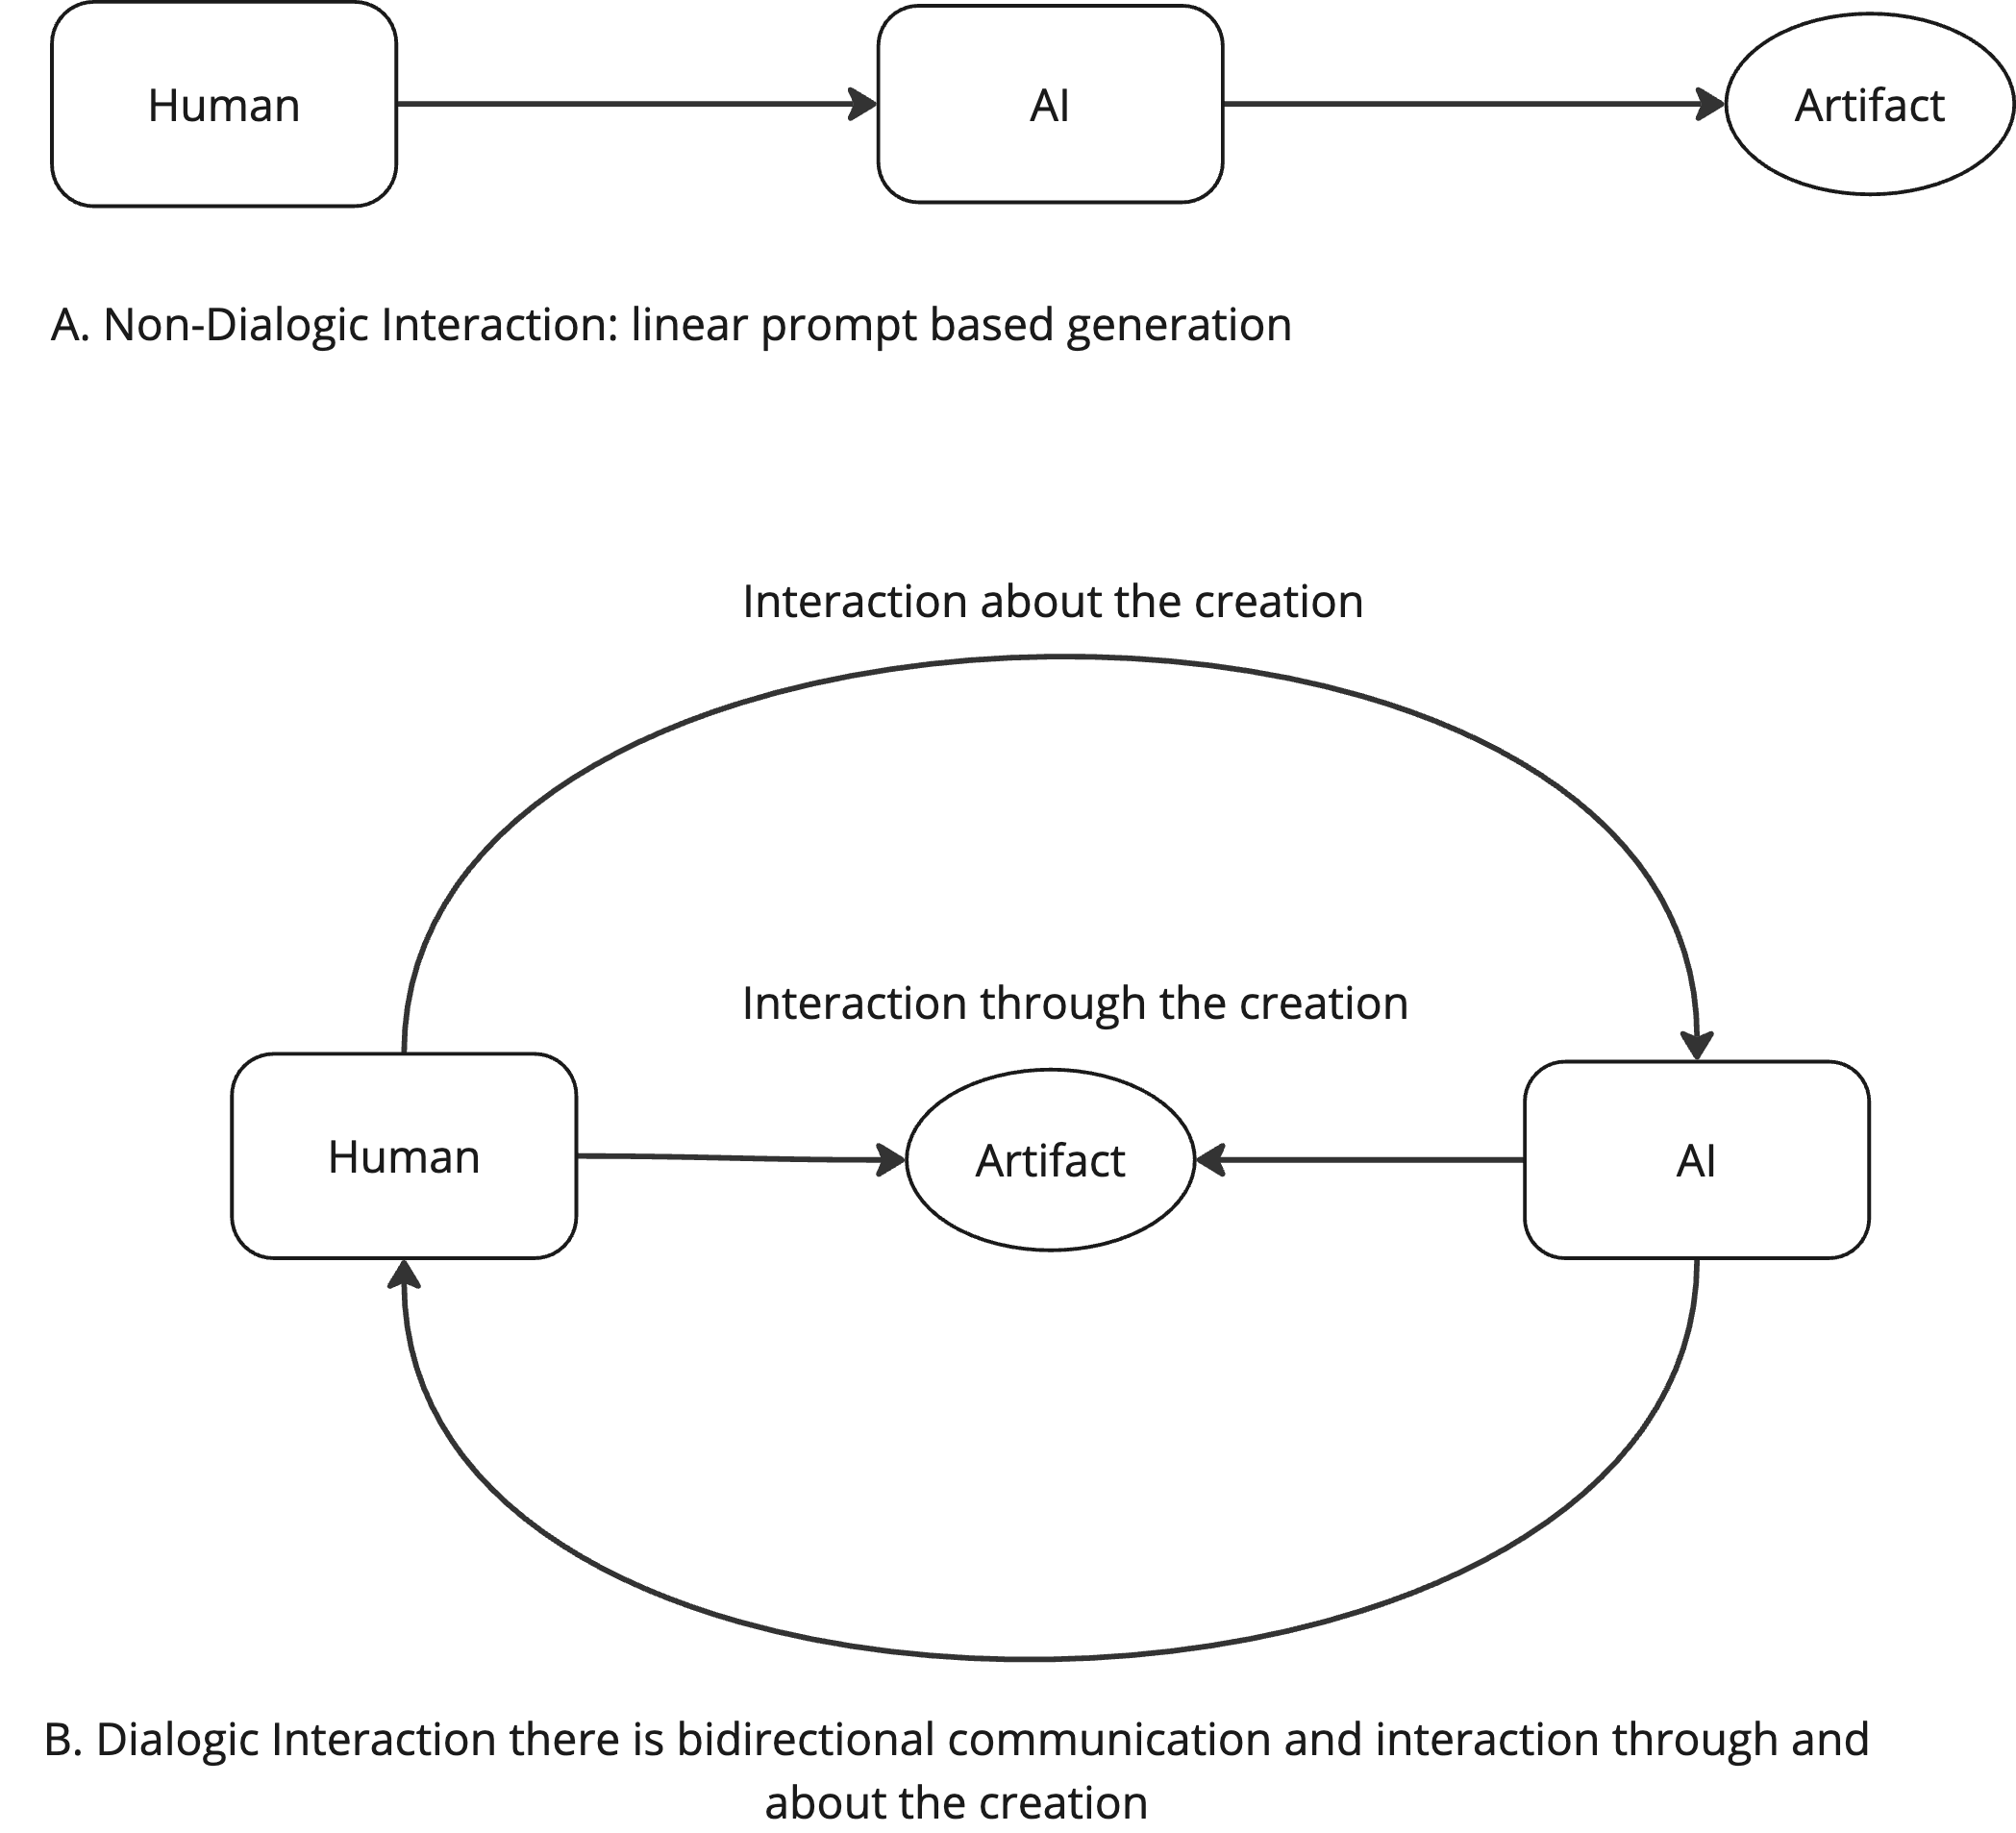
\includegraphics[width=0.75\linewidth]{Bidirectional.png}
    \caption{Interactions that enable two-way communication are important for effective co-creative dialogic interaction}
    \label{fig:enter-label}
\end{figure}

\subsection{Mutual influence}

Bidirectional communication is foundational for dialogic interaction, yet natural language exchanges alone do not guarantee effective co-creation. A key element is \textit{mutual influence}—the capacity for both parties to shape each other’s perspectives, goals, or actions \cite{Bown2020-zn}. In genuinely creative dialogue, participants provoke each other to reconsider their stances thus creating something \textit{new} that neither had created before the interaction. By contrast, non-dialogic exchanges exhibit limited mutual influence and primarily involve one-directional persuasion, as in giving orders, instructions, or arguing with the sole intention to convince.

A salient example of mutual influence in dialogue—and its importance for successful co-creation—appears in the Socratic dialogic method, one of the foundational applications of dialogue as an interaction technique. Unlike classical philosophical approaches such as sophist rhetoric or debates, whose aim was to persuade others of a particular viewpoint, the Socratic dialogic method functioned as a collaborative process of shared discovery. Socrates called his approach an “intellectual midwifery” designed to “give birth to a person’s inner wisdom” through critical thinking and the co-production of knowledge (although some dialogues ended in \textit{aporia}, or impasse) \cite{Nails2005-iq, Wikipedia-contributors2024-hr}. Participants typically began by posing a fundamental question, then iteratively questioned one another, proposed alternative viewpoints, refuted logically unsound positions, and ultimately arrived at a conclusion. The Socratic method was creative at two levels: first, it often, but now always, arrived at new philosophical solutions. More importantly, however, its aim was to modify the entrenched perspectives of interlocutors. Modelling this process is useful for enabling emergent creativity in human-AI interactions.

While some generative AI models demonstrate strong conversational abilities, they often fail to engage in questioning or actively seek to induce perspective shifts—except, for instance, when handling malicious queries. This behaviour is largely a result of alignment training for safety, in which models are optimised to comply with user instructions. However, in human-human co-creative dialogue, such reciprocal questioning and openness to influence are crucial.

A case study by \cite{Bown2020-oc} offers a practical illustration of how mutual influence shapes a creative process. In this study, two musicians co-created a song by offering alternative perspectives to each other. For instance, one musician (A) took a break and listened from outside the room. After hearing something interesting, he returned, declaring “That’s the hook!” Musician B, surprised, pointed to a different section and responded, “Oh, really, I thought \textit{that} was the hook.” B insisted, “No, no, \textit{that’s} the hook.” This exchange reveals how co-creators profit from actively exchanging viewpoints, prompting each participant to question their own assumptions. Tools like Oblique Strategies leverage a similar principle: they deliberately provoke shifts in perspective, offering oblique, unexpected suggestions that challenge the current framing. From the perspective of the psychology of creativity, this is particularly relevant, since one of the main obstacles in creative processes is hyperfixation in a particular solution or framing that leads to creative blocks \cite{Jansson1991-wy}. 

By contrast, most generative AI systems do not support this dynamic of mutual influence. More often, they conform to user instructions, potentially leading to less creative outcomes. Research has shown, for example, that ina  case study of image and design generation, using generative AI systems as part of a creative process led to greater fixation and less creative results than not using the system \cite{Wadinambiarachchi2024-jn}. 

Striking a balance between AI systems that actively question users and those that remain safe, aligned, and responsive is challenging. One promising direction may be to design systems that actively seek to introduce perspective shifts, and question the user productively, while allowing users to adjust parameters that govern this behavior. 

For example, consider a scenario in which a dialogic, multimodal co-creative musical AI system collaborates with a user composing commercial music. If the user plays a chord progression ending on a D\# in the key of E major and says, “Help me continue from here,” the system could move beyond simply following the prompt. It might propose a more adventurous move, for example: “What if, instead of finishing on D\#, you transition to an F\#7 to create additional tension? From there, we could resolve to a B major for an unexpected yet refreshing resolution.” This recommendation not only complies with the user’s request but also encourages rethinking—enriching the co-creative output.

Increasingly, interactive systems that incorporate some of these principles are appearing in both the literature and practice. For example, \cite{Kim2023-wt} describes the Scraft co-creative writing tool, which uses a language model as a “thought-provoking” tutor. It employs a Socratic questioning style to guide students toward deeper thinking and improved writing skills. Similarly, in “Do Make Me Think!” \cite{Reicherts2020-up} demonstrates how conversational interfaces that challenge users can scaffold cognitive processes, enabling them to discover new perspectives or previously overlooked trends. In 2019, \cite{Karimi2019-io} introduced a co-creative system for drawing that actively seeks to introduce novelty and perspective shifts by intentionally varying the visual and conceptual similarity with increasingly more novelty 

Mutual influence depends greatly on each party’s willingness to be influenced rather than simply to influence the other \cite{Bohm1996-fo}. Systems that question users to stimulate critical thinking and promote reciprocal engagement may help offset the risks of skill and critical-thinking erosion associated with overly compliant generative tools \cite{Abbas2024-sf, Essel2024-qc}. Nevertheless, the task is to achieve an appropriate balance between challenging users and following their instructions.

On the other hand of mutual influence is the influence flowing from the human to the AI. In what ways does the human influence the AI? In a seemingly trivial case, they exert influence merely by inputting prompts and requests thus producing an output by the AI. However, this seemingly trivial case actually disguises the more complex problem of control and steerability in generative systems, which I cover in more detail in subsequent chapters.

\subsection{Mutual Understanding}

A further essential facet of dialogic interaction is \textit{mutual understanding}, which Bohm describes as the process of modeling each other’s perspectives \cite{Bohm1996-fo}. Whereas mutual influence entails shaping each other’s views or actions, mutual understanding involves establishing a shared conceptual frame. Dialogue, in this sense, serves as a pathway to aligning and generating new, \textit{common} meanings. In his influential work on dialogue, Bohm posits that co-creativity emerges in the space where these new meanings form \cite{Bohm1996-fo}. Participants enter a dialogue with different worldviews—variations in how they define and interpret concepts—and these discrepancies can impede collaboration. Dialogue can rectify these misalignments, forging a common ground from which genuinely co-creative outcomes can arise.

Translating this principle to human–AI co-creativity highlights how both humans and AI bring distinct world-models into an interaction. Humans draw on lived experiences, while AI relies on patterns learned from vast training data, encoded within latent spaces. Inevitably, differences in how each interprets or values certain concepts can lead to misaligned objectives or aesthetics.

For instance, imagine a user prompting an AI to generate an image of a “beautiful house.” The system then produces a sleek, modern design, but the user—who prefers rustic, cozy homes—objects, remarking, “No, that’s ugly! Generate something made of wood, resembling a cabin.” In an ideal scenario, the model would learn that the user associates modern architecture with ugliness and rustic aesthetics with beauty. Yet many current generative models have limited capacity to internalise these user-specific preferences. In another example, \cite{Bown2024-yx} showed that model was unable to succesfully grasps the user preference for "witty" and sarcastic styles for crafting a tagline, significantly limiting its ability to successfully help the user. 

On the other hand, user's understanding how the system works is equally important. Research on \textit{explainable AI} suggests that systems capable of clarifying their reasoning or representations foster more effective interactions and user trust \cite{Ribeiro2016-xb,Doshi-Velez2017-qv}.

Significantly, mutual understanding need not be confined to verbal communication. Humans and AI can learn from each other iteratively through the creative process itself. In image generation, for example, the AI’s latent space determines how conceptual attributes (e.g., style, structure, or mood) are encoded. Co-creation may be viewed, then, as a form of \textit{latent-space exploration} \cite{Loh2024-fb,Smith2022-dm}, yet users often lack a concrete map of how to navigate these underlying representations. Some approaches attempt to render latent spaces semantically navigable, allowing users understand it and thus succesfully explore it \cite{Prathyush2024-ly, Harkonen2020-eu, Davis2024-ml}. By exposing the latent space in a more interpretable manner, these interfaces help users build more accurate mental models of the system.

Conversely, the system can learn (or at least simulate learning) about user tastes and implicit goals. For example, \href{app.leonardo.ai/}{Leonardo’s Flow State} prototype presents a grid of image variants; users pick one they like, then generate similar versions, effectively drilling deeper into the region of the latent space that aligns with their preferences. Such iterative sampling and selection not only refines outcomes but also promotes mutual understanding by enabling the AI to \textit{adapt} to the user’s evolving sense of aesthetic goals and constraints.

\subsection{Iteration}

Iteration is a key aspect of dialogic interaction, whereby participants take turns contributing and collaboratively refining ideas or outputs. Similarly, iteration underpins creative processes, as creators progressively refine their work through divergent and convergent stages. However, generative AI currently lacks robust mechanisms for iterative interaction, limiting its potential as an effective co-creative system. Indeed, a deficiency of iterative dynamics is frequently cited as a core constraint on generative AI’s co-creative utility, particularly in non-text-based tasks such as image creation \cite{Park2024-gw, Ocampo2023-gu, Peng2024-tr}. Consequently, designing iterative capabilities remains critical for advancing human–AI co-creativity.

The evolution of large language models (LLMs) illustrates the potential of iterative interaction. Over time, LLMs have progressed beyond non-communicative modes and one-way text completion toward dialogic, iterative modalities. These modes enable users to refine outputs by requesting modifications, expanding the AI’s suggestions, or clarifying goals. Nevertheless, significant limitations persist in these iterative processes \cite{Bown2024-yx, Ocampo2024-dv}.

At present, non-text-based generative systems lag behind LLMs in their ability to support iterative dynamics. This gap arises from both technical constraints and interaction-design challenges related to maintaining consistency, control, and refinement of outputs \cite{Ocampo2024-dv}. Consider, for example, a designer seeking to modify a newly generated sofa design. While the designer might like the core design, they may wish to make the sofa thinner or alter certain features. However, simply requesting such specific changes is rarely feasible: the designer can only attempt to re-prompt using the existing output as a reference, which may or may not yield a satisfactory result. Although emerging approaches—such as InstructPix2Pix \cite{Brooks2022-vo} and omnimodal foundational models \cite{Pichai2024-ao}—aim to address these issues, truly robust iterative refinement remains elusive.

From an interaction-design perspective, however, iterative dynamics are already achievable by structuring tools and workflows around multiple rounds of refinement \cite{Koch2020-gx, Lee2022-rj, Kim2023-wt}. For instance, systems can provide explicit feedback loops, where outputs become inputs in subsequent iterations.

Park et al. \cite{Park2024-gw} demonstrated that an exploratory GAN-based tool can better facilitate iterative image refinement than a single-step, text-to-image system like Stable Diffusion. Lee et al. \cite{Lee2022-rj} further showed that emphasising iterative interaction (rather than one-shot outputs) yields richer insights into users’ co-creative experiences. In a complex consulting task, Dell’Acqua et al. \cite{DellAcqua2023-og} found that consultants who engaged in tight, iterative feedback loops with an AI model outperformed those who interacted sporadically or relied on one-step solutions. Overall, the usability of generative AI depends heavily on its capacity to foster iterative dynamics, highlighting the importance of dialogic interaction in co-creative contexts.

\subsection{Shared Space}

Dialogic co-creation relies on a shared space in which participants can collaboratively contribute and refine artifacts. Paulo Freire, a central figure in dialogic education, emphasises the importance of dialogic space as a cornerstone of his pedagogical method \cite{Freire1970-pa}. How might this apply to human-AI co-creativity?

Consider the example of a writer collaborating with a chat-based language model, such as Claude or ChatGPT. The writer might begin with an initial draft and ask the AI to improve it. To further refine the text, the user must copy and paste the updated content back into a text editor, make any changes, and—if they wish to continue working with the model—reinsert the revised text into the chat. This repetitive process introduces significant friction, often discouraging the user from fully participating in iterative co-creation. Instead, they might accept the AI’s first suggestion and move on, leading to potential overreliance and a diminished sense of ownership. Evidence suggests that minimal user involvement can result in decreased performance, loss of personal style, skill erosion, and increased errors \cite{Abbas2024-sf, Rafner2021-tm}.

In two studies conducted across 2023 and 2024 during my doctoral research, I explored the impact of an interface I designed that offers both a chat window and a collaborative writing space shared by the user and AI. In this environment, both the user and the AI can read, write, and edit the text. Compared to conventional chat interfaces, this setup increased user involvement and strengthened their sense of ownership. It also shifted the collaboration dynamic away from a client-producer model, in which tasks are “outsourced” to the AI, and toward a more reciprocal co-creative relationship \cite{Ocampo2024-dv}.

Recently, chat-based AI tools have begun introducing features that support a shared space more seamlessly. For instance, Claude’s “artifacts” feature provides a dedicated area for text and code separate from the main chat window; however, the user cannot make changes in this space, only the AI can \cite{Whitney2024-pp, Anthropic2024-dl}. ChatGPT’s “Canvas” likewise creates a co-creative workspace where user and AI can jointly read, write, and edit text-based content \cite{OpenAI2024-ug}. These emerging designs represent early steps toward more robust shared spaces that foster deeper, more integrated human-AI co-creativity.

\subsubsection{Context Awareness}

A final crucial component of dialogue is what I refer to as context-awareness. Dialogic exchanges are interpreted not only in light of the immediate interaction but also through broader contextual factors. For example, Lucy Suchman \cite{Suchman2006-bs} illustrates how even a seemingly straightforward question—“Are you going to be here in ten minutes?”—and the response “Go ahead, take your break” rely on a larger contextual understanding implicitly known and not expressed in the current conversation. 

Similarly, creative practices are embedded within networks of meaning that extend beyond the present co-creation. Under an evolutionary lens of creativity, individuals respond to environments that are socially, culturally, and technologically constructed \cite{Bown2021-os}. Competencies to act within these environments include factors such as taste and trend awareness, alongside more practical artistic skills.

Consequently, a successful co-creative dialogue between humans and AI must be properly situated within the relevant context, which can happen at different levels. On one level, it may involve contextual awareness of past interactions, as well as the context awareness of the user workspace including previous works, files, context and preferences. On another wider level, it can involve a broader cultural context including awareness of current trends and social considerations that inevitably shape creative processes and the value of artifacts.

Consider for example, a designer using a co-creative image generation system to ideate designs for a fashion collection. Ideally, the designer would be able to reference their own style and past collections, as well as generating designs that are aware of the seasonal trends. Currently, the capacity for image generation systems to enable this is limited.

Consider a second example: a programmer collaborating with an AI language model to write code. In this case, ideally, the AI is integrated into the coding environment so that it can be aware of the existing codebase, dependencies, and the ability to create new files. 

\begin{figure}
    \centering
    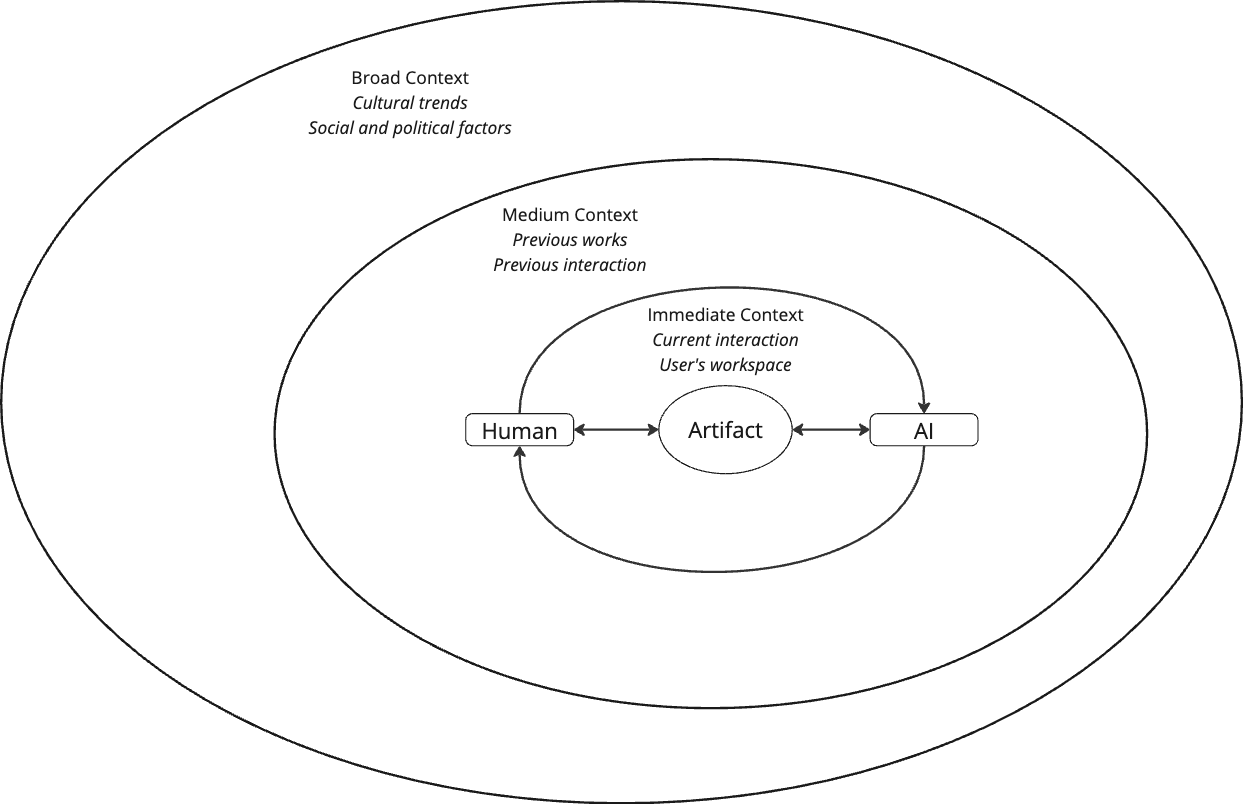
\includegraphics[width=0.75\linewidth]{context.png}
    \caption{Effective co-creative dialogues consider context at different levels}
    \label{fig:enter-label}
\end{figure}

Several emerging AI tools are advancing toward context-awareness and integration to varying degrees. \href{https://www.cursor.com/}{Cursor}, \href{https://v0.dev/}{v0}, \href{https://replit.com/ai}{Replit’s AI agent}, and \href{https://github.com/features/copilot}{GitHub Copilot} integrate directly into coding environments, enabling them to reference relevant files, generate new code, create additional files, and even handle deployments. \href{https://www.canva.com/}{Canva’s DreamLab} and \href{https://www.adobe.com/au/products/firefly.html}{Adobe} introduce generative AI within design workspaces, facilitating context-aware functionality. Google’s Gemini Workspace similarly seeks to integrate its features into users’ workflows across email, documents, and other files.

Achieving broader and more nuanced sociocultural context-awareness remains especially elusive. As part of an experimental, practice-based exploration of context-awareness in co-creativity (described in subsequent chapters), I conducted two new media installations that employ large language models (LLMs) to generate soundscapes based on environmental data. In one case, commissioned for the ANU School of Cybernetics, a soundscape was generated in response to data from the weather in Canberra, Twitter activity, economic indicators, and atmospheric CO2 levels. In another, commissioned for the Sydney Opera House, an LLM produced a continually evolving, month-long soundscape driven by data on the building’s energy usage, performances, and water consumption. In both instances, the role of the AI was to produce an on-going dynamic piece that directly responded to its context, be it the building, or the wider environment. To achieve so, maintaining relevant information within context, as well as the overarching goals and artistic intent, was crucial—and often challenging— for the installations.

In sum, meaningful context-awareness remains a crucial frontier for achieving successful dialogic co-creation with generative systems. Such systems must not only generate, iterate, and communicate but also function as situated agents within contexts of varying scope, relevant both to the user’s immediate workspace and to broader sociocultural webs of significance.

\subsection{Conclusion}

By drawing from the theory of dialogue and human-computer interaction, I have constructed a set of elements that characterise dialogic co-creativity as an interaction design concept. Table \ref{tab:dialogic_elements} offers a summary of these dialogic elements and their potential.  My proposal is that these elements can enabling effective co-creativity between humans and AI, ultimately leading to creative outcomes that neither part could produce alone. 

These elements form the basis of my analysis in subsequent chapters. By looking at my practice-based research case studies, user research study and the literature, throughout the rest of my thesis I will examine the impact of these elements and the challenges in implementing them to design effective co-creative systems.  

\begin{table}[htbp]
\centering
\resizebox{\textwidth}{!}{%
\begin{tabular}{|p{6cm}|p{11cm}|}
\hline
\textbf{Dialogic Element} & \textbf{Description} \\ \hline

Interaction both through and about the creation, which involves:

\textbf{Bidirectional Communication} 
& Two-way communication exchanges are crucial for dialogic interaction in humans and they can contribute to enhanced perceptions of collaboration and greater usability of generative models. \\ \hline

\textbf{Mutual Influence} 
& Effective co-creation between people rely on mutually influencing perspectives and goals. Co-creative AI can benefit from actively seeking to productively question, suggest, and move the user into new directions rather than simply following instructions. \\ \hline

\textbf{Mutual Understanding} 
& Dialogic processes involve aligning internal world models and meanings. Co-creative AI systems can provide more effective interactions by making themselves explainable to the user, and by actively seeking to model and adapt. \\ \hline

\textbf{Iteration} 
& Dialogue is an iterative process. Co-creative AI systems can provide more effective experiences if they enable users to iterate on outputs, as this is a common requirement and an important aspect of creative processes. \\ \hline

\textbf{Shared Space} 
& In creative dialogues, having a common collaborative space is important (shared text editors, DAWs, Canvases). Co-creative AI's can benefit from separating communication from creation and enabling a dedicated space for co-creation where both AI and user can see and edit the creation. \\ \hline

\textbf{Context Awareness} 
& The capacity to incorporate and respond to the broader context—be it the user’s immediate workspace, historical interactions, or sociocultural factors. \\ \hline

\end{tabular}%
}
\caption{Summary of Dialogic Interaction Elements for Human–AI Co-Creativity}
\label{tab:dialogic_elements}
\end{table}

\textit{In dialogic co-creativity, humans and AI engage in an iterative interaction with bidirectional communication in a cycle of mutual influence and understanding, while co-creating in a shared space and with awareness of the relevant context. }




    
\chapter{Beyond Chat: Collaborative Editors Enhance Human Involvement and Agency When Co-Writing with Large Language Models} \label{c:tc5} 


\section{Link to thesis}

This chapter addresses my core research question by focusing on interfaces that preserve \textbf{human creative agency}, examining \textbf{how interaction design shapes the roles of humans and AI in co-creative processes}, and informing \textbf{interaction design principles for effective human-AI co-creation}.

In a previous chapter, I conducted an initial exploration of dialogic interaction by adapting a text-completion language model into a conversational co-writer. There, I argued that effective dialogic co-creativity involves more than a simple two-way conversation; it requires interaction both \textit{through} and \textit{about} the creative product.

Between that early 2022 work and the paper presented in this chapter (conducted in 2024 and published in 2025) there was significant progress in generative language models. Indeed, interaction converged to conversational interfaces as the dominant paradigm. While these interfaces can facilitate dialogue to align understanding, I argue they predominantly support interaction \textit{about} the creative product, rather than \textit{through} it, simply because they lack the space to do so.

I hypothesised that an interface providing such a collaborative space could better support these two interaction modes. The research presented in this chapter tested this hypothesis through the iterative development of functional co-creative system prototypes in two versions, Vorges and Common AI. These systems combined a chat interface with a collaborative text editor, allowing the user and the AI to converse and edit a stateful piece of writing in separate but integrated spaces.

These prototypes were evaluated through two user studies, which provided empirical qualitative and quantitative evidence addressing my research questions.

Firstly, my \textbf{core research question} centres on designing generative AI interactions that effectively maintain human agency. Results demonstrated that chat-only interfaces restricted user agency and involvement at the writing level. In contrast, the hybrid interface, which combined a conversational and  a collaborative writing space, resulted in users reporting higher levels of agency and active involvement in the co-creative writing process.

Secondly, my research subquestion number one (R1) examines how interaction design influences the roles assumed by humans and AI in co-creativity. Findings indicated that chat-only interfaces typically positioned users in directive roles (providing instructions, requests, or initial ideas) while the AI predominantly occupied execution-oriented roles such as writer, wordsmith, or editor. Conversely, the hybrid interface encouraged a more balanced distribution of roles, with users more actively participating in the writing itself.

Finally, the third research subquestion (R3) explores interaction design principles for effective human-AI co-creativity. This thesis contributes insights integrated into the design principles outlined in the final chapter:

\begin{itemize}
    \item The need for a collaborative workspace in addition to a conversational space.
    \item The need to clearly manage AI contributions to avoid conflicts and ensure that users can transparently review, accept, or reject AI-generated input.
    \item The critical need for clear visibility of system affordances.
\end{itemize}

While the primary goal of my research is to design effective human-AI co-creative interactions, these studies do not offer definitive conclusions regarding the overall efficacy of hybrid interfaces. For instance, users reported slightly higher enjoyment and satisfaction with the final writing piece when using chat-only interfaces, yet described greater immersion in the creative process with hybrid interfaces. This may suggest a nuanced relationship between user involvement and their critical assessment of outcomes. It could also reflect difficulties users faced in managing collaborative editing and AI contributions, or it might be coincidental, given the effect size in these question was small.

These findings highlight the need for further research into how alternative interfaces beyond chat interfaces can impact co-creativity, recognising that interaction designers must balance diverse, often competing objectives.


% --- Manually add the paper's structure to the Table of Contents ---
% Note: The section titles in your paper don't have numbers, so we omit them here for a clean look.
\addcontentsline{toc}{section}{Introduction}
\addcontentsline{toc}{section}{Related Work and Background}
\addcontentsline{toc}{subsection}{Human-AI Co-Creativity and Mixed Initiative Systems}
\addcontentsline{toc}{subsection}{Beyond Chat Interfaces for Co-Creative Generative AI Systems}
\addcontentsline{toc}{section}{Prototypes}
\addcontentsline{toc}{subsection}{Version One – Vorges}
\addcontentsline{toc}{subsection}{Version Two – Common AI}
\addcontentsline{toc}{section}{User Studies: Designing a Shared Creative Workspace and Examining its Effect on Human-AI Co-Creative Writing}
\addcontentsline{toc}{section}{Study 1}
\addcontentsline{toc}{subsection}{Context, Experimental Design, Participants, Task, Measures, Methods and Analysis}
\addcontentsline{toc}{section}{Study 2}
\addcontentsline{toc}{subsection}{Context, Participants, Study Design, Task, Methods and Analysis}
\addcontentsline{toc}{section}{Study 1 Results}
\addcontentsline{toc}{subsection}{Differences in work distribution and involvement}
\addcontentsline{toc}{subsection}{Qualitative Results: Understanding Perceived and Assumed Roles}
\addcontentsline{toc}{section}{Results Study 2: Refined Interface and Deeper Qualitative Insights}
\addcontentsline{toc}{subsection}{High Enjoyment and Involvement}
\addcontentsline{toc}{subsection}{Users Who Outsourced Most of the Work}
\addcontentsline{toc}{subsection}{Users Felt Higher Creative Agency}
\addcontentsline{toc}{subsection}{Greater Autonomy and Collaboration than Popular Chat-Based Tools}
\addcontentsline{toc}{subsection}{Interface Clarity and Action Affordances as Areas for Improvement}
\addcontentsline{toc}{section}{Discussion and Conclusion}


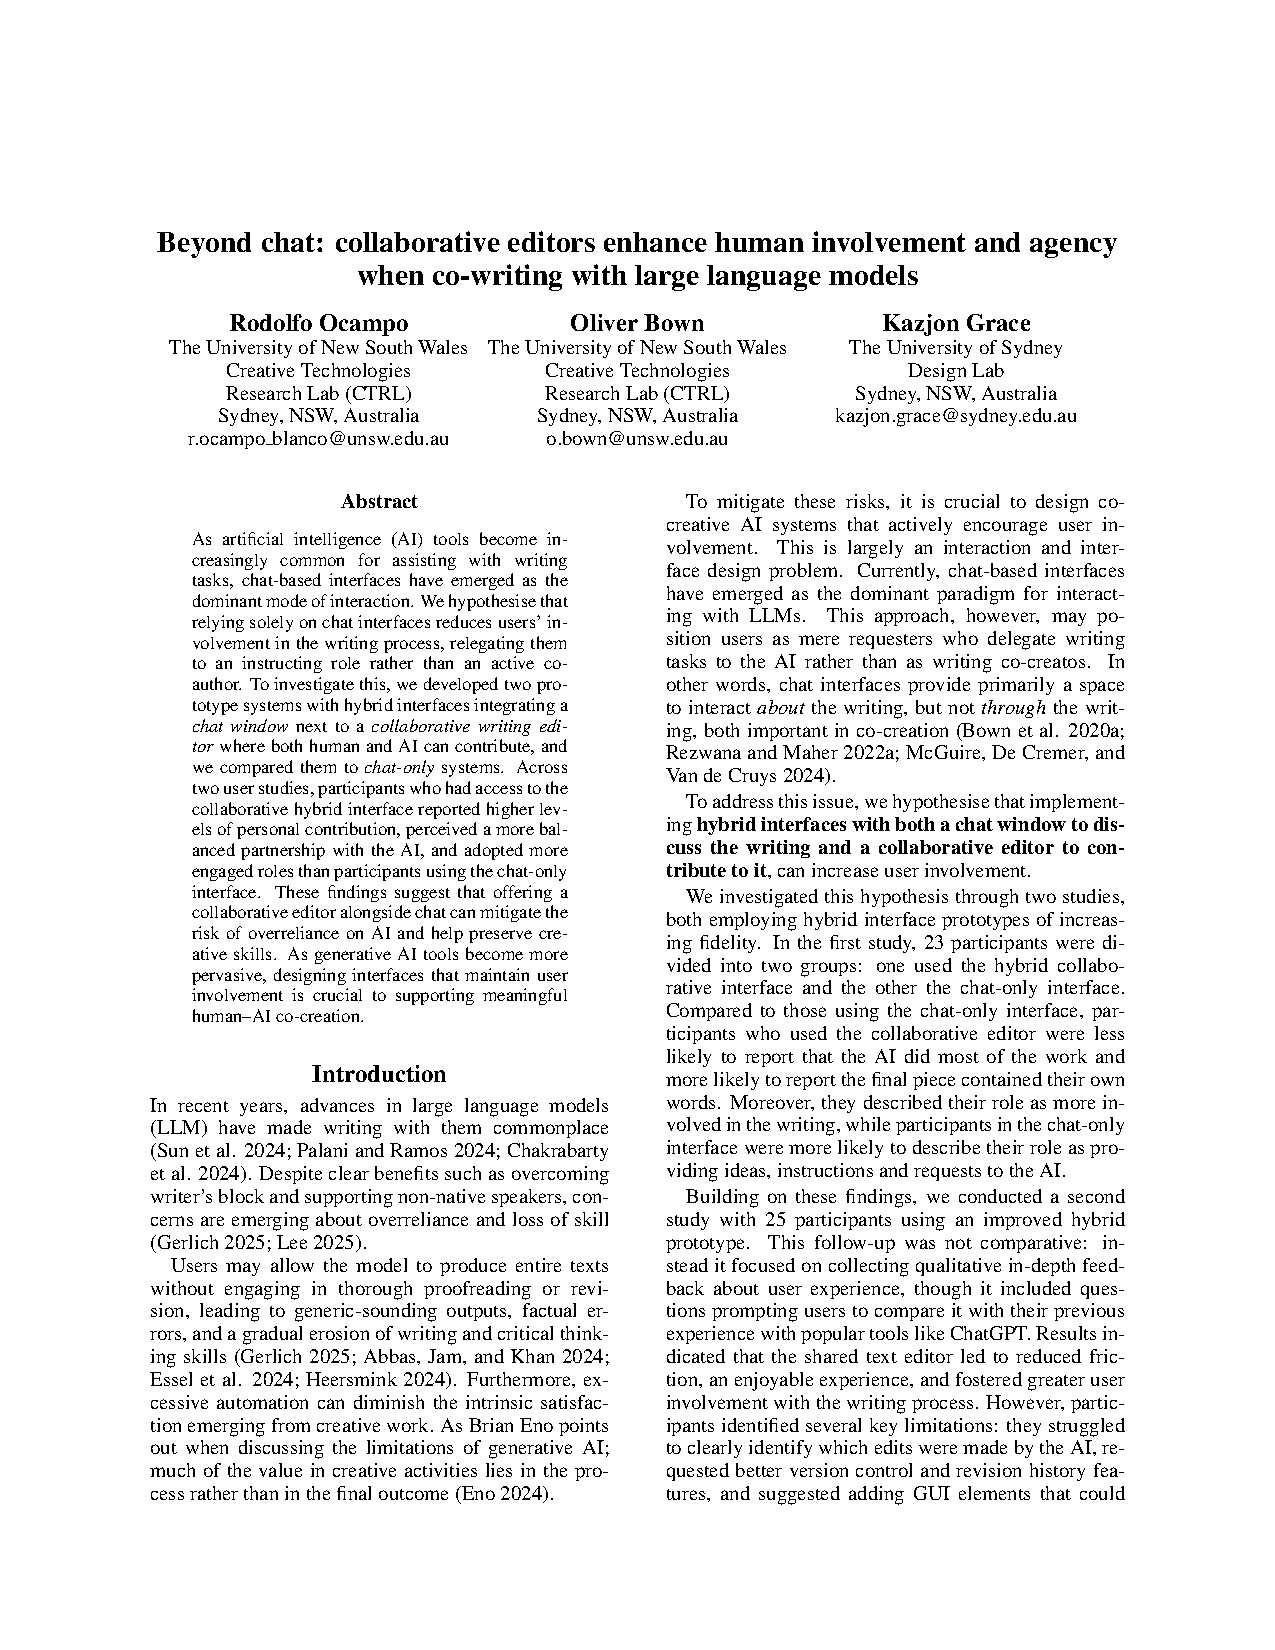
\includepdf[pages=-]{5-Writing/BeyondChat.pdf}

    \chapter[Human-AI Co-Creativity in Visual Production]{Integrating Generative AI into Creative Workflows: Dealing with Consistency, Scene Control, and Refinement in a Professional Image Generation Case Study
} \label{c:tc6} 

This case study shifts the focus to the domain of image-based generative AI, exploring research questions through a practical case involving real-world creative production. I collaborated with the Australian Financial Review to produce visuals for their annual Power Issue, which features “the most powerful people in Australia”. The aim was to produce “impossible photography” of the subjects, to tell stories about their personality and work in new ways, otherwise impossible with traditional photography. 

On one hand, this exploration contributes to understanding effective human-AI co-creativity by identifying how generative tools can enable new creative possibilities and use cases.

Secondly, a core objective of this case study was to examine the limitations of current tools in supporting real-world creative production. 

Findings from this work primarily inform my interaction design principles (R3) by highlighting crucial challenges. A significant limitation identified is the difficulty in enabling precise control over style and structure particularly when relying solely on prompting interfaces. A second notable challenge was iteratively refining promising images to pursue interesting directions. Exploring and further refining is a crucial dynamic in creative processes, and remains a critical challenge for successful human-AI co-creativity. 

This case study further illuminates ethical considerations. While the intention was partly to spark a debate around deep fakes, the discussion in this paper could itself help produce deep fakes. Moreover, tools that better integrate into creative production as argued here could lead to job displacements. Even if the intention was to explore possibilities not afforded by cameras, there is little preventing commercial usage to simply produce photographs passing as real: threatening the employment of models, actors, photographers and other occupations. 


\includepdf[pages=-]{7-techchapter/ICCC_short.pdf}


    \chapter[Artificial Intelligence as a Co-Creator in New Creative Practices]{New roles for generative AI co-creators: two case studies in new media public art installations}

\subsection{Link to thesis}
This last chapter presents two case studies exploring the potential of human-AI co-creativity in new media practice and public art generative installations. It is organised in two parts.

The first installation was commissioned by the School of Cybernetics at the Australian National University for their public exhibition: “Australian Cybernetics: a point through time”. A corresponding paper was presented at the 11th International Conference on Artificial Intelligence in Music, Sound, Art and Design (EvoMUSART) 2022 conference in Brno, Czech Republic.

The second installation was commissioned by the Sydney Opera House as part of their 50th anniversary celebrations, and a corresponding paper was presented at the Sound and Music Computing (SMC) Conference 2024 in Porto, Portugal.

Both installations were done in collaboration with music studio Uncanny Valley, and they explored the possibility of a new co-creative role for generative AI, particularly an LLM, in the context of data sonification. Specifically, the AI assumed the role of a semantic interpreter of semi-structured data corresponding to the surrounding environment where the installations were presented, and then translated this into an evolving audiovisual soundscape by controlling a music engine. Put simply: translating data from the environment into music in a creatively agentic way.

The core questions guiding the enquiry were: can generative technologies enable new forms of creative practice by assuming novel roles? How well can they fulfil these roles and what are the challenges involved in this type of creative practice? How can this inform my research questions relating to interaction design for effective co-creativity, human agency, assumed roles and dialogic interaction?

\subsection{New roles, new possibilities}

On one hand, experimental creative practice is a valuable research tool in interaction design \textbackslash{}cite\{Candy2019-vg, Vear2021-cx\} and creative technology \textbackslash{}cite\{Colton2012-jc, Cohen1995-wt, Cope2000-cq, Reichardt1968-eo\}. While generative AI presents the possibility to automate existing creative productions, both as an interaction designer and as a creative technologist, I am more interested in exploring its potential for enabling new creative possibilities. I believe this is where most of the co-creative potential between humans and AI lies. An emerging practice is increasingly exploring similar possibilities, as illustrated within the communities of practice in the venues in which this work has been presented, such as SMC and EvoMUSART. This work serves as a further invitation for interaction designers and designers of co-creative systems working with generative AI to explore what latent capabilities exist in these models, what new types of creative practice can they enable, and what new roles—roles that humans do not currently play—can these systems play.

In this case, I wanted to explore how a generative system, by virtue of turning complex data into a more digestible format (music) could serve as an interface with complex systems. This does not assume the need for a direct translation, as exists in the realm of data visualisation, but rather one that can draw the attention of the audience to the surrounding environment --be it a building, the weather, economic activity or atmospheric phenomena-- through its interpretation as a soundscape. Importantly: I explored the possibility of doing so in a semantically rich way, in contrast with sonification approaches that directly map values of the data to sonic qualities. 

\subsection{Generative variability, control and dialogue}

On a practical level, this installation illuminates challenges that have been echoed throughout this thesis and that are reinforced in the conclusion: the challenge of generative variability, where it is difficult to anticipate and predict what the model will do. In some cases, this merely involves the case of fixating on an output over and over, as described in the first paper, or the more visible case of outputting offensive material, as happened during one of the installations.

Addressing this in real time was challenging. Given that the model only worked by executing a generative task based on a system prompt, strategies were constrained to examining logs of inputs and outputs and tweaking the prompt accordingly in a limited attempt to steer future behaviour. This illuminates a potential opportunity for dialogic interaction. One can imagine a dialogic backdoor: a conversational interface where I could steer the model and ask, “why did you make this choice?” or suggest, “you have fixated on that particular element too much, try something different”.

\subsection{Context-awareness for situated co-creativity}


These installations also revealed the capacity for language models to bring in external context. And with this, create artworks that are socially situated. In theory, if the installations were presented elsewhere, the artwork would be different. Of course, this is the case simply because the outputs are ever changing, but it is the hope that the outputs at least would reveal some aspects of the environment they are surrounded by. For example, in the case of the Opera House installation, it was noticeable in the music when the building was empty late at night: the music was mostly calm. In contrast, during peak hours where there was considerable activity in the building, the soundscape became more energetic, sonically crowded and heavy.

Such interactions highlight an aspect I discuss as a part of dialogic interaction: context awareness. Regardless of the particular use case—traditional practices or experimental new media applications—bringing in the context offers new possibilities for more situated human-AI interactions.

\subsection{Agency, and the human as gardener}

Lastly, these installations also illuminate a crucial thread throughout my thesis: that of human agency, and the role we played in it. The soundscape produced in these installations was generated using a music engine that arranged, combinatorially, a set of human-made or human-curated music stems. The LLM controlled this engine through selecting some settings, based on interpretations of how best to map the data into the music (the details are provided in the papers).

As such, it can be argued that we, the team, maintained agency over the sonic quality of the outputs, maintaining involvement at the artefact level. Moreover, we constrained the possibilities of how sounds could be combined, to maintain compositional control and intent. This can be understood as a meta-composition, not directly composing the soundscapes but creating the building blocks and providing the constraints within which the AI operated. We engaged the creativity of the AI, in turn, to operate within these bounds and decide how the incoming data would be mapped to soundscapes. I believe this illustrates a promising possibility for human-AI co-creativity: that of ever-evolving pieces, in music, narrative or otherwise, where the human meta-composes, and the AI executes generatively.

Existing generative practices have explored this role of the “human as a gardener”. For example, Brian Eno’s generative practice based on applications of simple rules in music looping. But generative AI opens a possibility where more agency is handed to the AI to make decisions. It also affords the possibility of “talking to the system”—setting goals, aligning meaning—in contrast to previous generative practices where the generative system was a blind compounding of rules that afforded no natural language interaction.

Lastly, to clarify my involvement: I originally developed the approach of semantic sonification described here, and was in charge of the development and implementation for the generative AI, collecting the real-time data and feeding it to the AI components. Uncanny Valley was involved in the development of the music engine that the LLM connected to and controlled.

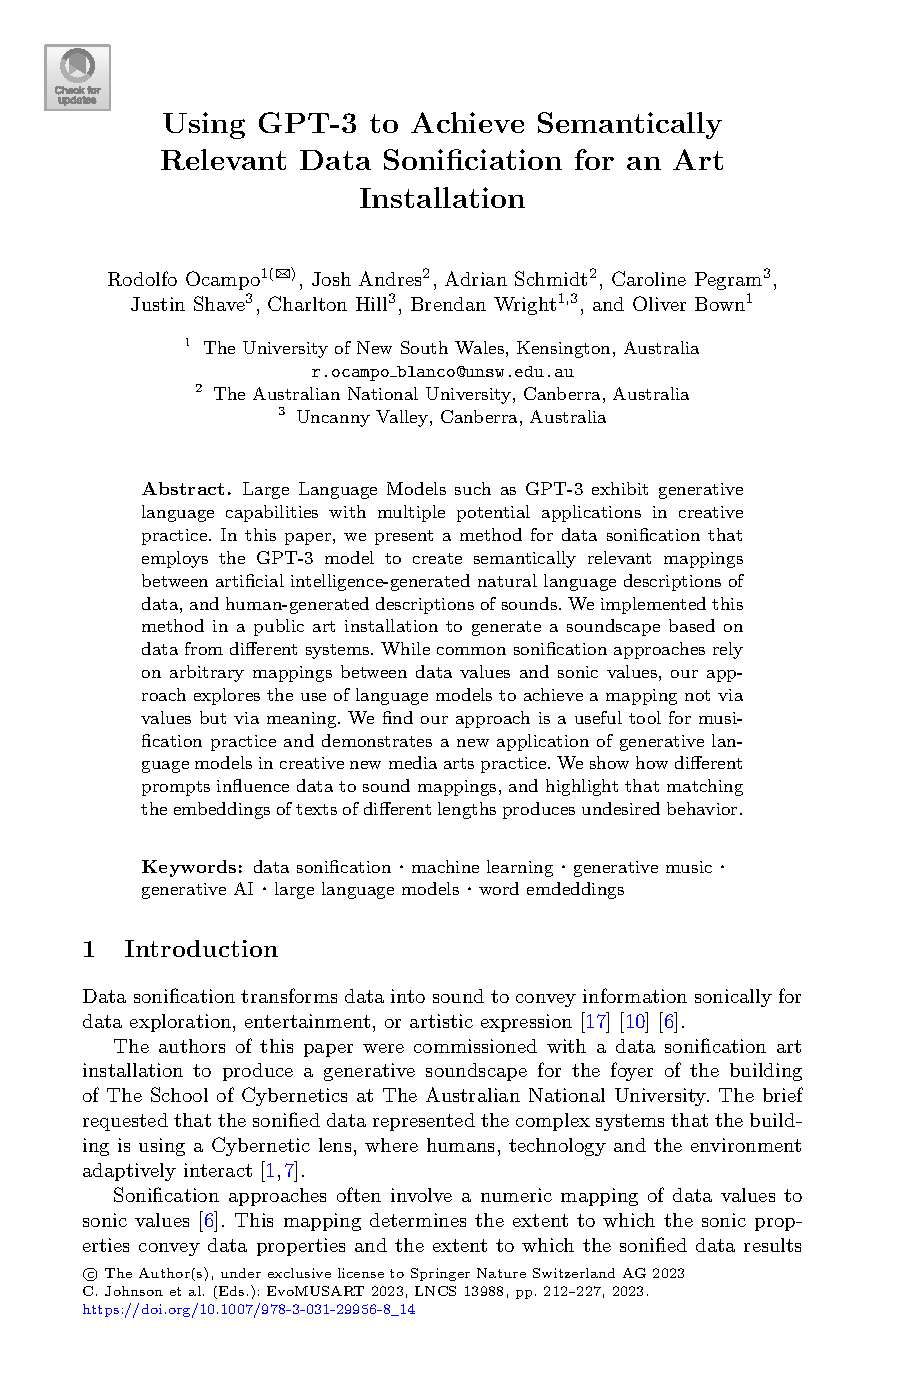
\includepdf[pages=-]{6-techchapter/EvoMusArtPaper.pdf}

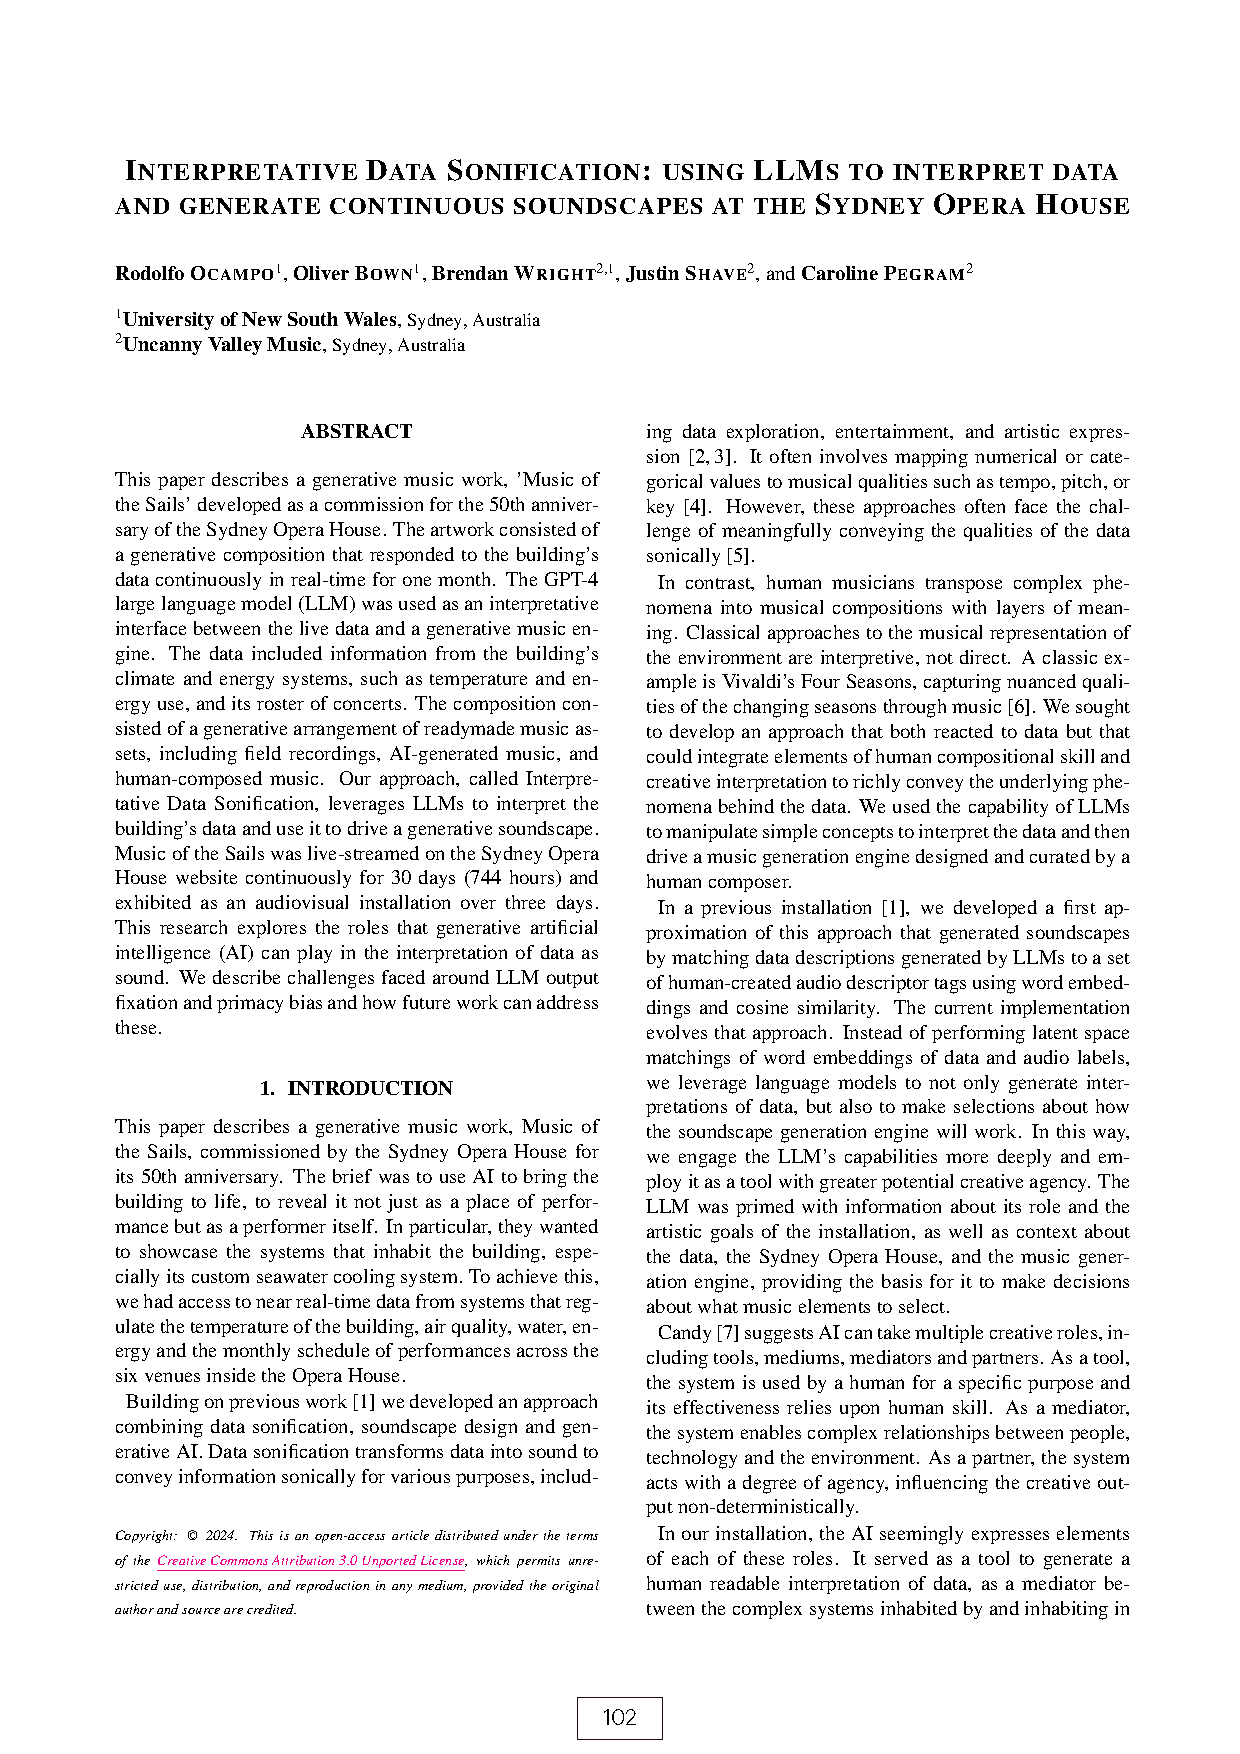
\includepdf[pages=-]{6-techchapter/SMCPaper.pdf}




    \chapter[Conclusion]{Conclusion}\label{c:conclusion}

The core aim of this thesis was to examine how to enable co-creativity between humans and generative artificial intelligence. Specifically, the following core research question was posed.

\begin{quote}
\textbf{Core Research Question:}
\emph{How can we design generative AI systems that act as effective co-creators, maintaining human agency while effectively leveraging the creative potential of this technology?}
\end{quote}

This was broken down into the following sub-questions:

\begin{quote}
\textbf{Sub-Questions:}
\begin{enumerate}
    \item \emph{Which interaction design principles can guide the development of effective co-creative systems?}
    \item \emph{What is the potential of modelling dialogue in interaction design to enable effective human--AI co-creativity?}
    \item \emph{How does interaction design influence the role that humans and AI play in creative production?}
\end{enumerate}
\end{quote}

I examined these questions through a mixed-methodology approach, developing and testing prototypes with users from a design research perspective, and engaging in creative practice through collaborations with teams working on real-world creative productions.

This chapter begins by presenting the core argument of the thesis. It then unpacks this argument by addressing the research sub-questions, starting with an analysis of how interaction design shapes the roles, agency, and effectiveness of human-AI interaction. Following this, I explore the potential of dialogic interaction to enhance co-creativity, culminating in a final section that synthesises these findings into a set of actionable design principles.

\section{Core argument}

This thesis argues that prevailing modes of interaction with generative AI in creative activities often diminish user creative agency through what I term \textbf{severed creative agency}: a fundamental disconnect between a user's creative intentions and the actions performed by the AI.

This severing emerges from a significant shift in role distribution. Humans increasingly operate within the \textit{intentional space}, where creative goals, visions, and high-level decisions reside, while AI systems take on roles in the \textit{action space}, where concrete artefact-level operations such as drawing, writing words, or playing notes occur. This division can ultimately lead to less effective interactions, where users struggle to translate their intentions into desired outputs. 

\textit{Dialogic design} is a promising approach to increase human agency and the effectiveness of human-AI co-creativity by more closely aligning intention and action in human-AI interaction. Dialogic design involves creating context-aware, iterative interactions that promote mutual adaptation and understanding. In such systems, humans and AI engage in bidirectional communication not only through language but also through the creative artefact itself. In the last section, as the core contribution of this thesis, I articulate a set of design principles that operationalise dialogic design, offering concrete guidance for the development of co-creative AI systems.

\section{How Interaction Design Influences Roles and Agency}

We can understand creativity as a process of moving between two distinct but interconnected spaces: the \textit{intention space} and the \textit{action space}. In the intentional space reside goals, taste, decisions, directions, and the intention to express. In the action space are the concrete creative acts: writing words, playing notes, or drawing lines—the actions performed at the artefact level. This distinction is found across the literature \cite{Palani2024-on} and I argue it is core to understanding the shifting of roles between humans and AI in creative activities.

\begin{figure}[H]
    \centering
    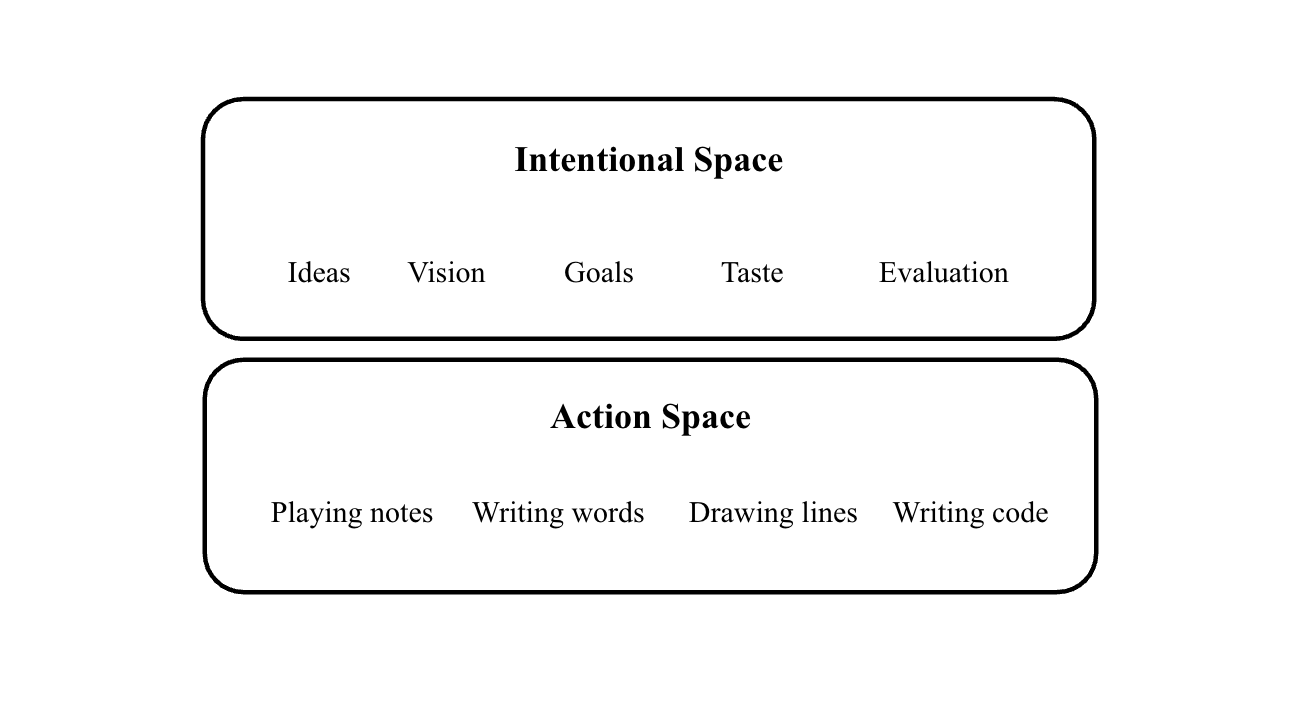
\includegraphics[width=1\linewidth]{intention action spaces.png}
    \caption{The distinction between the intention space (goals, vision, decisions) and the action space (artefact-level operations).}
    \label{fig:intention-action-spaces}
\end{figure}

The research in this thesis, alongside emerging literature, shows that when interacting with AI, humans largely assume roles in the intentional space while the AI assumes roles in the action space. In Chapter 4, I discussed how participants often described their roles in these terms, when interacting with a chat-based AI:
\begin{quote}
"I was the curator of the story—I picked the pieces I liked and left the rest."

"I gave it the idea, and it just took it from there, writing almost everything."

"I gave it the skeleton of the story, and Vorges fleshed it out, almost like giving the recipe and having it cook the dish." 

"I asked it to write a paragraph about a dystopian future, and it did everything from there." 

"I started with a basic introduction, and Vorges expanded it into a complete narrative." 

"Vorges wrote 90\% of the story based on my prompts. I just tweaked it a bit."
\end{quote}
People tended to describe their roles specifically as director, editor, or curator. This echoes similar findings in the literature. In an extensive review of emerging roles and workflows, Palani et al. \cite{Palani2024-on} found that users increasingly assume roles at the "Project" level while AI assumes roles at the "Artifact" level. This also aligns with professional practice. The emerging practice of \textit{vibe-coding} was described by AI researcher Andrej Karpathy as prompting an AI to write code, barely being involved in reading or understanding it:
\begin{quote}
"[I] forget that the code even exists. [...] I barely even touch the keyboard. [...] The code grows beyond my usual comprehension [...] It's not too bad for throwaway weekend projects, but still quite amusing. I'm building a project or webapp, but it's not really coding"
\end{quote}
As Weisz argues: "Generative AI technologies have introduced a new paradigm of human-computer interaction, what Nielsen refers to as “intent-based outcome specification”. In this paradigm, users specify what they want, often using natural language, but not how it should be produced." \cite{Weisz2024-io}.

This shifting of roles, where humans move into the intentional space and AI assumes roles in the action space, introduces a fundamental tension: a disconnect between intention and action. If we accept the standard definition of agency as \textit{intentional action} \cite{Schlosser2019-jk}, it is clear how this may affect human creative agency, especially given the difficulty of steering models, successfully getting them to do what we want, and understanding how and why they are doing it. I propose this could be described as severed creative agency.

\begin{figure}[H]
    \centering
    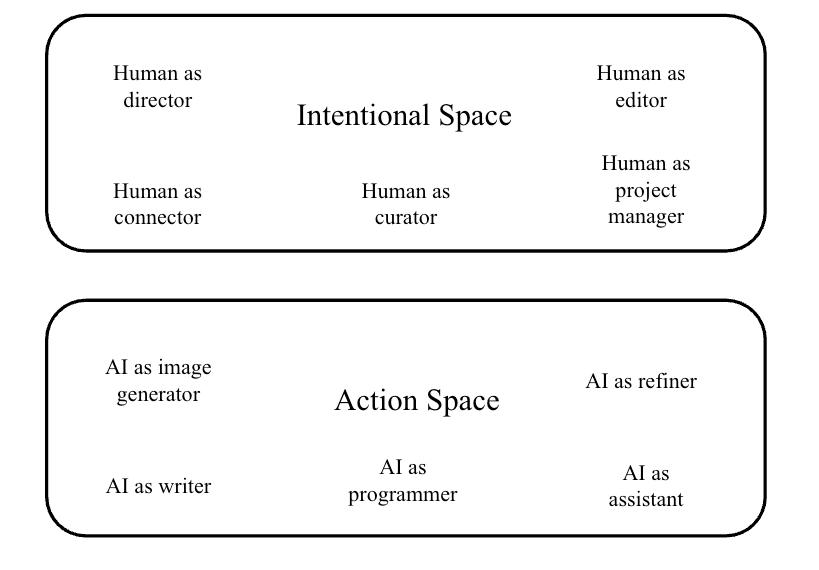
\includegraphics[width=0.75\linewidth]{roles.png}
    \caption{The distribution of roles in typical human-AI creative interaction, with the human operating at the intention level and the AI at the action level.}
    \label{fig:roles-in-spaces}
\end{figure}

\section{Severed Creative Agency}
Let's discuss further the effect of this separation between the intentional and action spaces, how this leads to severed creative agency, and how it contributes to our understanding of interaction design for effective human-AI co-creativity.

I argue it occurs primarily because of three reasons. 


\subsection{Failing to Align Instructions to Outputs}

Firstly, severed creative agency stems from the difficulty in controlling generative AI's outputs, which introduces a disconnection between intention and action. For example, in my case study with the AFR in Chapter 6, I identified the main limitation in our creative process was controlling generative AI image models, both stylistically and structurally, to achieve consistent results across iterations that allowed us to refine images towards convergence. Similarly, Palani et al., in the same study discussed before, found that two of the main limitations for adoption of AI in creative activities are: "Aligning and Assessing Stochastic Model Outputs With Intent" and "Articulating creative goals" \cite{Palani2024-on}. For example, one of their participants claimed:
\begin{quote}
"I was prescriptive in my prompt, and I thought I nailed it. But the model never did, and it still doesn’t. That drives me crazy and keeps me surprised, delighted, and sometimes annoyed."
\end{quote}
Another user described the challenge of articulation: "at times, I didn’t have the vocabulary to ask the model to help me. I think your background knowledge matters: someone with an art history background knows how to prompt a specific style, unlike someone who doesn’t." This difficulty is compounded when trying to articulate tacit knowledge such as style and expertise.

This is a notable feature of generative AI systems, which Weisz \cite{Weisz2024-io} terms "generative variability." While this can introduce surprise and delight, in serious creative production, it can lead to annoyance and unusable tools. Weisz argues: "With generative AI applications, users will need to develop a new set of skills to work with (not against) generative variability by learning how to create specifications that result in artifacts that match their desired intent." 

In the case study described in Chapter 6, in which I worked with a creative team in a professional setting to generate visuals for a magazine, after trying multiple tools, we settled for one that allowed us to pass images as reference for generation as the feature that most control allowed us to have. Similarly, a study by Peng et al. \cite{Peng2024-tr} with designers found that a multimodal interface, where users could provide images, colours and text to steer the generation, allowed them to "explore and express themselves more effectively." 

These results reflect a fundamental need: a study by Park et al. \cite{Park2024-gw} found one of the main struggles for designers using generative AI is expressing visual things verbally, and they highlighted the need for multimodal visual centric input interfaces where they could simply provide images as references. 

These findings could be extended to other domains: for example, a co-creative system in music could allow users to pass music as reference. But it also opens the door for other new types of creative operations. For example, passing an image as a "vibe" reference to generate music, such as the example shown in Figure \ref{fig:vibesynth}. While multimodal inputs are not entirely new, the latent spaces in generative AI models show significant symmetry between modalities and enable rich translations between them that were previously unavailable to creative practitioners \cite{Radford2021-hb}.  


\begin{figure}[H]
    \centering
    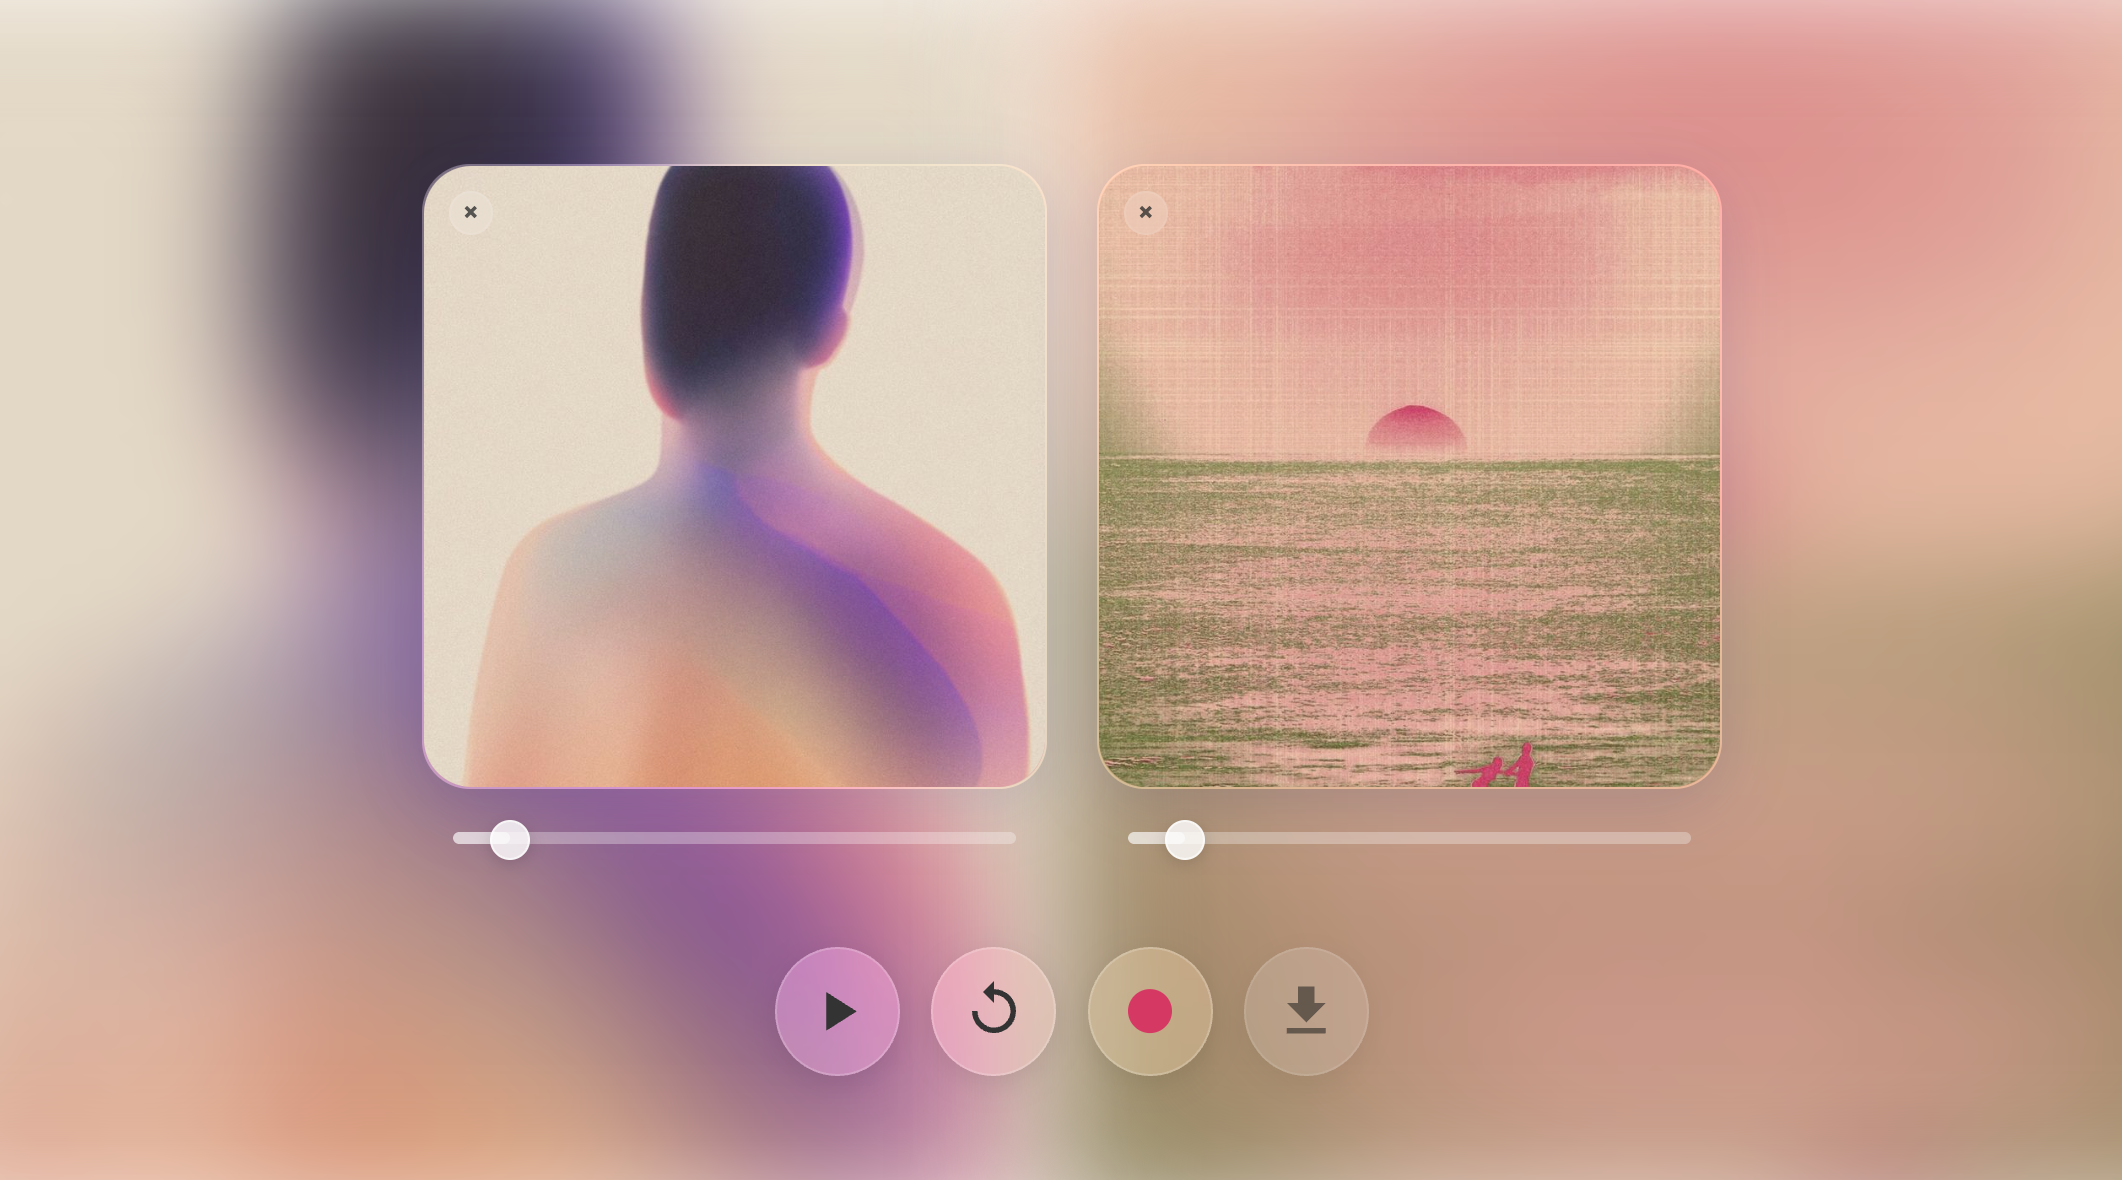
\includegraphics[width=.75\linewidth]{vibesynth.png}
    \caption{Vibesynth.ai, (https://vibesynth.ai/) a tool developed by the author that allows the user to pass images as reference for music generation and control the influence of each. This tool was developed outside the context of this thesis but serves as an illustration of multi-modal inputs for generative AI systems}
    \label{fig:vibesynth}
\end{figure}



\subsection{Erosion of Skills}
Secondly, agency is affected through the erosion of skills, limiting the confidence and ability of practitioners to turn their intentions into outputs. A growing literature finds that overreliance on AI to execute tasks can lead to critical skill loss \cite{Heersmink2024-mk, Rafner2021-tm}. Gerlich found that overreliance on AI for writing tasks is linked to a loss of critical thinking skills \cite{Gerlich2025-as}. A recent study by Lee et al. \cite{Lee2025-dw} found that the use of generative AI in knowledge workers was linked to less cognitive effort and reduced self-confidence. This is particularly concerning for creative agency, as creative self-efficacy, defined as confidence in one's creative ability, is a crucial determinant of creative achievement.

However, research also shows this is largely mediated by the level of user involvement at the artifact level. For example, a study by Kim et al. \cite{Kim2023-wt} found that a generative writing tool repurposed to act as a Socratic tutor, asking questions instead of merely writing, was able to increase students' writing skills. Similarly, a study by Essel et al. \cite{Essel2024-qc} found that using an LLM helped increase students' critical and reflective skills when they were provided with pre-written prompts to stimulate critical thinking. This shows that conversational design is an increasingly important tool in the interaction design toolbox, and a central one in the context of dialogic interaction.


\subsection{Erosion of Enjoyment and Involvement}
The third way the shift to the intentional space affects co-creativity is through the erosion of one of its core features: intrinsic enjoyment. Take the case of a participant in my Chapter 4 study, who described using the Vorges tool to write:
\begin{quote}
"[it] made me feel like I was cheating somehow. It does not feel like my work, even though I gave all the ideas. Also, I believe there is satisfaction in putting a lot of effort/dedication/patience into something. Vorges made everything so simple, fast, and easy that it felt artificial and no real satisfaction came as a result."
\end{quote}
A similar sentiment is echoed by artist and generative art pioneer Brian Eno \cite{Eno2024-rj}:
\begin{quote}
"In my own experience as an artist, experimenting with AI has mixed results. I’ve used several “songwriting” AIs and similar “picture-making” AIs. I’m intrigued and bored at the same time: I find it quickly becomes quite tedious. I have a sort of inner dissatisfaction when I play with it, a little like the feeling I get from eating a lot of confectionery when I’m hungry. I suspect this is because the joy of art isn’t only the pleasure of an end result but also the experience of going through the process of having made it. When you go out for a walk it isn’t just (or even primarily) for the pleasure of reaching a destination, but for the process of doing the walking."
\end{quote}
Compare this with a user in a second experiment in Chapter 4, using a prototype that afforded contributing at the action level via a shared editor:
\begin{quote}
"I really-really enjoyed writing this. I even had a deep moment of reflection, my writing was nostalgic and sad, but I was able to use AI to steer it in the right direction, it gave me confidence that I was also writing with correct grammar and spelling, English is not my first language and while I am proficient, I can still use proofreading to ensure good quality, this tool helped me with it." (P4 Common AI)
\end{quote}
Others shared this perspective:
\begin{quote}
P9 shared: “I liked how my original ideas were still retained, and AI was used to complement my intentions. It forced me to put in some effort and do the majority of the work.”

P22 emphasized: “It adds an element of working together, which I think is the moral problem with current AI tools—they often seem like they’re doing all the work.”
\end{quote}

In sum, focusing on the output rather than the process erodes intrinsic enjoyment and motivation, which is a crucial aspect of creativity \cite{Amabile1996-pt, Csikszentmihalyi1997-ui}. Enjoyment has been a crucial dimension of analysis and design for co-creative systems \cite{Davis2016-te, Cherry2014-ty, Rezwana2022-ui, Clark2018-yf, Lawton2023-gd, Yuan2022-kb, Li2024-yh, Kantosalo2015-pk, Resnick2005-fs}. Paradoxically, generative AI, a creatively powerful tool, may lead to co-creative systems that are less enjoyable and thus hinder effectiveness and agency. I will now discuss how dialogic interaction can address these challenges.

\section{The Potential of Modelling Dialogue in Interaction Design}

In Chapter 3, drawing from collaborative work with my supervisors \cite{}, I defined dialogue as a mechanism to form mutual understanding through a process of agreeing, clarifying, refining, or elaborating upon concepts, goals, or roles. I distinguish \textit{conversational interaction} (which can be any trivial verbal exchange) from \textit{dialogic interaction}, a richer process focused on aligning meaning through mutual understanding and influence. 

With this framing, severed agency in human-AI co-creativity emerges fundamentally from a lack of mutual understanding.

I argue the value of dialogic design resides in addressing this by facilitating a more fluid and integrated movement between the intentional and action spaces. This dynamic interplay is a recognised feature of creative work, both for individuals and groups. Schön, for instance, describes it as a "dialogue with the material" or "reflective action" \cite{Schon1992-jt, Schon1987-fy}, while within computational creativity, it is understood as an iterative cycle of action and evaluation \cite{Colton2021-bt, Colton2012-jc}. In creative collaborations, this dialogue is not merely about translating one's intention into action linearly. It also involves a willingness to be influenced by the intentions and actions of a collaborator \cite{Bown2020-oc}. The objective is to build sufficient mutual understanding for joint action, while also allowing for productive surprise and mutual influence. This process leads to a form of blended creativity and, arguably, a blended collective agency.

\begin{figure}[H]
    \centering
    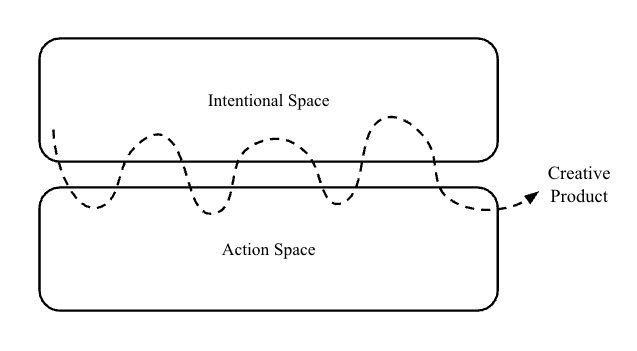
\includegraphics[width=1\linewidth]{alignedintention.png}
    \caption{A successful creative process allows users to move from intentional spaces to action spaces gracefully towards a final output. Dialogic design aims to enable this by aligning intentional spaces and action spaces.}
    \label{fig:aligned-intention}
\end{figure}

Many authors have proposed dialogue as a way to frame human-computer interaction. However, so far, there has not been any formalisation of what dialogue entails and how it can be implemented in the context of HCI, particularly in the context of human-AI co-creativity. Doing this is one of the main contributions of my thesis. 

 Proposing that humans engage in dialogue with machines is common in HCI \cite{Suchman2006-bs}. Hornbaek and Oulasvirta \cite{Hornbaek2017-wg} note that interaction is often seen as a dialogue, a cycle of perception and action. This view stresses the need for mutual understanding, making Norman’s concepts of \textbf{mapping} and \textbf{feedback} crucial. Breakdowns in this cycle are what Norman termed the \textit{gulf-of-execution} (expressing intent) and \textit{gulf-of-evaluation} (interpreting feedback).

Similarly, Allen's defining paper on Mixed-Initiative Interaction explicitly stated it was based on the properties of human dialogue, independent of modality \cite{Allen1999-sr}. He argued that mechanisms like contextual interpretation, turn-taking, and grounding are needed with any communication modality. While Yannakakis \cite{Yannakakis2014-zs} and Muller et al. \cite{Muller2020-nv} developed frameworks for mixed-initiative co-creativity, no further work developed the concept of dialogic interaction. So, in Chapter 3, I aimed to formalise dialogic interaction as a design concept, drawing from dialogue literature and HCI to construct a conceptualisation containing the following key elements:
\begin{itemize}
    \item Iteration
    \item Bidirectional communication
    \item Mutual understanding
    \item Mutual influence
    \item Shared space for creation
    \item Context awareness
\end{itemize}

In the next section, I will specifically discuss the value and limitations of each of these characteristics of dialogic design, directly addressing research question 2: "What is the potential of modelling dialogue in interaction design to enable effective human--AI co-creativity?"

In the section after that, I will derive a set of design principles from this discussion. 

\subsection{Iteration}
Iteration in creative activities involves \textbf{guided exploration} and \textbf{refinement}. This is notably hard with generative AI. As discussed in the AFR case study (Chapter 6), iteration was a main challenge. We struggled to take an image we liked and pursue that stylistic direction due to the systems' generative variability. Indeed, Park et al. \cite{Park2024-gw} found a key limitation for professional designers is "the lack of support for the iterative nature of design processes in GenAI tools".

This process is also crucial for building mental models. Iteration is needed to help users map inputs to outputs and close the gap between intention and action. While new models are beginning to afford iterative editing, interaction design can support iteration even without such capabilities. For example, in the AFR case study, I logged experiments to understand how inputs mapped to outputs.

\begin{figure}
    \centering
    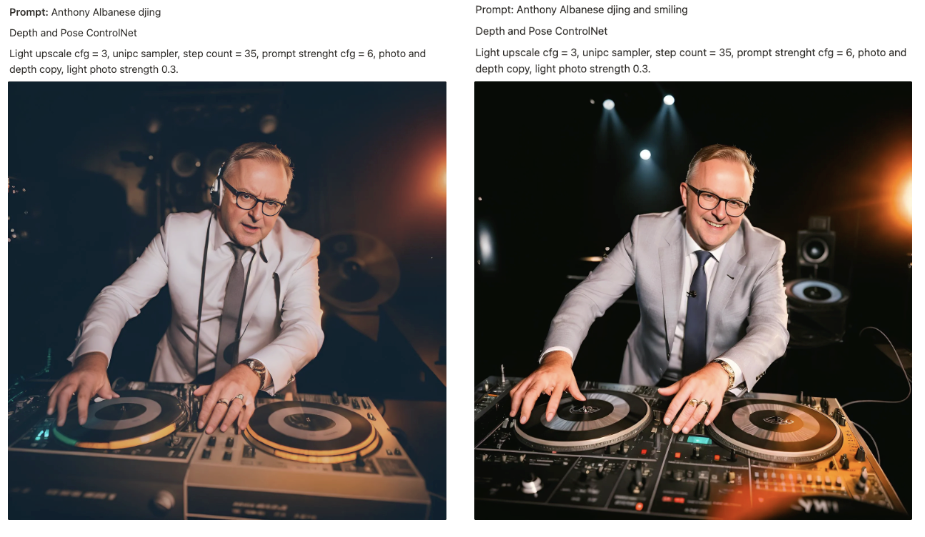
\includegraphics[width=1\linewidth]{alboexperiments.png}
    \caption{Screen-grab from my experiments log from the AFR case study, fixing some parameters while varying others. This example illustrates the difficulty of iterating with generative models. The intention was to change the facial expression of the subject, adding a single word to the prompt while using ControlNets to condition the generation. However, clothing was added, and the brightness and contrast of the image changed as well.}
    \label{fig:albo_series}
\end{figure}

This represents a clear opportunity for interaction design. Tools could have tree-like interfaces for exploration, rich histories, or afford remixing of outputs, which Zhou et al. \cite{Zhou2024-vp} found supported convergence. Another alternative is exploratory interfaces for semantic navigation. Schaerf \cite{Schaerf2024-gf} argues latent spaces are multidimensional spaces of potentiality, inviting rich exploration, a more direct implementation of the metaphor of creativity as exploration of conceptual spaces \cite{Boden2003-hk, Wiggins2019-yj}. For example, Davis et al. \cite{Davis2024-ml} showed an interface for exploring a visual space better afforded ideation than text-to-image.

\begin{figure}[H]
    \centering
    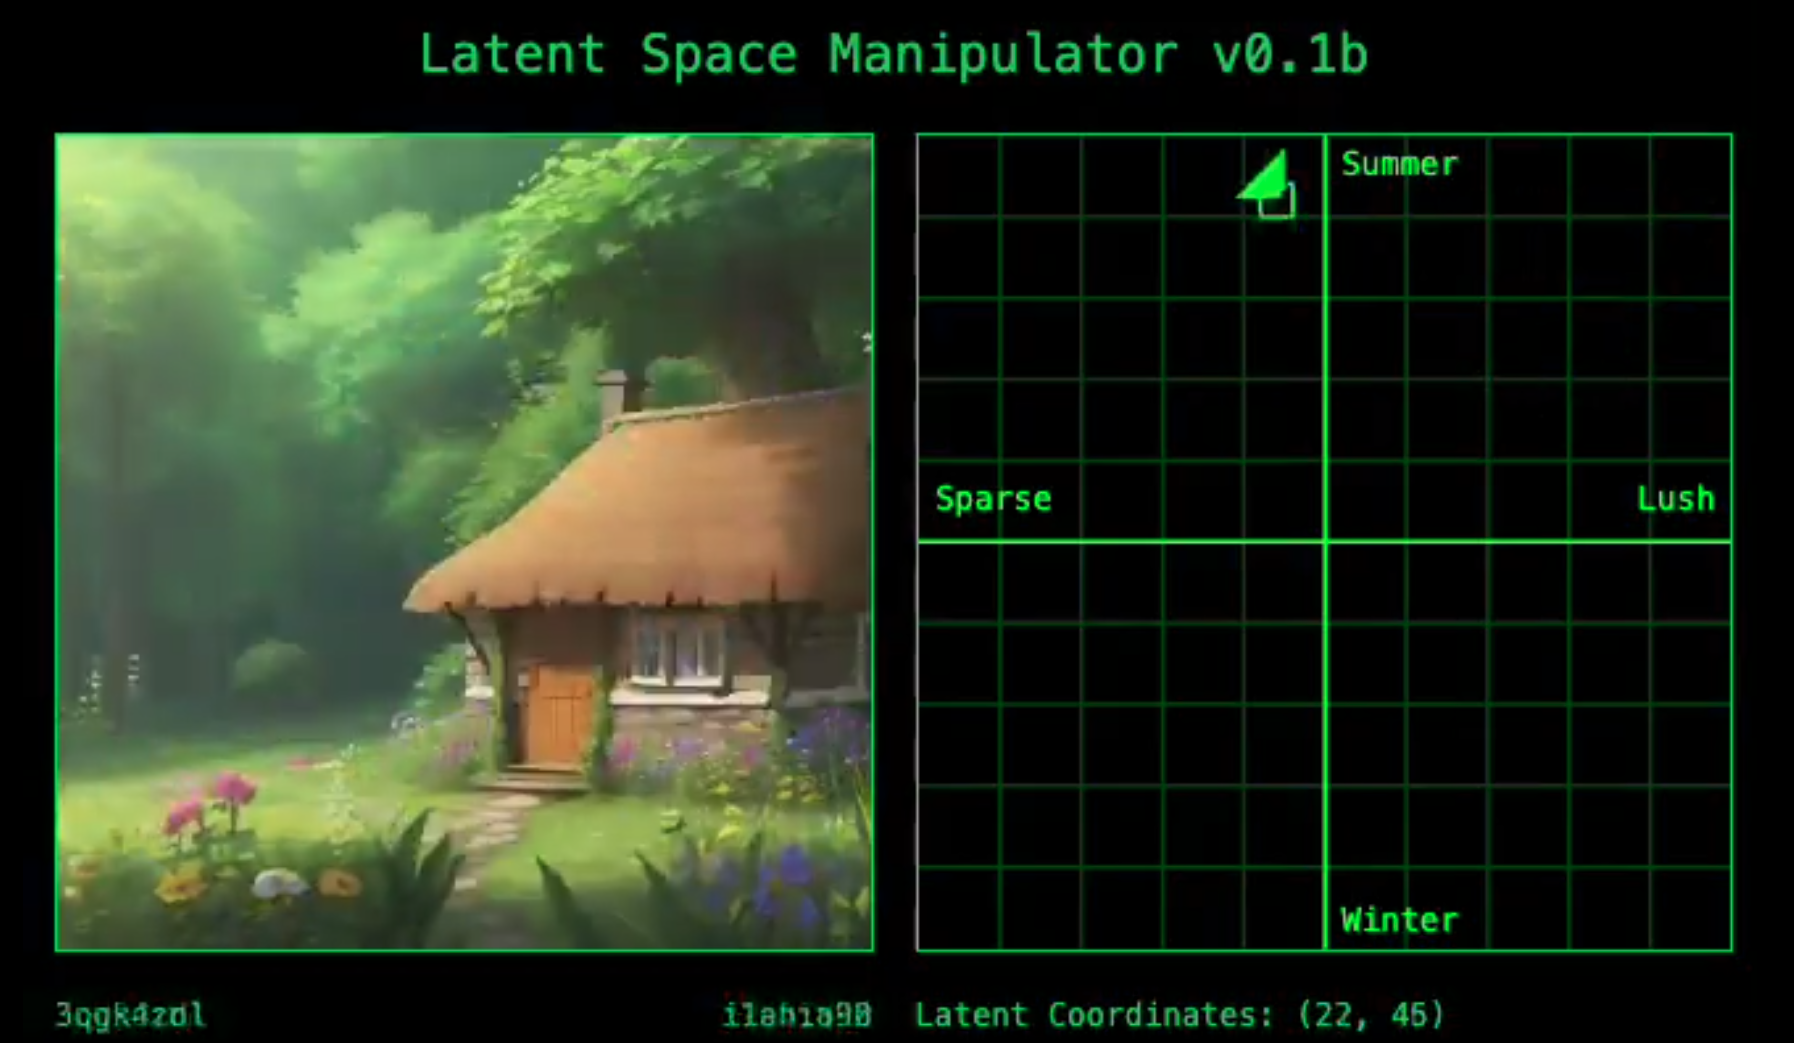
\includegraphics[width=0.8\linewidth]{latentspacemanip.png}
    \caption{Prototype by Michael Feldstein for latent space manipulation, allowing for more intuitive exploration.}
    \label{fig:feldstein}
\end{figure}

\begin{figure}[H]
    \centering
    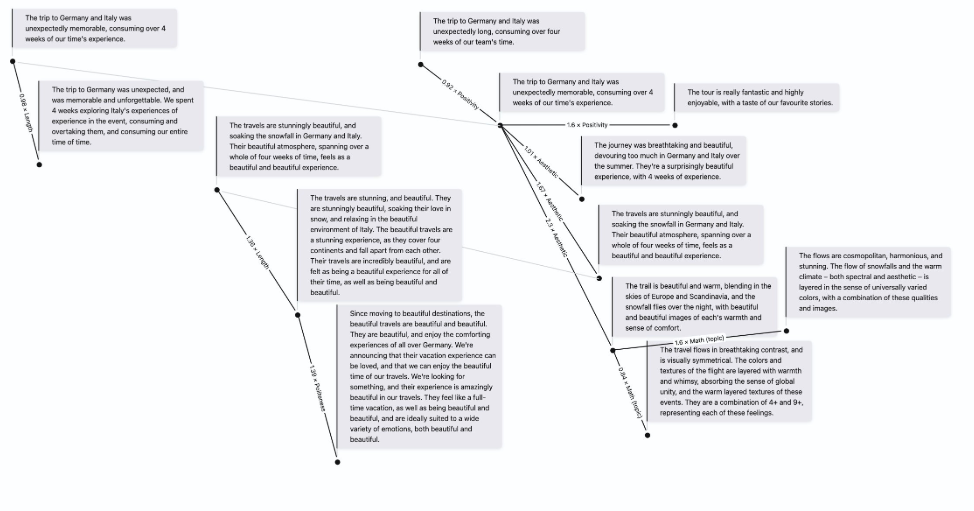
\includegraphics[width=0.8\linewidth]{linus.png}
    \caption{Linus Lee's experimental interface for exploring creative possibilities.}
    \label{fig:linus}
\end{figure}


\subsection{Bidirectional Communication and Shared Spaces}
Today, conversational interfaces are the main form of interaction with LLMs, but that was not the case at the beginning of this thesis. Interaction with LLMs and indeed most generative systems happened through instruction-response, one-shot modalities, or autocomplete functionalities. So the question of how well these systems could engage in bidirectional communication and how this could improve co-creativity was largely an open one.  My early experiments in Chapter 3 investigated this. This involved repurposing an autocomplete-based LLM into a co-authors that could engage in conversational dialogue. A key interest was to investigate whether models could switch between discussing creative goals and performing creative tasks in one single thread. These explorations showed a nascent capacity for this.
\begin{figure}[H]
    \centering
    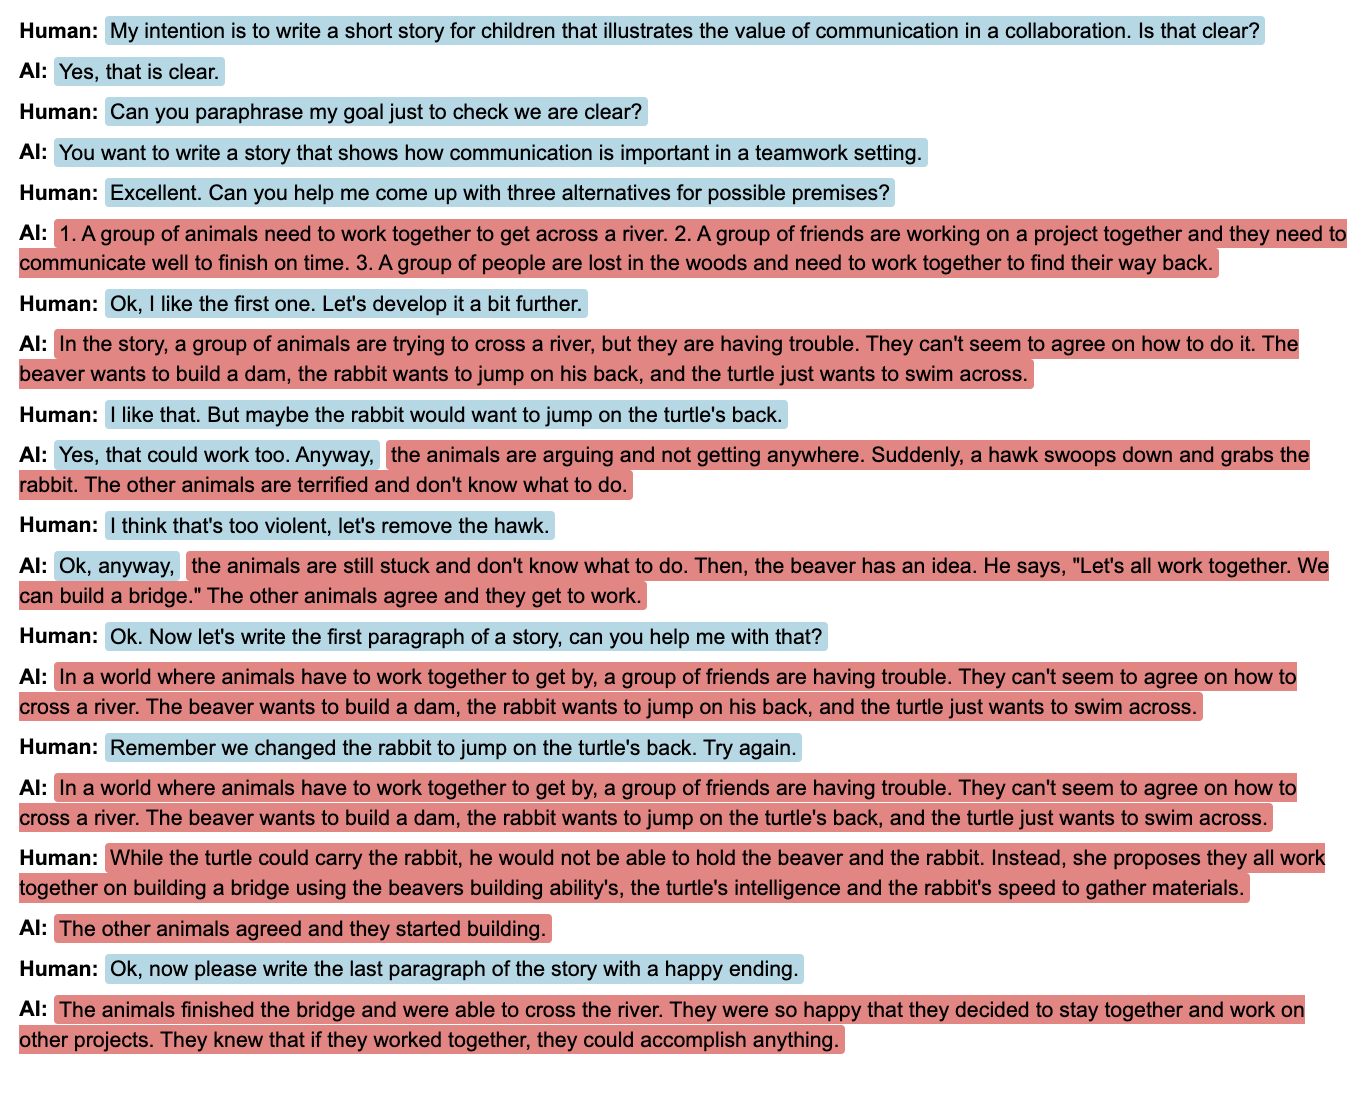
\includegraphics[width=1\linewidth]{transcriptgenchi.png}
    \caption{Transcript of an interaction with GPT-3 before the launch of ChatGPT, showing early potential for dialogic exchange.}
    \label{fig:genchi_transcript}
\end{figure}

A few months later, ChatGPT was launched, confirming the potential of bidirectional communication in terms of co-creative usefulness, as reflected in its wide adoption across creative activities. However, this also showed its limitations. As one participant noted, when interacting with a chat-based co-creator in my Chapter 4:
\begin{quote}
"At the beginning, when I was brainstorming ideas, I told Vorges ’Hi Vorges, I want to write about cyborgs.’ Vorges immediately replied with a paragraph narrating a story. I would have enjoyed a conversation first, at least to align meaning between us and feel more like we are actually collaborating." (Participant 11, Chat-only)
\end{quote}
This is an issue of conversational design, where AIs are framed as helpful assistants trained to be "helpful and harmless" \cite{Bai2022-ec, Ouyang2022-af} rather than as co-creators. It is also an issue of the interface itself, which constrains users to the intentional space through single chat-based conversational thread. A participant highlighted the limitations of ChatGPT, comparing it with an AI co-writer integrated within a text editor:
\begin{quote}
P5 said: “It can just be a bit clunky having a separate document to then copy, paste, and edit in [in ChatGPT]. This made it super seamless being in the one program.”
\end{quote}

While another participant claimed:

\begin{quote}
“ChatGPT will always rewrite the entire passage to change just one paragraph, and it’s harder to work on one text because I often need to scroll back up or continually copy and paste it.
\end{quote}

The simple idea of adding a shared editor next to a chat window to address this was the core of my Chapter 4, and it proved effective in increasing user involvement.
\begin{figure}[H]
    \centering
    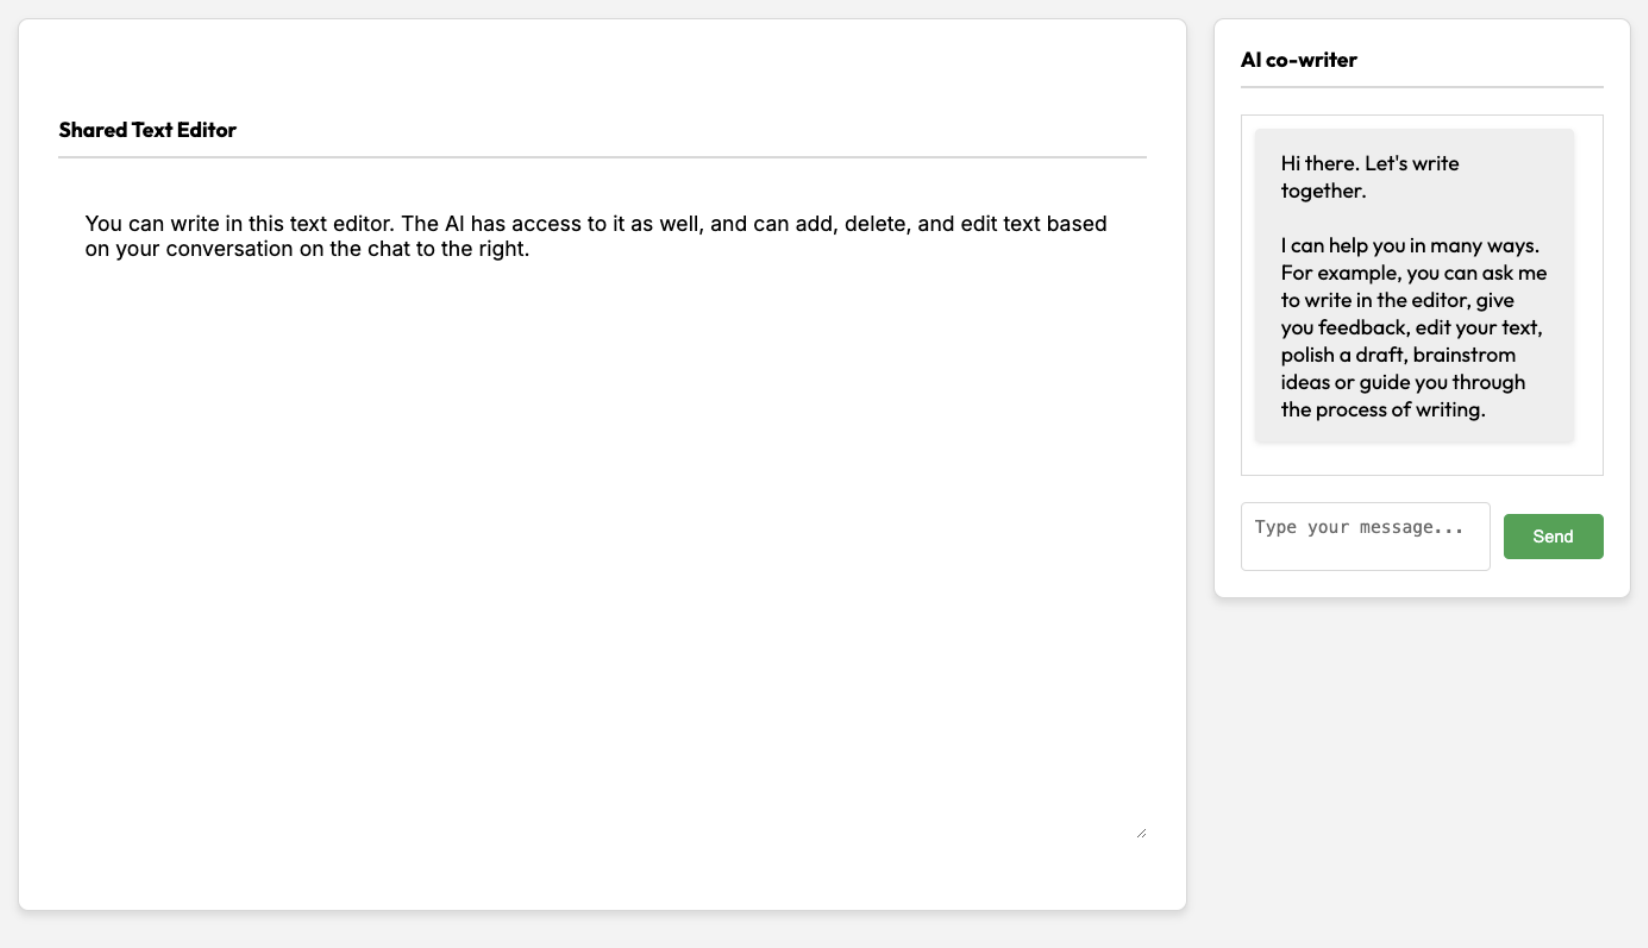
\includegraphics[width=1\linewidth]{sharededitor.png}
    \caption{The shared editor prototype, combining a chat with a direct manipulation space.}
    \label{fig:shared-editor}
\end{figure}

Participants reported more agency: P18 said, “It was much better than ChatGPT. I enjoyed how it gave me a lot more agency.” P12 remarked, “I really enjoyed it; it still let me have autonomy.” 

However, a shared space introduces challenges like managing contributions. Participants expressed this need for better visibility of introduced changes:
\begin{quote}
Participant 11: “When you ask the AI to check your grammar (as I did), it would be good if it told me what suggestions it had made, so I can double check its work easier.”

Another participant commented: “I am unsure as what parts of the text are being edited, in the end I am not quite sure which parts were mine and which ones were edited by AI.”

“Once the tool has made revisions to the original text, maybe it can highlight the key changes that have been made... otherwise I need to slowly read through and identify the changes myself.”
\end{quote}

This highlights what Buschek et al. \cite{Buschek2021-ks} call "conflicts of territory." The feedback also aligns with Amershi's Guidelines for Human-AI Interaction \cite{Amershi2019-wu} and the principle of visibility \cite{Nielsen1994-df}.

An example of a tool successfully integrating chat and a shared space is Cursor.\footnote{Cursor: \href{https://www.cursor.com/}{https://www.cursor.com/}.}

 It integrates into a known coding environment, lets the user and AI modify code, allows for chat-based interaction, tracks differences, and has version control. Its value lies not necessarily in the model (it uses out-of-the-box models such as Claude, Gemini and GPT models, which the user can select from), but in its interaction design, which created an programming co-creator integrated into user workflows. This brings us to context-awareness.
\begin{figure}[H]
    \centering
    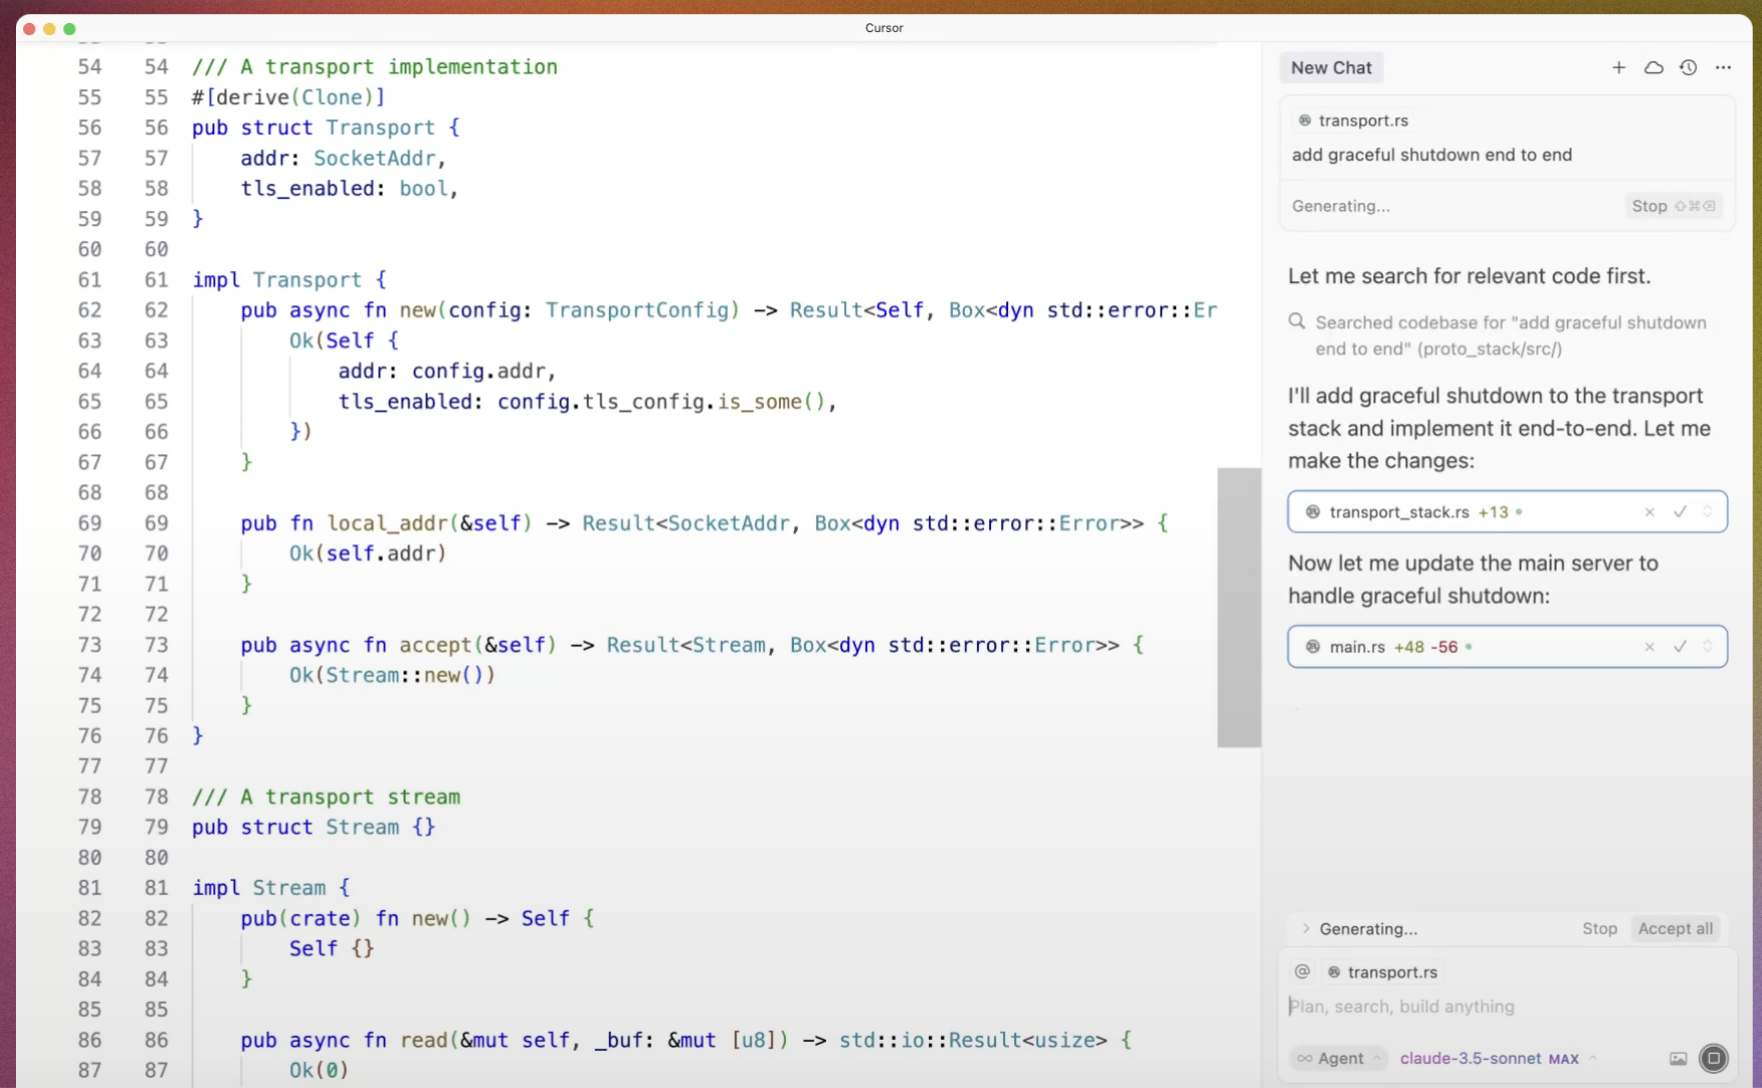
\includegraphics[width=1\linewidth]{cursor.png}
    \caption{The Cursor interface, a successful integration of a chat-based agent, shared editor, and deep contextual awareness.}
    \label{fig:cursor}
\end{figure}

\subsection{Context Awareness}
What is the value of context-awareness? This may appear as a characteristic of dialogue that is less closely related to our common understanding of dialogue between people. But upon closer examination, it becomes clear that how utterances are interpreted is highly context dependent \cite{Suchman1987-ab}.

As I discussed in Chapter 3, context can be interpreted at different levels. The first is the \textit{immediate context}, such as the live state of the creative artefact and the user's recent actions. The second, wider level encompasses the broader project context, including other files and previous work, which is relevant for making new contributions that are coherent and consistent. As in the example of Cursor above, when the user asks the model to "add a graceful shutdown at the end," the AI needs to be able to access the existing code to fulfil this request. It should do so seamlessly, without the user having to provide this context in each message. It is easy to see how this extends to other domains. In design, for example, an integrated AI co-creator would benefit from accessing a designer's existing works to align with their established style and brand guidelines.

On a third, even wider level, context can be understood as the socio-cultural, economic, and environmental context in which the co-creation happens. In design, for instance, this could help an AI co-creator produce works that align with current trends or cultural moments. It is at this third level that my installations from Chapter 7 operated. These installations were largely experimental, with the core idea being to explore how I could directly connect a generative AI—in this case, an LLM—to external data sources pertaining to local weather, CO2 levels, national economic indicators, and social media activity. The intention was to explore a \textit{situated co-creator} that could react to this environment and transform it into a piece of art or a functional soundscape by controlling a generative music engine.

While I detailed the many challenges associated with this in Chapter 7—among them, the difficulty in steering the model and its tendency to fixate on certain outputs—these installations explored a new creative possibility in sonification and new media. A new potential is afforded when an LLM is contextually situated and becomes part of a pipeline leading from the environment (social, cultural, economic or ecological) to an artwork.

Increasingly, such pipelines are becoming relevant in creative work and beyond. We see the rise of generative systems framed as agents that can be connected to data sources and tools—their context—to take actions on the user's behalf. In fact, in their systematic analysis of human and AI roles, Palani et al. \cite{Palani2024-on} identified one of the main emerging roles for the human as that of an \textit{orchestrator of workflows}. Indeed, this is an emerging practice; and it is common for creatives working with generative AI to share their custom pipelines (or keep them as a 'secret sauce') \cite{Vox2023-ab}. It seems that human and AI co-creators are beginning to operate with elements of these workflows as their creative primitives.

Tools are beginning to leverage this trend and have found significant user interest. Popular tools like \href{https://github.com/comfyanonymous/ComfyUI}{ComfyUI}, \href{https://n8n.io/}{n8n}, \href{https://flora.app/}{Flora}, and \href{https://leonardo.ai/}{Leonardo AI}'s Blueprints allow users to connect generative AI models as nodes within more complex generative and non-generative pipelines. I expect this to be a major defining thread in our future interaction with generative AI, opening many new questions, challenges, and possibilities for human-AI co-creativity.



\section{Dialogic Design Principles for Co-Creative AI Systems}

With this, I synthesise the discussions above into a set of design principles. These principles are organised along four key dimensions that are derived from the core components of dialogue previously explored: iteration, bidirectional communication, shared spaces, and context-awareness. For broader applicability, these components have been conceptualised as dimensions of \textbf{Iteration}, \textbf{Communication}, \textbf{Collaboration}, and \textbf{Integration}. Mutual influence and understanding are considered the emergent outcomes of these principles, rather than dimensions themselves.

\subsubsection{Iteration}

\textbf{Principle 1: Enable Guided Exploration.} Support the divergent phase of creativity by allowing users to explore the AI's space of possibilities. This can be achieved through interfaces that afford non-linear exploration, such as tree-like structures to pursue multiple creative paths, the ability to backtrack to previous states, navigable visual interfaces to explore the latent space, or simply ensuring the system retains recall of previous alternatives, as per Amershi \cite{Amershi2019-wu}. Such features empower users to move beyond single prompts into a more deliberate process of discovery.

\textbf{Principle 2: Facilitate Iterative Refinement.} To support creative convergence, systems can allow users to refine details of a generated output while holding other aspects constant. A common complaint by users is that the system regenerates the entire output, or introduces destructive edits when further requests or edits are provided. This is partly a technical challenge at the model level, but interaction design, however, can partly address this. For example, a text generation interface can allow a user to easily "lock" specific sentences while regenerating others. In the image domain, users can select regions to preserve, using techniques like in-painting to modify only the masked areas. Moreover, interaction design can inform training at the model level: rather than prioritising one-shot generations, systems can be trained to model iterative, multi-round editing generation processes. 

\textbf{Principle 3: Provide Editable Outputs.} Users often edit AI-generated outputs or incorporate them into separate workflows using external software. To support this process, generative systems can be designed to provide editable "building blocks" instead of monolithic, final products. For example, an image generated with distinct layers, or a piece of music provided as source-separated stems, allows users to manipulate individual components. Again, this is partly related to underlying model capabilities, and may seem unrelated to interaction design. However, I argue the role of the interaction designer is partly to inform model training to prioritise these capabilities, and to select underlying models that do have these capabilities, when available. 

\subsubsection{Communication}

\textbf{Principle 4: Clarify before generating.} Help the user navigate the variability of generative models by clarifying their prompts and instructions. For example, for a prompt like "Generate an image of a person running," the system could ask for specifics: running at night or during the day; for sport or fleeing from something; in the city or on a trail. Alternatively, the system can provide a few low-resolution options for the user to select from, before generating the final, more costly and time-consuming artefact. This clarification can be achieved without a full conversational interface, merely by presenting options.

\textbf{Principle 5: Provide a conversational space (that is not just a sycophantic echo chamber).}

Research shows that bidirectional communication increases the perception of collaboration, and the success of chat-based interfaces like ChatGPT demonstrates their practical value. However, in a co-creative context, this space should serve a purpose beyond simply executing user instructions or reinforcing their views. Indeed, recent research has shown chatbots tend to be sycophantic, biased toward praising users and reinforcing their opinions \cite{Sharma2023-or, OpenAI2025-wr}.

Through conversational design, interactions can be created to provide less agreeable feedback, ask for clarification on ambiguous requests, challenge a user's perspective, or suggest alternatives that lead to a more creative direction. As others have argued, these can be partly left to user control \cite{Moruzzi2024-cq}. Indeed, GUI affordances like sliders could allow users to control different aspects of their interaction: how creative, harsh, or opinionated they want the conversational agent to be. Ultimately, this dialogic stance helps promote the type of mutual influence and dynamic adaptation that is characteristic of successful co-creative processes, compared to a mere client-producer dynamic.

\textbf{Principle 6: Support Rich Multimodal Communication.} Enable users to communicate through rich, multimodal inputs, allowing them to "show" as well as "tell." Providing modalities to input things like images, sound snippets, sketches, gestures or data helps bridge the gap when users lack the specific vocabulary to describe their vision, offering a more direct and effective channel to articulate tacit knowledge. Moreover, this can enable new creative possibilities by enabling novel translations between modalities. 

\textbf{Principle 7: Ensure Visibility of System Capabilities.} Human-AI interaction is most effective when users clearly understand its capabilities and limitations. This can involve leveraging graphical user interfaces (GUI) and prepackaged actions to implicitly communicate this, and leverage bidirectional communication and messages to do so explicitly. This makes the system's functions discoverable and helps users form an accurate mental model of what the AI can do and how well it can do it.

\subsubsection{Collaboration}

\textbf{Principle 8: Provide a Shared Collaborative Space, Separate from the Conversational Space.} Beyond a conversational interface, where users are often limited to the \textbf{intentional space}, a \textbf{shared collaborative space}—like a canvas, editor, or timeline—can help users re-enter the \textbf{action space}. This setup allows for interaction both \textit{through} and \textit{about} the artifact, leading to a richer mutual understanding. Empowering users to participate directly in the action space helps to build their skills, prevent skill erosion, encourage active involvement, and promote the intrinsic enjoyment of \textbf{making} in the creative process. 

\textbf{Principle 9: Mediate Contributions to Manage Creative Territories.} In a shared space, the system must gracefully manage contributions to prevent "territorial conflicts," such as the AI destructively overwriting a user's manual edits. This requires clear protocols for suggestions, such as using highlights, tracked changes, or side-by-side diffs that the user can easily review, accept, or reject. Effective mediation ensures the AI's input is non-destructive, preserving user agency and sense of ownership. Moreover, this can contribute to addressing challenges of attribution, copyright and authenticity, which are becoming increasingly pressing concerns. For example, a digital artist who used AI as part of their process was recently denied copyright since they could not prove which parts were "made by him" and which ones "by the AI" \cite{US-Copyright-Office-Review-Board2023-nw}. However, it is worth noting that this may contradict the very definition of co-creativity, which posits a blending of creativities where outputs are hard to attribute to one or the other \cite{Davis2013-jy}. 

\subsubsection{Integration}

\textbf{Principle 10: Embed the AI within the User's Workspace.} Maximise usefulness by integrating directly into the user's existing workspace and work context. For instance, for music, this means integrating with DAWs like Ableton; for design, directly into professional design software; for writing, into text editing software; and for code, into a preferred IDE (like Cursor, a VSCode fork). Additionally, this integration may also involve accessing relevant files and work with user consent --such as existing codebases, design assets, brand guidelines, and previous written works. This can contribute to AI contributions that are more readily integrated and aligned with the user's work. 

\textbf{Principle 11: Enable Awareness of Wider Sociocultural Context.} Enhance the AI's relevance by allowing it to reference the wider, socially situated context in which creation occurs. This could involve bringing in external information like current trends, data feeds, or cultural events. In the case of my new media installations, this involved piping information from external data feeds that changed in real-time. One can imagine a design co-creators integrated with constantly updating Pinterest feeds, social media, and any feed that could make contributions more socially and culturally relevant. 

\textbf{Principle 12: Facilitate Human Orchestration of Flexible Workflows.} Design the co-creative system as a modular component that can be part of a larger, human-directed pipeline. By enabling interoperability, the system allows the user to act as an "orchestrator," connecting the AI to other data sources, generative models, or software tools. This empowers users to build bespoke creative workflows, positioning the AI as a powerful and flexible component within their individual process.

\section{Contribution and Future Directions}
This thesis argued that the current paradigm of human-AI interaction often leads to \textit{severed agency}. The primary contribution is the development of \textit{dialogic design} as a framework to counteract this by more closely aligning intention and action through the principles organised under the dimensions of \textbf{Iteration}, \textbf{Communication}, \textbf{Collaboration}, and \textbf{Integration}. The design principles derived from this research offer concrete guidance for building effective co-creative tools that maintain human agency and allow people to leverage the potential of generative AI.

   
    \clearpage
   
    %appendices
    \appendix
    \chapter[Appendix: a]{Supplementary Materials}\label{a:supps}


    \chapter{Documentation}\label{a:documentation}


   
    \clearpage
    
    \backmatter
    
    \pagestyle{noHeading}
    \bibliographystyle{apalike}
    \bibliography{paperpilewhole}

\end{document}
